% Opsætter KU Tex dokument
%%%%%%%%%%%%%%%%%%%%%%%%%%%%%%%%%%%%%%%%%%%%%%%%%%%%%%%%%%%%%%%%%%%%%%%%%%%%%%%%
\documentclass{article}                                                        %
\usepackage[a4paper, hmargin={2.8cm, 2.8cm}, vmargin={2.5cm, 2.5cm}]{geometry} %
\usepackage{eso-pic}  % \AddToShipoutPicture                                   %
\usepackage{graphicx} % \includegraphics                                       %
%\usepackage{subfig} - Can not be used with subcaption package (for subfigures)
\usepackage{setspace}                                                        %
%%%%%%%%%%%%%%%%%%%%%%%%%%%%%%%%%%%%%%%%%%%%%%%%%%%%%%%%%%%%%%%%%%%%%%%%%%%%%%%%

% Pakker til skrifttyper, tekst osv.
%%%%%%%%%%%%%%%%%%%%%%%%%%%%%%%%%%%%%%%%%%%%%%%%%%%%%%%%%%%%%%%%%%%%%%%%%%%%%%%%
    \usepackage[utf8]{inputenc}  % Implementere Unicode                        %
    \usepackage[T1]{fontenc}     % Unicode skrifttype fx. é skrives som 1 tegn %
    \usepackage[english]{babel}   % Dansk Ordbog                                %
    \usepackage{microtype}       % Forbedre linjeombrydningen                  %
    \usepackage{libertine}       % Skrifttype                                  %
%%%%%%%%%%%%%%%%%%%%%%%%%%%%%%%%%%%%%%%%%%%%%%%%%%%%%%%%%%%%%%%%%%%%%%%%%%%%%%%%

% Pakker til matematik og kode.
%%%%%%%%%%%%%%%%%%%%%%%%%%%%%%%%%%%%%%%%%%%%%%%%%%%%%%%%%%%%%%%%%%%%%%%%%%%%%%%%
    \usepackage{mathtools}       % Udvidelse til amsmath pakken                %
    \usepackage{amsthm}          % Pakke til bevisførelse                      %
    \usepackage{amssymb}         % Extra matematiske symboler                  %				
	\usepackage{mychemistry}												   %
	\usepackage[version=3]{mhchem}											   %
	\usepackage{wrapfig}													   %
	\usepackage{siunitx}	
	\usepackage{anyfontsize}
	\usepackage{ragged2e}
	\usepackage{algorithm2e}
	\usepackage[final]{pdfpages}
	\usepackage{listings}
	\usepackage{tikz}
	\usepackage{multirow}
	\usepackage{makecell}
	\usepackage{fourier} 
	\usepackage{array}
	\usepackage{todonotes}
	\usepackage{pdflscape}
	\usetikzlibrary{arrows,shapes}
	\usepackage{titlesec}
	\usepackage{hyperref}
	\usepackage{url}
	\usepackage[nottoc,numbib]{tocbibind}
	\usepackage{semantic}
	\usepackage{subcaption}
	\usepackage{qtree}
	\usepackage{hhline}
	
	\definecolor{light-gray}{gray}{0.85}
	\lstset{
	    	numbers=left,
	    	breaklines=true,
	    	backgroundcolor=\color{light-gray},
	    	tabsize=2,
	    	basicstyle=\ttfamily,
	    	literate={\ \ }{{\ }}1
	}
	
	\urlstyle{same}
	\tikzstyle{vertex}=[circle,fill=white!25,minimum size=20pt,inner sep=0pt]
	\tikzstyle{edge} = [draw,thick,-]

	\definecolor{light-gray}{gray}{0.85}
	\definecolor{dkgreen}{RGB}{0.0,128.0,43.0}
	\lstdefinelanguage{FSharp}%
{morekeywords={new, match, with, rec, open, module, namespace, type, of, member, % 
and, for, while, true, false, in, do, begin, fun, function, return, yield, try, %end
mutable, if, then, else, cloud, async, static, use, abstract, interface, inherit, finally, int },
  otherkeywords={ let!, return!, do!, yield!, use!, var, from, select, where, order, by },
  keywordstyle=\color{bluekeywords},
  sensitive=true,
  basicstyle=\ttfamily,
	breaklines=true,
  xleftmargin=\parindent,
  aboveskip=\bigskipamount,
	tabsize=4,
  morecomment=[l][\color{dkgreen}]{///},
  morecomment=[l][\color{dkgreen}]{//},
  morecomment=[l][\color{dkgreen}]{(*},
  morecomment=[s][\color{dkgreen}]{},
  morestring=[b]",
  showstringspaces=false,
  literate={`}{\`}1,
  stringstyle=\color{redstrings},
}
	
	
												   %
%%%%%%%%%%%%%%%%%%%%%%%%%%%%%%%%%%%%%%%%%%%%%%%%%%%%%%%%%%%%%%%%%%%%%%%%%%%%%%%%

% Pakker til layout.
%%%%%%%%%%%%%%%%%%%%%%%%%%%%%%%%%%%%%%%%%%%%%%%%%%%%%%%%%%%%%%%%%%%%%%%%%%%%%%%%
    \usepackage{fancyhdr}            % Gør det muligt at bruge sidehoveder     %
    \usepackage{graphicx}            % Mulighed for bl.a. \includegraphics     %
    \usepackage{colortbl}            % Hvis man vil farvelægge sine tabeller   %
    \usepackage{array}               % Gør miljøerne array og tabular bedre    %
    \usepackage{parskip}             % Første paragraf i afsnit indrykkes ikke %
    \usepackage{titlesec}            % Tilpassing af afstand mellem sektioner  %
    \usepackage[lastpage,user]{zref} % Side x af y                             %
%%%%%%%%%%%%%%%%%%%%%%%%%%%%%%%%%%%%%%%%%%%%%%%%%%%%%%%%%%%%%%%%%%%%%%%%%%%%%%%%


% Implementerer en række makroer og de pakker der er importeret
%%%%%%%%%%%%%%%%%%%%%%%%%%%%%%%%%%%%%%%%%%%%%%%%%%%%%%%%%%%%%%%%%%%%%%%%%%%%%%%%
    \pagestyle{fancy}                        % Implementerer sidehoved         %
    \lhead{University of Copenhagen}                % Venstre sidehoved               %
    \rhead{Casper Bresdahl}                             % Højre sidehoved      %
    \cfoot{\thepage\ of \zpageref{LastPage}} % Side x af y                     %
    \newtheorem*{prp}{Propostion}            % Skaber nyt theorem  
    \renewcommand{\baselinestretch}{1.25}       %
%%%%%%%%%%%%%%%%%%%%%%%%%%%%%%%%%%%%%%%%%%%%%%%%%%%%%%%%%%%%%%%%%%%%%%%%%%%%%%%%

% Mindsker afstanden mellem sektioner
%%%%%%%%%%%%%%%%%%%%%%%%%%%%%%%%%%%%%%%%%%%%%%%%%%%%%%%%%%%%%%%%%%%%%%%%%%%%%%%%%%
\titlespacing\section{0pt}{12pt plus 4pt minus 2pt}{0pt plus 1pt minus 3pt}      %
\titlespacing\subsection{0pt}{12pt plus 4pt minus 2pt}{0pt plus 1pt minus 3pt}   %
\titlespacing\subsubsection{0pt}{12pt plus 4pt minus 2pt}{0pt plus 1pt minus 3pt}%
%%%%%%%%%%%%%%%%%%%%%%%%%%%%%%%%%%%%%%%%%%%%%%%%%%%%%%%%%%%%%%%%%%%%%%%%%%%%%%%%%%

%Ændrer størelsen på sections
%%%%%%%%%%%%%%%%%%%%%%%%%%%%%%%%%%%%%%%%%%%%%%%%%%%%%%%%%%%%%%%%%%%%%%%%%%%%%%%%%%
\titleformat{\section}
{\normalfont\fontsize{14}{16}\bfseries}{\thesection}{1em}{}
\titleformat{\subsection}
{\normalfont\fontsize{12}{14}\bfseries}{\thesubsection}{1em}{}
\titleformat{\subsubsection}
{\normalfont\fontsize{11}{13}\bfseries}{\thesubsubsection}{1em}{}
%%%%%%%%%%%%%%%%%%%%%%%%%%%%%%%%%%%%%%%%%%%%%%%%%%%%%%%%%%%%%%%%%%%%%%%%%%%%%%%%%%

%%%%%%%%%%%%
% Document %
%%%%%%%%%%%%

\begin{document}

\begin{titlepage}

\newcommand{\HRule}{\rule{\linewidth}{0.5mm}} % Defines a new command for the horizontal lines, change thickness here

\begin{center}
 % Center everything on the page
 
%----------------------------------------------------------------------------------------
%	HEADING SECTIONS
%----------------------------------------------------------------------------------------

\textsc{\LARGE University of Copenhagen}\\[1.5cm] % Name of your university/college
\textsc{\Large Computer Science}\\[0.5cm] % Major heading such as course name
\textsc{\large }\\[0.5cm] % Minor heading such as course title

%----------------------------------------------------------------------------------------
%	TITLE SECTION
%----------------------------------------------------------------------------------------

\HRule \\[0.4cm]
{ \huge \bfseries Punctae Segmentation for Measuring Transcytosis Across the Blood–brain Barrier}\\[0.4cm] % Title of your document
\HRule \\[1.5cm]
 
%----------------------------------------------------------------------------------------
%	AUTHOR SECTION
%----------------------------------------------------------------------------------------

\begin{minipage}{0.4\textwidth}
\begin{flushleft} \large
\emph{Author:}\\ 
% Your name
Casper \textsc{Bresdahl} \\
\end{flushleft}
\end{minipage}
~
\begin{minipage}{0.4\textwidth}
\begin{flushright} \large
\emph{Teacher:} \\
Martin \textsc{Lillholm}
\end{flushright}
\end{minipage}\\[2cm]

% If you don't want a supervisor, uncomment the two lines below and remove the section above
%\Large \emph{Forfattere:}\\
%Axel \textsc{Christof}\\% Your name
%Casper \textsc{Bresdahl}\\
%Emilie \textsc{Bentsen}\\[1cm] 

%----------------------------------------------------------------------------------------
%	DATE SECTION
%----------------------------------------------------------------------------------------

{\large \today}\\[2cm] % Date, change the \today to a set date if you want to be precise

%----------------------------------------------------------------------------------------
%	LOGO SECTION
%----------------------------------------------------------------------------------------


\includegraphics{logo.png}\\[1cm] % Include a department/university logo - this will require the graphicx package
 
%----------------------------------------------------------------------------------------

\vfill % Fill the rest of the page with whitespace

%Disse linjer skaber forside, evt indholdsfortegnelse, og sætter sidetal
%%%%%%%%%%%%%%%%%%%%%%%%%%%%%%%%%%%%%%%%%%%%%%%%%%%%%%%%%%%%%%%%%%%%%%%%%%%%%%%%
									                                           %
    \thispagestyle{empty}   % Fjerner sidetal forside                          %
        % Slå disse til hvis der ønskes indholdsfortegnelse                    %
        %%%%%%%%%%%%%%%%%%%%%%%%%%%%%%%%%%%%%%%%%%%%%%%%%%%%%%%%%%%%%%%%%%%%%%%% 
            \newpage                % Side til indholdsfortegnelse            %
            %\thispagestyle{empty}   % Fjerner sidetal fra indholdsfortegnelse %
            %\tableofcontents        % Skaber indholdsfortegnelse              %
    \end{center}
    %\section*{Forord}
    	
		
        %%%%%%%%%%%%%%%%%%%%%%%%%%%%%%%%%%%%%%%%%%%%%%%%%%%%%%%%%%%%%%%%%%%%%%%%
    \newpage                % Første rigtige side
    \setcounter{page}{1}    % Sætter rigtigt sidetal på første side
%%%%%%%%%%%%%%%%%%%%%%%%%%%%%%%%%%%%%%%%%%%%%%%%%%%%%%%%%%%%%%%%%%%%%%%%%%%%%

\end{titlepage}
{\fontsize{10}{14}\selectfont
\section{Introduction}
In this thesis project we will look into how machine learning can be used in the treatment of colitis. Colitis is a chronic digestive disease which is characterized by inflammation of the inner lining of the colon. Suffering from colitis causes pain and discomfort to the abdomen and often causes diarrhea with or without blood\cite{colitis}. Often four different treatments are prescribed, depending on the scope of inflammation in the colon. Local 5-ASA is a mild suppository if the inflammation does not stretch too far into the colon. Oral 5-ASA is a mild treatment and is prescribed if the inflammation is mild but stretches far into the colon. Oral steroid is a moderate treatment and is prescribed if the inflammation is severe, but not necessarily stretched far into the colon. Lastly IV steroids is a harsh treatment prescribed if the inflammation is severe and is stretched far into the colon.\\
In this thesis work, several deep neural networks were trained to detect inflammation in individual frames of endoscopy examinations in an attempt to draw segmentations of these videos. As the inflammation stretches into the colon without 'holes', it was attempted to predict this separation point, where we go from an inflamed colon to a healthy colon. Such a segmentation and separation point could then be used by a doctor to determine the correct treatment. However, the segmentations were also used to train other machine learning models to predict which treatment patients should be prescribed. One could imagine these results being used as a second opinion for a doctor.

The thesis work is divided into five sections. In the first, the theory used for this project is presented. In the second section the methods used throughout the thesis work is presented and goes into details about data pre-processing, how separation point predictions were made,  how treatment predictions were made and how the predictions were refined and then used for predictions again. Next the results of the thesis work will be presented before we go into a discussion about the results and end with a conclusion.
\section{Theory}
\subsection{Two-photon microscopy}
Two-photon microscopy is a fluorescence imaging technique, where two photons are brought to an excitation state at the same time and then absorbed to emit a photon of fluorescence. As the wavelength of the two excited photons is required to be longer than the emitted light, near-infrared excitation light is often used. Because of the multi photon absorption, the background signal is strongly suppressed, and because using infrared light minimizes scattering in tissue, two-photon microscopy gets an increased penetration depth over confocal microscopy, which uses a spatial pinhole technique to block out-of-focus light \cite{confocal}. Due to this increased penetration depth, two-photon microscopy can be used to obtain images of living tissue up to one millimetre in thickness \cite{wikimicroscopy}. For this project, this means two-photon microscopy can be used to measure transcytosis through the blood-brain barrier. This is done in \cite{imaging} where the change in blood-brain barrier permeability of small molecules is measured after injection of fluorophore, a compound which emits photons upon excitation. In more detail this was done by using two-photon microscopy in vivo in mice, where the anesthetized mice's brains were imaged through a craniotomy over the somatosensory cortex. The light emitting fluorophore signal can then be measured in both the blood vessels and brain parenchyma. The used two-photon microscopy allows for imaging at different depths in the tissue and can be compiled to a three dimensional reconstruction of the brain microvasculature. \autoref{puncta} shows a cross section of such reconstructions and thus how the transcytosis in the blood-brain barrier has been affected. With time, the fluorophore coalesce into numerous puncta of vescicles. In \autoref{puncta} we see these puncta of vesicles which accumulate around the blood-brain barrier interface. The three dimensional reconstruction can be sliced in different ways to give different perspectives of the results. Imagining the reconstruction as a block \autoref{puncta} is likely images where the block has been sliced from top to bottom. One could also slice the block from left to right giving a view of the 'insides' of the arteries where we would then see the puncta coalesce in a circle around the blood-brain barrier interface. 
%\begin{figure}[H]
%	\centering
%	\begin{subfigure}[b]{\linewidth}
%		\centering
%		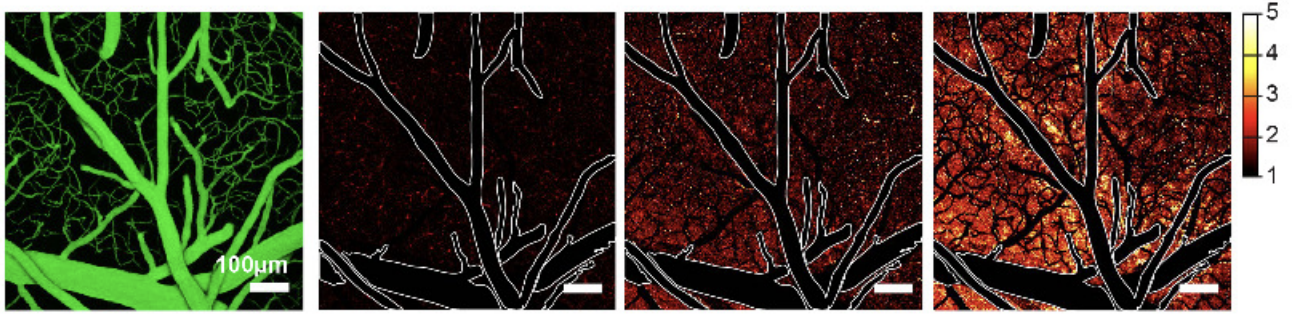
\includegraphics[width=0.9\linewidth]{Materials/Theory/paperres}
%		\caption{Cross section time lapse images with injection of NaFluo. We see an accumulation of NaFluo in the brain parenchyma over a period of 30 minutes. Image taken from \cite{imaging}.}
%		\label{paperres}
%	\end{subfigure}
%	\\
%	\begin{subfigure}[b]{\linewidth}
%		\centering
%		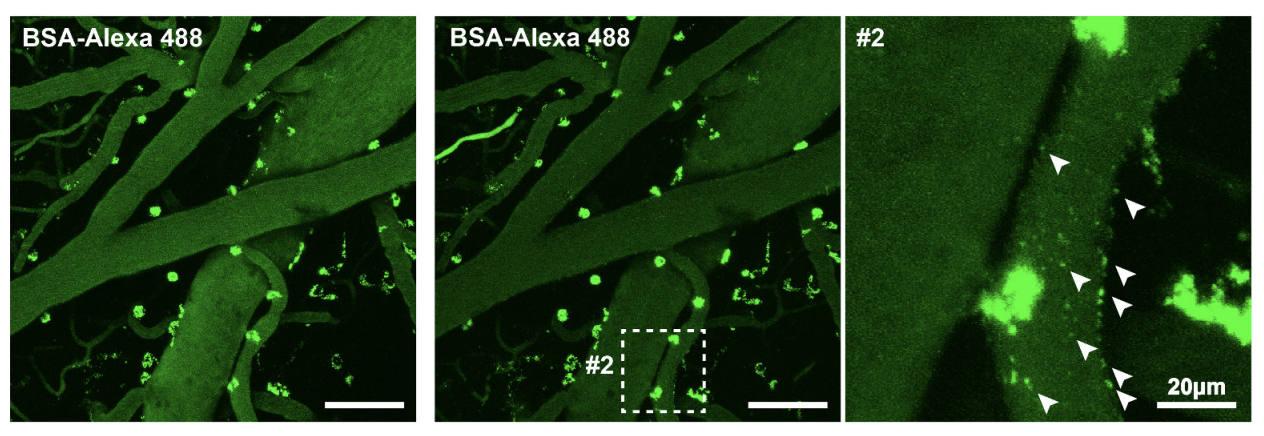
\includegraphics[width=0.7\linewidth]{Materials/Theory/puncta}
%		\caption{Coalescence of BSA-Alexa 488 after 60 and 120 minutes. White arrows indicate puncta we are interested in finding. Image taken from \cite{imaging}.}
%		\label{puncta}
%	\end{subfigure}
%\end{figure}
\begin{figure}
	\centering
	\begin{subfigure}[b]{0.2\linewidth}
		\centering
		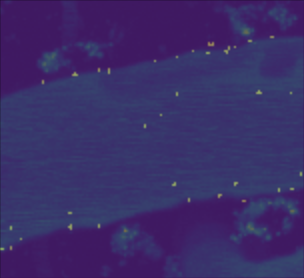
\includegraphics[width=\linewidth]{Materials/Theory/series1}
	\end{subfigure}
	\qquad
	\begin{subfigure}[b]{0.2\linewidth}
		\centering
		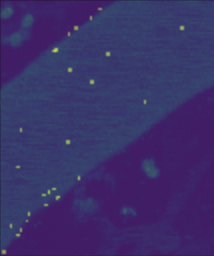
\includegraphics[width=0.77\linewidth]{Materials/Theory/series2}
	\end{subfigure}
	\qquad
	\begin{subfigure}[b]{0.2\linewidth}
		\centering
		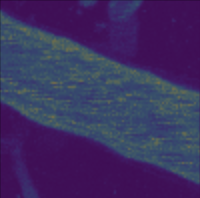
\includegraphics[width=0.94\linewidth]{Materials/Theory/series3}
	\end{subfigure}
	\caption{Cross section images of reconstruction taken from the training data and overlaid with the true masks indicating puncta we are interested in finding.}
	\label{puncta}
\end{figure}
\newpage
\subsection{Convolutional layers}
\begin{wrapfigure}{r}{0.3\linewidth}
	\vspace{-1.2cm}
	\centering
	\begin{subfigure}[b]{\linewidth}
		\centering
		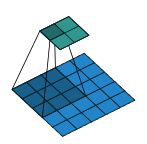
\includegraphics[width=0.6\linewidth]{Materials/Theory/convolution}
		\caption{Convolution of a 5x5 input image with a 3x3 kernel using no padding and 1 stride, producing a 2x2 output image.}
		\label{convolution}
	\end{subfigure}
	\\
	\begin{subfigure}[b]{\linewidth}
		\centering
		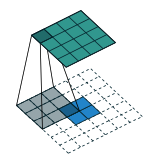
\includegraphics[width=0.6\linewidth]{Materials/Theory/transposedconv}
		\caption{Transposed convolution of a 2x2 input image with a 3x3 kernel using 2 'layers' of padding all around and 1 stride, producing a 4x4 output image.}
		\label{transposedconv}
	\end{subfigure}
	\caption{Examples of a convolution and a transposed convolution. Blue layer denotes input image, cyan layer denotes output image, shaded squares denotes kernel and dotted squares denotes padding. Images are from \cite{convolutionarticle}.}
\end{wrapfigure}
In the convolution layers a (discrete) convolution is performed. A (discrete) convolution is an operation in which a kernel is moved over a signal and the output is the sum of products between the kernel and the overlapping elements. In our concrete case we are dealing with images, which can be thought of as an array of pixel values. If we simplify the discussion to greyscale images, we simply have an array of same dimension as the image filled with pixel intensities. We can now overlay the input image with our kernel and compute the sum of products. We can now move the kernel over the image, and each time we move the kernel we get an output. The number of pixels we move the kernel is called the \textit{stride}. After having moved the kernel over the entire image, the output is a new image which dimensions are smaller than the input. How much smaller depends on the stride and the kernel size. If a certain output dimension is needed after a convolution, the input images might need to be padded with 'extra' pixels. Several strategies exists for padding, the most common is to pad with zeros. An illustration of a convolution can be seen in \autoref{convolution} \cite{convolutionarticle}.

\subsection{Max pooling layers}
In the max pooling layers a kernel is defined and moved around the input image. The output is then the largest value inside the kernel. The number of pixels it is moved is again determined by a stride. A max pooling layer using a 2x2 kernel and a stride of 2 thus halves both input image dimensions as a 2x2 area in the input image becomes a single pixel in the output image \cite{convolutionarticle}.

\subsection{Transposed convolutions}
In the upsampling layers we want to perform a 'reversed' convolution where we go from a small image to a larger image while still keeping the connectivity pattern. The 'up-conv' layer used in \autoref{unet} is also called a \textit{transposed convolution}, and we perform these instead of simply upscaling the image because we can learn an optimal way of upscaling the images. To perform a transposed convolution we compute the output shape of a convolution with a given input shape and then we invert the input and output shapes. The input would then be padded with zeroes to comply with the kernel size. As an example we would like to perform a convolution with a 3x3 kernel on a 4x4 input image with no padding and 1 stride. This would produce a 2x2 output image. Inverting the input and output, we would then have to convolve a 2x2 image with a 3x3 kernel to get a 4x4 output. As the 2x2 image does not comply with the 3x3 kernel, we pad it with 2 'layers' of zeroes all around. An illustration of a transposed convolution can be seen in \autoref{transposedconv}. Although this is not the most efficient way of performing a transposed convolution, it gives an intuition of what is happening \cite{convolutionarticle}.

\subsection{Convolutional Neural Networks}
\begin{wrapfigure}{l}{0.6\linewidth}
	\centering
	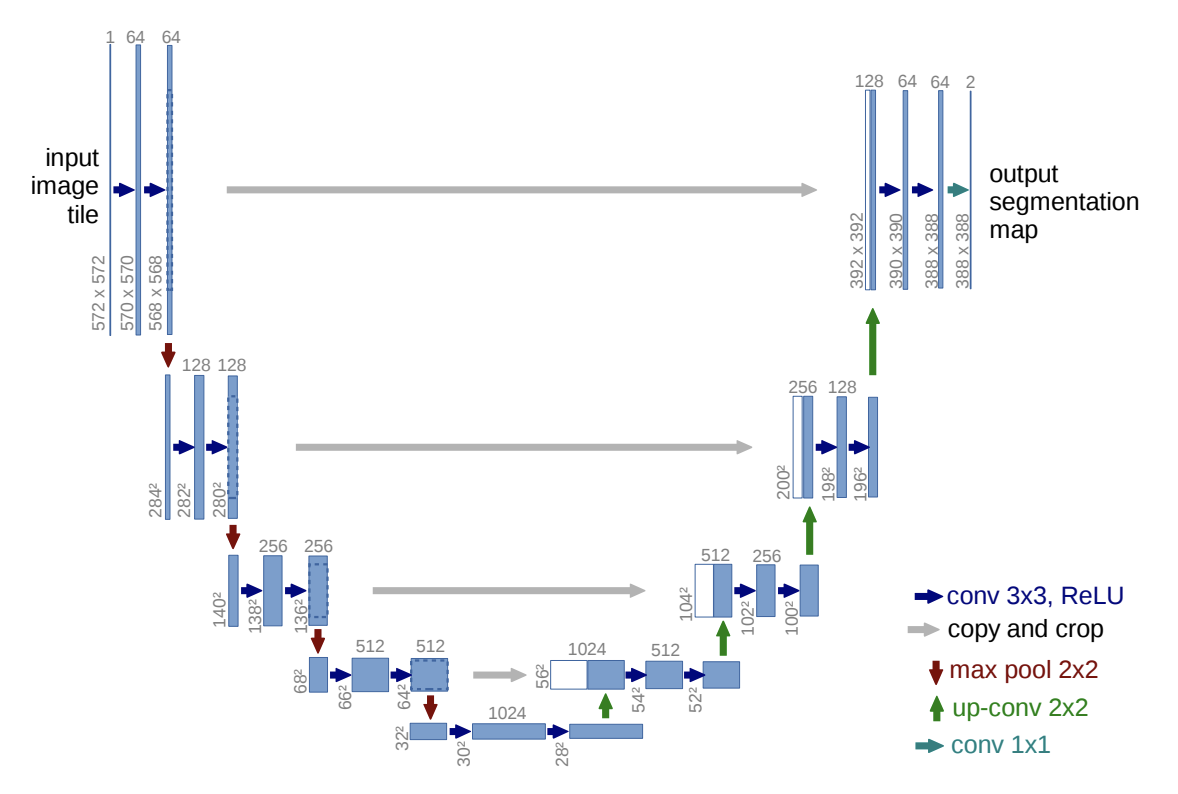
\includegraphics[width=\linewidth]{Materials/Theory/unet}
	\caption{U-Net architecture example for input image of size 572x572 pixels. Image taken from \cite{unetarticle}}
	\label{unet}
\end{wrapfigure}
Deep neural networks (DNN's) are neural networks with several layers between the input and the output which allows them to learn complex non-linear relationships in the data. Each layer holds a number of neurons which usually are fully connected, meaning each output from the neurons in the previous layer goes into the neurons of the next layer. DNN's have a lot of parameters which are getting trained as each neuron have their own weight. A convolutional neural network (CNN) is a special class of DNN's which mainly uses convolutional layers. This makes it possible to process images as it is the weights of a kernel which are trained rather than processing each individual pixel in the images. CNN's are usually used for image segmentation or in general tasks which requires processing of images. A concrete example of a CNN could be a modified U-Net model where the encoder is replaced by a ResNet-18 model. The original U-Net architecture can be seen in \autoref{unet}.\\
The U-Net architecture can be split in two parts, a left part which downscales the processed image and a right half which upscales the image again. Replacing the encoder of the U-Net model means this left part is replaced with the ResNet-18 model. ResNet-18 begins by performing a 7x7 convolution with a stride of two followed by a 3x3 max pooling with a stride of two. It then follows a pattern of doing two 3x3 convolutions each followed by a rectified linear unit operation before a skip connection, skipping two convolutions. After three convolutions the fourth uses a stride of two to downsample the image. This results in the feature map getting halved in size and the number of the feature channels getting doubled after each downsampling step. Three downsamplings are done this way before we reach the right half of the U-Net model \cite{resnet}. For the right half, an upsampling followed by a 2x2 convolution is performed. This halves the number of feature channels and doubles the size of the feature map. Then a concatenation from the corresponding left half feature map is done. These skips (along with whose in the ResNet-18 model) allows the model to recover lost spatial information and alleviates the vanishing gradient problem, which results in improved performance. After the skips, two 3x3 convolutions are performed each followed by a rectified linear unit operation. In the end a 1x1 convolution is performed to map the final feature map to the correct number of prediction classes \cite{unetarticle}. Another example of a CNN is LinkNet which in a similar fashion as to U-Net has a left part which downsamples images and a right path which then upsamples them with skip connection in between, but instead of concatenating the feature maps after these skips, in LinkNet they are added. This reduces the number of parameters the network needs to learn \cite{linknet}.\\
The clear advantages of CNN's are how accurate and how fast the models can make predictions. This allows for fast automatisation of suited tasks. However, it might take weeks to train state of the art models without any guarantees if it will perform better than its predecessor, and so it is a time consuming process to develop good models. It is also taxing on power consumption and the environment to train for these long periods of time. Often times the most limiting factor in model development is gathering varied data or annotating this data.

\subsection{Transfer learning}
Transfer learning is a common technique where a model developed for some task is reused as starting point for another model. This allows the model to get a 'head start' as it has already learnt a set of features to detect. The ImageNet project is a large database consisting of more than 14 million images in over 20 thousand categories \cite{trasnferlearning}. It is very common to use transfer learning with a model trained on the ImageNet data as this gives a broad foundation, and further training then 'specializes' the model to the specific task at hand.

\subsection{Optimization}
%When we in this project want to train a model, we want its input to be the two-photon microscopy images of mice brains and we want the outputs to be the locations of vescicles puncta. To train the model we thus need an annotated dataset, where each puncta has been marked by hand by an expert in the field. The CNN is then trained by supervised learning to predict the location of the puncta. Our data is split into a training, validation and test set such that we can compare models and tune hyper-parameters on unknown data (the validation set) and we can measure the models' unbiased performance (the test set). 
For optimization, the stochastic gradient descend (SGD) based learning algorithm \textit{Adam} is often used. SGD is an iterative method for optimization and can intuitively be thought of as having a ball rolling on a hill landscape, SGD finds the direction of steepest descend and takes a step in this direction. Adam implements three important improvements to traditional SGD. The first being each parameter has its own adaptive learning rate. The second being each learning rate can obtain momentum. That is, if we move down a steep slope, we should begin to move faster as we probably are far from a minima. At the same time we should begin to move slower when the slope is flat to avoid 'overshooting' the minima. The third change is learning rates should change faster at the beginning of training, and slower towards the end \cite{adam}.

\subsection{Data augmentation}
For all DNN's overfitting is a concern. Data augmentation is a technique often employed when working with CNN's which aims to reduce overfitting during training. It works by taking already existing training images and alter them by for instance to rotate, shear, crop or in some way distort the motive. The aim is that adding augmented images to the training set will make it represent a more comprehensive set of possible data points and thus minimize the distance between the training, validation and test set \cite{augmentation}.

\subsection{Measurement Metrics}
To evaluate the performance of our models we will use two metrics, DICE and circle count. DICE is a known measure where the overlap of two sets is measured. In our case we will use two masks, a predicted mask and a true mask. If we define the predicted mask as \textit{X} and the true mask as \textit{Y} the actual formula is: $\text{DICE} = \frac{2|X\cap Y|}{|X| + |Y|}$ where $|X|$ and $|Y|$ denotes the number of dots in a mask. Because DICE will give a measure of 0 if there are no dots in the true mask, it can be hard to report an accurate average DICE. Therefore, we will also use a metric we will call circle count. As several dots can constitute a single punctae, we will count the number of coherent 'elements' and call these circles. This can be done through connected component labelling where the connectivity of the dots are assessed, and if the dots are connected they will be counted as one circle. We can then compare the number of circles in the predicted mask and in the true mask to see whether we predict less, the same or more circles / puncta.
\section{Methods}
The goal of this project is to train a model which as input takes the two-photon microscopy images of mice brains and outputs the locations of vescicles puncta. To train the model an annotated dataset is needed, where each puncta has been marked by hand by an expert in the field. The CNN is then trained by supervised learning to predict the location of the puncta. This section describes the methods used to achieve this.

\subsection{Preprocessing}
As the two-photon microscopy images comes in many different resolution depending on equipment used, preprocessing is needed to standardize the images. First all images have been scaled to the same resolution. Then, by finding the largest image, all other images has been padded with zeros until they achieve the same size. The images have then been resized to a size of 1024 by 1088. To ensure the masks still correspond to the images, the same scaling, padding and resizing have been applied to the masks. The images only have one colour channel with intensities between 0 and 4095. To make this match the input layer of the modified U-Net model, the intensities are normalized to be between 0 and 1 by first clamping all pixel intensities to be between 0 and 4095 and then dividing each pixel in the images with 4095. As the masks are binary to mark the location of puncta, this last preprocessing step has not been applied to the masks. The, in total, 722 images are now split into a training set of 506 images, a validation set of 104 images and a test set of 112 images. After the initial preprocessing the images have been resized to 512 by 544, that is the images have been halved. A bicubic interpolation has been used for the images and a nearest neighbour interpolation has been used for the masks in all datasets. Regardless of image sizes, in order to make the images comply with the modified U-Net model, three colour channels are needed. As our images only have one colour channel, this channel has simply been replicated twice.

\subsection{Models} \label{models}
The first model developed was a modified U-Net model where the encoder part has been replaced by a ResNet-18 model, transposed convolutions have been used for the upsampling layers to learn how the images are upsampled optimally, a sigmoid function have been used as activation function for the final output layer as the masks are binary, Adam have been used for optimization with an initial learning rate of 0.0001, soft DICE have been used for loss function and its weights have been initialized with the ImageNet weights. Very similarly, the second model uses the same configuration except it is not initialized with ImageNet weights. The last two models are LinkNet models using the same configurations as the previous two models.

% To determine whether pre-trained ImageNet weights should be used, an experiment was conducted early on in the project, where two models were trained using unmodified training data. The results of the training can be seen in \autoref{imagenet} where we see the model whose weights is initialized with the ImageNet weights performs better on the validation set. For this reason, the rest of the models trained are trained with the ImageNet weights.

%\begin{figure}
%	\centering
%	\begin{subfigure}[b]{0.48\linewidth}
%		\centering
%		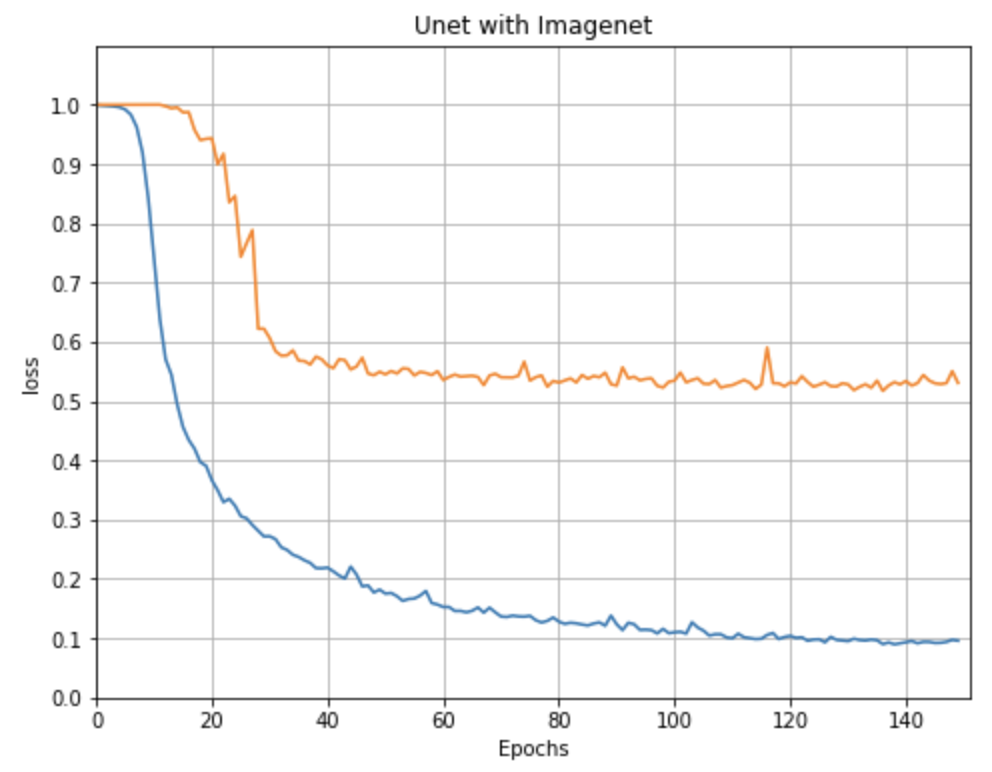
\includegraphics[width=\linewidth]{Materials/Method/UnetImagenet}
%		\caption{Model weights initialized with ImageNet weights.}
%	\end{subfigure}
%	\begin{subfigure}[b]{0.48\linewidth}
%		\centering
%		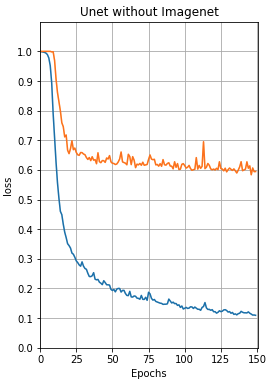
\includegraphics[width=\linewidth]{Materials/Method/UnetNoImagenet}
%		\caption{Model weights not initialized with ImageNet weights.}
%	\end{subfigure}
%	\caption{Both models are trained on unmodified training data. The blue graphs indicates training loss measured with DICE, and the orange graphs indicates validation loss also measured with DICE.}
%	\label{imagenet}
%\end{figure}

\subsection{Testing}
To measure the models unbiased performance on unknown data, the test set is used. As all predictions and true masks have image sizes 524 x 544 they are resized back to original sizes using the same interpolation rules. The 'immediate' output of the models are confidence maps, and to make these binary, we threshold them. This is done by thresholding all predicted masks from the training set and then computing the average DICE. The threshold that achieves the highest average DICE is then chosen, and all predicted masks from the test set are then thresholded by this value, and its unbiased performance can then be measured.\\
There exists different ways of measuring DICE on the test set. The test set can be split into three separate volumes, one for the single series images, one for the five series images and one for the six series images and the average DICE can then be measured across each. The three volumes can also further be split into 'time intervals' where the DICE is measured across all the images coming first in the series, second in the series and so on.

\subsection{Augmentations}
The first augmentation used is large random rotations. Here each of the original images have been rotated between $-45$ and $45$ degrees. Another dataset of small random rotations between $-30$ and $30$ degrees have also been created. The next augmentations flips each image horizontally and vertically giving us two more datasets. Two datasets have also been created for small and large random shearing in both the \textit{x} and \textit{y} direction. A \textit{mix} dataset has also been created where the original images were first sheared then rotated and finally flipped horizontally. A dataset was also created where the original images were 'bend' around the middle to form an arc shape. The last dataset created used the python package \textit{imgaug} to randomly apply one or more of the following augmentations to each image: horizontal flipping, vertical flipping, $80-120\%$ scaling, small translations, $-45$ to $45$ degrees rotations, $-16$ to $16$ degrees shearing, randomly drop $1-10\%$ of the pixels in the image, locally move some pixels around and lastly, perform local distortions. 

\subsection{Construction of augmented training sets}\label{construction}
With the augmented datasets, several training sets were constructed and used to train models. Each training set consists of 506 training images, and is constructed by randomly sample from the involved datasets without replacement, ensuring an even amount of images are taken from each dataset. An \textit{original} training set is also created consisting of the un-augmented images.
\section{Results}
In this section the results of the thesis work is presented. First we will take a look at some examples images from two endoscopy videos to familiarize ourselves a little with the data the models have been trained on. We will then look at the model selection and how the best performing model was chosen, followed by the separation point predictions of the post-processing approaches. Next we look at the treatment predictions from the segmentation results of the 2D ResNet, before we try and refine these results by a using U-Net model. To end with, we use the U-Net segmentations for treatment predictions. 

In \autoref{exampleFrames} we see four examples of training data from two different endoscopy videos and two different patients. In the left column we have examples of inflamed bowel tissue and in the right column examples of healthy bowel tissue. The top row of images is from the same video and likewise, the bottom row of images is from the same video. We note how even though the image pairs comes from the same patient, the colouring of the bowel tissue can change quite a lot throughout a video, which especially is seen in the bottom row of images. We also note, how much the colon twists has a large impact on the lighting, and thus on the colouring of the tissue. And lastly we also see from image (a) and (d) how similar healthy and inflamed tissue can look. 

\begin{figure}[H]
	\centering
	\begin{subfigure}{0.4\linewidth}
		\centering
		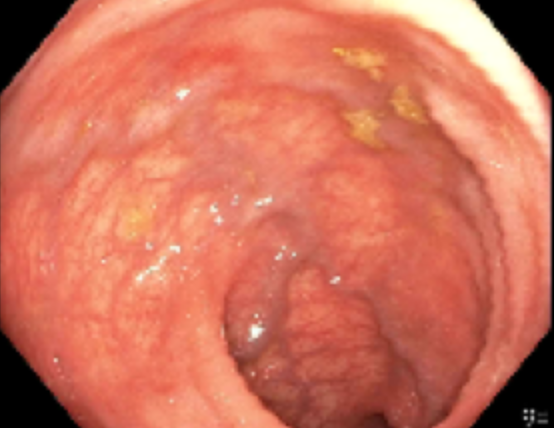
\includegraphics[width=\linewidth]{Materials/Results/Intro/idx_1_frame_830}
		\caption{Inflamed example image from validation video.}
	\end{subfigure}
	\hspace{0.5cm}
	\begin{subfigure}{0.4\linewidth}
		\centering
		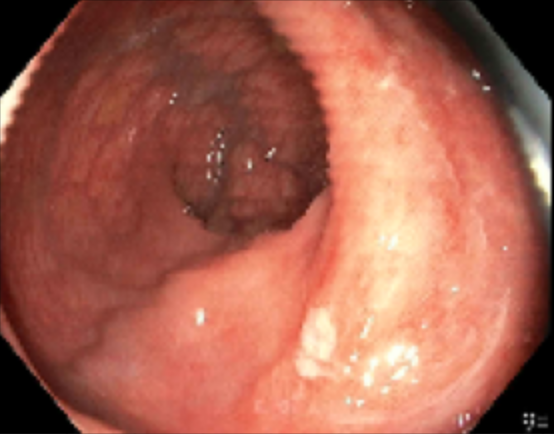
\includegraphics[width=\linewidth]{Materials/Results/Intro/idx_1_frame_1210}
		\caption{Healthy example image from validation video.\newline}
	\end{subfigure}
	\\
	\begin{subfigure}{0.4\linewidth}
		\centering
		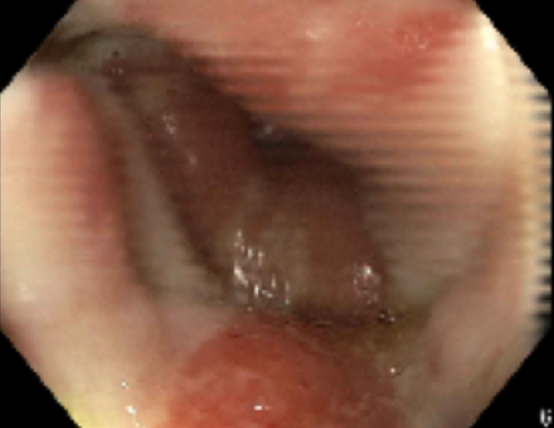
\includegraphics[width=\linewidth]{Materials/Results/Intro/idx_4_frame_800}
		\caption{Inflamed example image.}
	\end{subfigure}
	\hspace{0.5cm}
	\begin{subfigure}{0.4\linewidth}
		\centering
		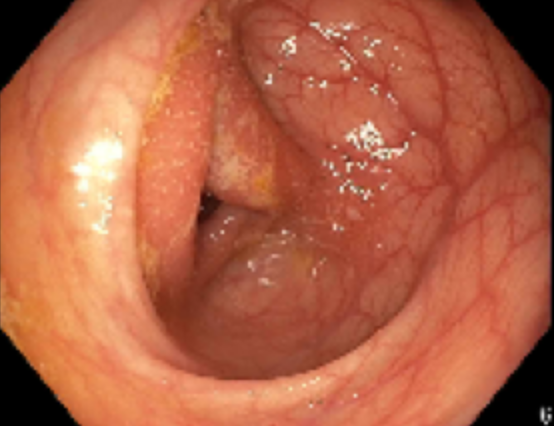
\includegraphics[width=\linewidth]{Materials/Results/Intro/idx_4_frame_3000}
		\caption{Healthy example image.}
	\end{subfigure}
	\caption{Examples images from two endoscopy videos.}
	\label{exampleFrames}
\end{figure}

\subsection{Model evaluation and selection} \label{modelRes}
Training was conducted by training several 2D ResNet models, one for each of the datasets, and using a single video as a constant validation set to tune learning rate, weight decay and the dropout layers. For loss functions binary cross entropy was used and for optimization Adam was used. Each model was trained for 65 epochs with a learning rate of $10^{-5}$. No weight decay was added. The true segmentations was 'artificially' constructed by concatenating a vector of zeros equal in length to the number of frames up to the true separation point, and a vector of ones equal in length to the remaining frames of the video, such that we get one continuous block of inflammation predictions followed by one continuous block of healthy predictions which correspond to how the doctor annotated the video.\\ 
In this section two results will be reported. First a five fold approach used to evaluate the model performance where each dataset is split in five folds, then a model is trained on four folds and evaluated on the constant validation set. Second, models are trained on all the data from each dataset respectively, and then used to predict each frame in the validation set for visual inspection.

\begin{table}[H]
	\hspace{-2.2cm}
	\begin{tabular}{|l|cc|cc|cc|cc|cc|r|r|r|}
		\hline
		\multicolumn{1}{|c|}{Dataset}    & \multicolumn{2}{c|}{Fold 1}                                                                                                     & \multicolumn{2}{c|}{Fold 2}                                                                                                     & \multicolumn{2}{c|}{Fold 3}                                                                                                     & \multicolumn{2}{c|}{Fold 4}                                                                                                     & \multicolumn{2}{c|}{Fold 5}                                                                                                     & \multicolumn{1}{c|}{Avg. T}           & \multicolumn{1}{c|}{Avg. V}           & \multicolumn{1}{c|}{Frames} \\ \hline
		\multicolumn{1}{|c|}{}           & \multicolumn{1}{c|}{T}                                                    & V                                                   & \multicolumn{1}{c|}{T}                                                    & V                                                   & \multicolumn{1}{c|}{T}                                                    & V                                                   & \multicolumn{1}{c|}{T}                                                    & V                                                   & \multicolumn{1}{c|}{T}                                                    & V                                                   & \multicolumn{1}{l|}{}                 & \multicolumn{1}{l|}{}                 & \multicolumn{1}{l|}{}       \\ \hline
		Idx\_4\_skip\_10                 & \multicolumn{1}{c|}{\cellcolor[HTML]{FFC7CE}{\color[HTML]{9C0006} 100.0}} & \cellcolor[HTML]{C6EFCE}{\color[HTML]{006100} 67.9} & \multicolumn{1}{c|}{\cellcolor[HTML]{FFC7CE}{\color[HTML]{9C0006} 100.0}} & \cellcolor[HTML]{C6EFCE}{\color[HTML]{006100} 33.2} & \multicolumn{1}{c|}{\cellcolor[HTML]{FFC7CE}{\color[HTML]{9C0006} 100.0}} & \cellcolor[HTML]{C6EFCE}{\color[HTML]{006100} 35.5} & \multicolumn{1}{c|}{\cellcolor[HTML]{FFC7CE}{\color[HTML]{9C0006} 100.0}} & \cellcolor[HTML]{C6EFCE}{\color[HTML]{006100} 43.1} & \multicolumn{1}{c|}{\cellcolor[HTML]{FFC7CE}{\color[HTML]{9C0006} 100.0}} & \cellcolor[HTML]{C6EFCE}{\color[HTML]{006100} 45.9} & {\color[HTML]{7F7F7F} \textit{100}}   & {\color[HTML]{7F7F7F} \textit{45.12}} & 499                         \\ \hline
		Idx\_4\_5\_skip\_20              & \multicolumn{1}{c|}{\cellcolor[HTML]{FFC7CE}{\color[HTML]{9C0006} 99.2}}  & \cellcolor[HTML]{C6EFCE}{\color[HTML]{006100} 47.2} & \multicolumn{1}{c|}{\cellcolor[HTML]{FFC7CE}{\color[HTML]{9C0006} 100.0}} & \cellcolor[HTML]{C6EFCE}{\color[HTML]{006100} 41.0} & \multicolumn{1}{c|}{\cellcolor[HTML]{FFC7CE}{\color[HTML]{9C0006} 99.8}}  & \cellcolor[HTML]{C6EFCE}{\color[HTML]{006100} 35.6} & \multicolumn{1}{c|}{\cellcolor[HTML]{FFC7CE}{\color[HTML]{9C0006} 100.0}} & \cellcolor[HTML]{C6EFCE}{\color[HTML]{006100} 39.0} & \multicolumn{1}{c|}{\cellcolor[HTML]{FFC7CE}{\color[HTML]{9C0006} 99.5}}  & \cellcolor[HTML]{C6EFCE}{\color[HTML]{006100} 33.0} & {\color[HTML]{7F7F7F} \textit{99.7}}  & {\color[HTML]{7F7F7F} \textit{39.16}} & 500                         \\ \hline
		Idx\_2\_3\_4\_5\_6\_skip\_50     & \multicolumn{1}{c|}{\cellcolor[HTML]{FFC7CE}{\color[HTML]{9C0006} 99.5}}  & \cellcolor[HTML]{C6EFCE}{\color[HTML]{006100} 71.4} & \multicolumn{1}{c|}{\cellcolor[HTML]{FFC7CE}{\color[HTML]{9C0006} 99.5}}  & \cellcolor[HTML]{C6EFCE}{\color[HTML]{006100} 63.7} & \multicolumn{1}{c|}{\cellcolor[HTML]{FFC7CE}{\color[HTML]{9C0006} 99.5}}  & \cellcolor[HTML]{C6EFCE}{\color[HTML]{006100} 70.0} & \multicolumn{1}{c|}{\cellcolor[HTML]{FFC7CE}{\color[HTML]{9C0006} 99.7}}  & \cellcolor[HTML]{C6EFCE}{\color[HTML]{006100} 45.5} & \multicolumn{1}{c|}{\cellcolor[HTML]{FFC7CE}{\color[HTML]{9C0006} 100.0}} & \cellcolor[HTML]{C6EFCE}{\color[HTML]{006100} 43.4} & {\color[HTML]{7F7F7F} \textit{99.64}} & {\color[HTML]{7F7F7F} \textit{58.8}}  & 491                         \\ \hline
		Idx\_2\_3\_4\_5\_6\_skip\_20     & \multicolumn{1}{c|}{\cellcolor[HTML]{FFC7CE}{\color[HTML]{9C0006} 100.0}} & \cellcolor[HTML]{C6EFCE}{\color[HTML]{006100} 60.9} & \multicolumn{1}{c|}{\cellcolor[HTML]{FFC7CE}{\color[HTML]{9C0006} 99.7}}  & \cellcolor[HTML]{C6EFCE}{\color[HTML]{006100} 61.8} & \multicolumn{1}{c|}{\cellcolor[HTML]{FFC7CE}{\color[HTML]{9C0006} 99.7}}  & \cellcolor[HTML]{C6EFCE}{\color[HTML]{006100} 66.2} & \multicolumn{1}{c|}{\cellcolor[HTML]{FFC7CE}{\color[HTML]{9C0006} 99.7}}  & \cellcolor[HTML]{C6EFCE}{\color[HTML]{006100} 71.4} & \multicolumn{1}{c|}{\cellcolor[HTML]{FFC7CE}{\color[HTML]{9C0006} 99.8}}  & \cellcolor[HTML]{C6EFCE}{\color[HTML]{006100} 65.5} & {\color[HTML]{7F7F7F} \textit{99.78}} & {\color[HTML]{7F7F7F} \textit{65.16}} & 1226                        \\ \hline
		Idx\_4\_14\_18\_20\_32\_skip\_20 & \multicolumn{1}{c|}{\cellcolor[HTML]{FFC7CE}{\color[HTML]{9C0006} 99.7}}  & \cellcolor[HTML]{C6EFCE}{\color[HTML]{006100} 33.9} & \multicolumn{1}{c|}{\cellcolor[HTML]{FFC7CE}{\color[HTML]{9C0006} 100.0}} & \cellcolor[HTML]{C6EFCE}{\color[HTML]{006100} 42.6} & \multicolumn{1}{c|}{\cellcolor[HTML]{FFC7CE}{\color[HTML]{9C0006} 99.9}}  & \cellcolor[HTML]{C6EFCE}{\color[HTML]{006100} 40.6} & \multicolumn{1}{c|}{\cellcolor[HTML]{FFC7CE}{\color[HTML]{9C0006} 99.9}}  & \cellcolor[HTML]{C6EFCE}{\color[HTML]{006100} 37.2} & \multicolumn{1}{c|}{\cellcolor[HTML]{FFC7CE}{\color[HTML]{9C0006} 99.8}}  & \cellcolor[HTML]{C6EFCE}{\color[HTML]{006100} 38.2} & {\color[HTML]{7F7F7F} \textit{99.86}} & {\color[HTML]{7F7F7F} \textit{38.5}}  & 997                         \\ \hline
		Idx\_4\_14\_18\_20\_32\_skip\_5  & \multicolumn{1}{c|}{\cellcolor[HTML]{FFC7CE}{\color[HTML]{9C0006} 99.9}}  & \cellcolor[HTML]{C6EFCE}{\color[HTML]{006100} 69.3} & \multicolumn{1}{c|}{\cellcolor[HTML]{FFC7CE}{\color[HTML]{9C0006} 100.0}} & \cellcolor[HTML]{C6EFCE}{\color[HTML]{006100} 57.1} & \multicolumn{1}{c|}{\cellcolor[HTML]{FFC7CE}{\color[HTML]{9C0006} 86.4}}  & \cellcolor[HTML]{C6EFCE}{\color[HTML]{006100} 39.5} & \multicolumn{1}{c|}{\cellcolor[HTML]{FFC7CE}{\color[HTML]{9C0006} 99.5}}  & \cellcolor[HTML]{C6EFCE}{\color[HTML]{006100} 55.9} & \multicolumn{1}{c|}{\cellcolor[HTML]{FFC7CE}{\color[HTML]{9C0006} 99.9}}  & \cellcolor[HTML]{C6EFCE}{\color[HTML]{006100} 60.9} & {\color[HTML]{7F7F7F} \textit{97.14}} & {\color[HTML]{7F7F7F} \textit{56.54}} & 3978                        \\ \hline
		Idx\_3\_23\_skip\_10             & \multicolumn{1}{c|}{\cellcolor[HTML]{FFC7CE}{\color[HTML]{9C0006} 100.0}} & \cellcolor[HTML]{C6EFCE}{\color[HTML]{006100} 72.0} & \multicolumn{1}{c|}{\cellcolor[HTML]{FFC7CE}{\color[HTML]{9C0006} 100.0}} & \cellcolor[HTML]{C6EFCE}{\color[HTML]{006100} 72.3} & \multicolumn{1}{c|}{\cellcolor[HTML]{FFC7CE}{\color[HTML]{9C0006} 100.0}} & \cellcolor[HTML]{C6EFCE}{\color[HTML]{006100} 72.6} & \multicolumn{1}{c|}{\cellcolor[HTML]{FFC7CE}{\color[HTML]{9C0006} 100.0}} & \cellcolor[HTML]{C6EFCE}{\color[HTML]{006100} 72.4} & \multicolumn{1}{c|}{\cellcolor[HTML]{FFC7CE}{\color[HTML]{9C0006} 100.0}} & \cellcolor[HTML]{C6EFCE}{\color[HTML]{006100} 70.6} & {\color[HTML]{7F7F7F} \textit{100.0}} & {\color[HTML]{7F7F7F} \textit{72.0}}  & 829                         \\ \hline
		Idx\_19\_24\_skip\_5             & \multicolumn{1}{c|}{\cellcolor[HTML]{FFC7CE}{\color[HTML]{9C0006} 100.0}} & \cellcolor[HTML]{C6EFCE}{\color[HTML]{006100} 26.8} & \multicolumn{1}{c|}{\cellcolor[HTML]{FFC7CE}{\color[HTML]{9C0006} 100.0}} & \cellcolor[HTML]{C6EFCE}{\color[HTML]{006100} 25.9} & \multicolumn{1}{c|}{\cellcolor[HTML]{FFC7CE}{\color[HTML]{9C0006} 99.8}}  & \cellcolor[HTML]{C6EFCE}{\color[HTML]{006100} 27.7} & \multicolumn{1}{c|}{\cellcolor[HTML]{FFC7CE}{\color[HTML]{9C0006} 100.0}} & \cellcolor[HTML]{C6EFCE}{\color[HTML]{006100} 27.3} & \multicolumn{1}{c|}{\cellcolor[HTML]{FFC7CE}{\color[HTML]{9C0006} 100.0}} & \cellcolor[HTML]{C6EFCE}{\color[HTML]{006100} 26.7} & {\color[HTML]{7F7F7F} \textit{100.0}} & {\color[HTML]{7F7F7F} \textit{26.9}}  & 600                         \\ \hline
	\end{tabular}
	\caption{Evaluation results for training a modified 2D ResNet on different datasets. All results are in percent. At each fold, T stands for training accuracy and V stands for validation accuracy.}
	\label{2dresnetevalres}
\end{table}

In \autoref{2dresnetevalres} we see the evaluation of the five fold approach. T stands for training accuracy and V stands for validation accuracy. All results are reported in percent. We note dataset \textit{Idx\_3\_23\_skip\_10} and \textit{Idx\_2\_3\_4\_5\_6\_skip\_20} have the highest validation accuracies while \textit{Idx\_19\_24\_skip\_5} has the lowest followed by \textit{Idx\_4\_14\_18\_20\_32\_} \textit{skip\_5}. We also note there seemingly is no relation between the sheer number of training images and high validation accuracy, but there is some relation when we chose to add more images from the same dataset. Likewise there is seemingly no relation between the different number of patients the training images comes from and high validation accuracy.

To assert whether the reported accuracies are accurate, we will now take a look at how the models predicted on some videos. First we will look at how each of the models predicted on the validation video to establish a baseline. The results can be seen in \autoref{firstfive} and in \autoref{lastthree}. For each illustration the true segmentation of the video has been drawn as the first bar. For these results, this means approximately 72\% of the frames are annotated as inflamed and the last frames as healthy. The second bar is the model predictions. The blue line indicates the models' confidence in a healthy prediction, and a probability above 50\% means it has predicted the frame is healthy.

\begin{figure}[H]
	\centering
	\begin{subfigure}{\linewidth}
		\centering
		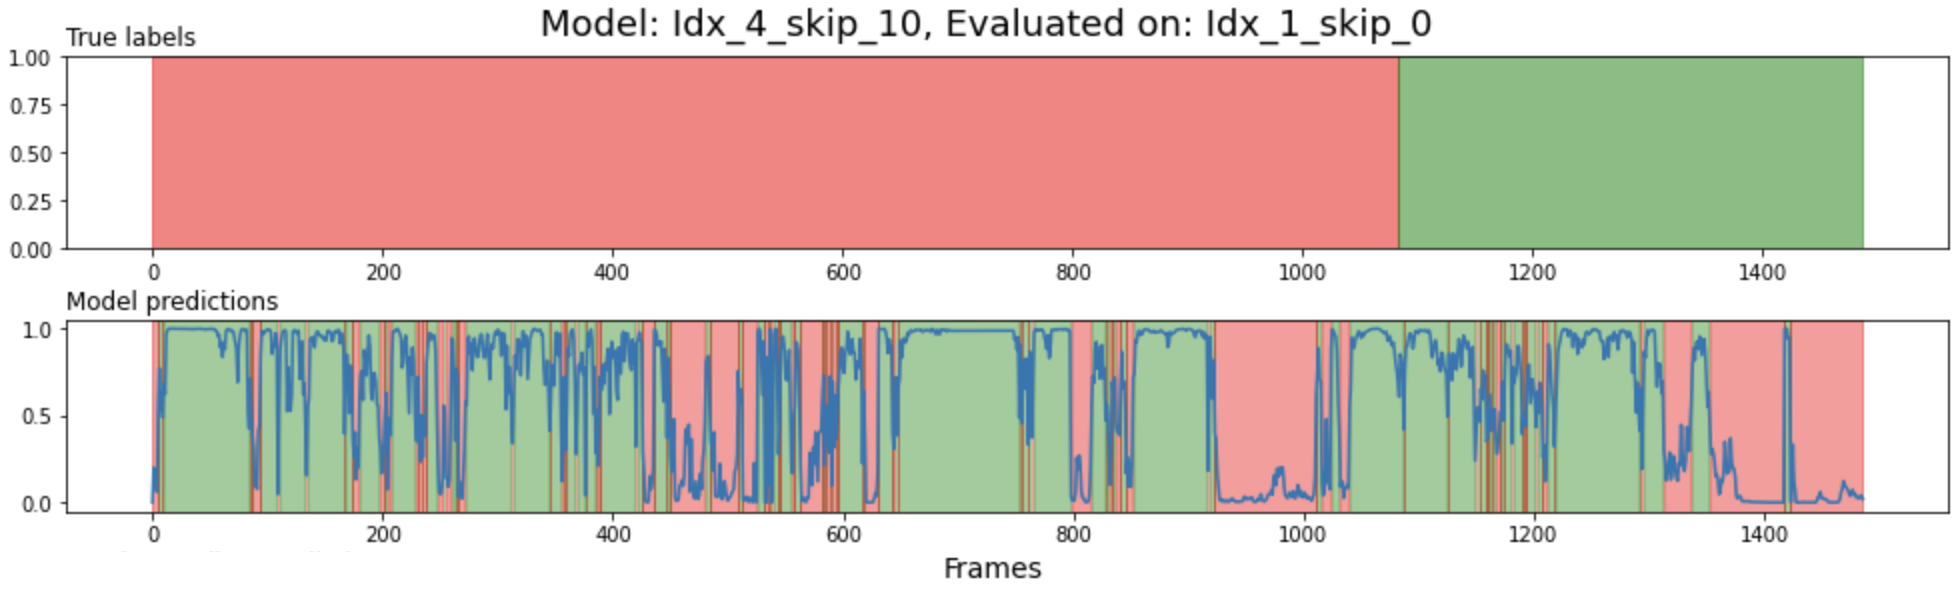
\includegraphics[width=\linewidth]{Materials/Results/SP/M1On1C}
	\end{subfigure}
	\\
	\begin{subfigure}{\linewidth}
		\centering
		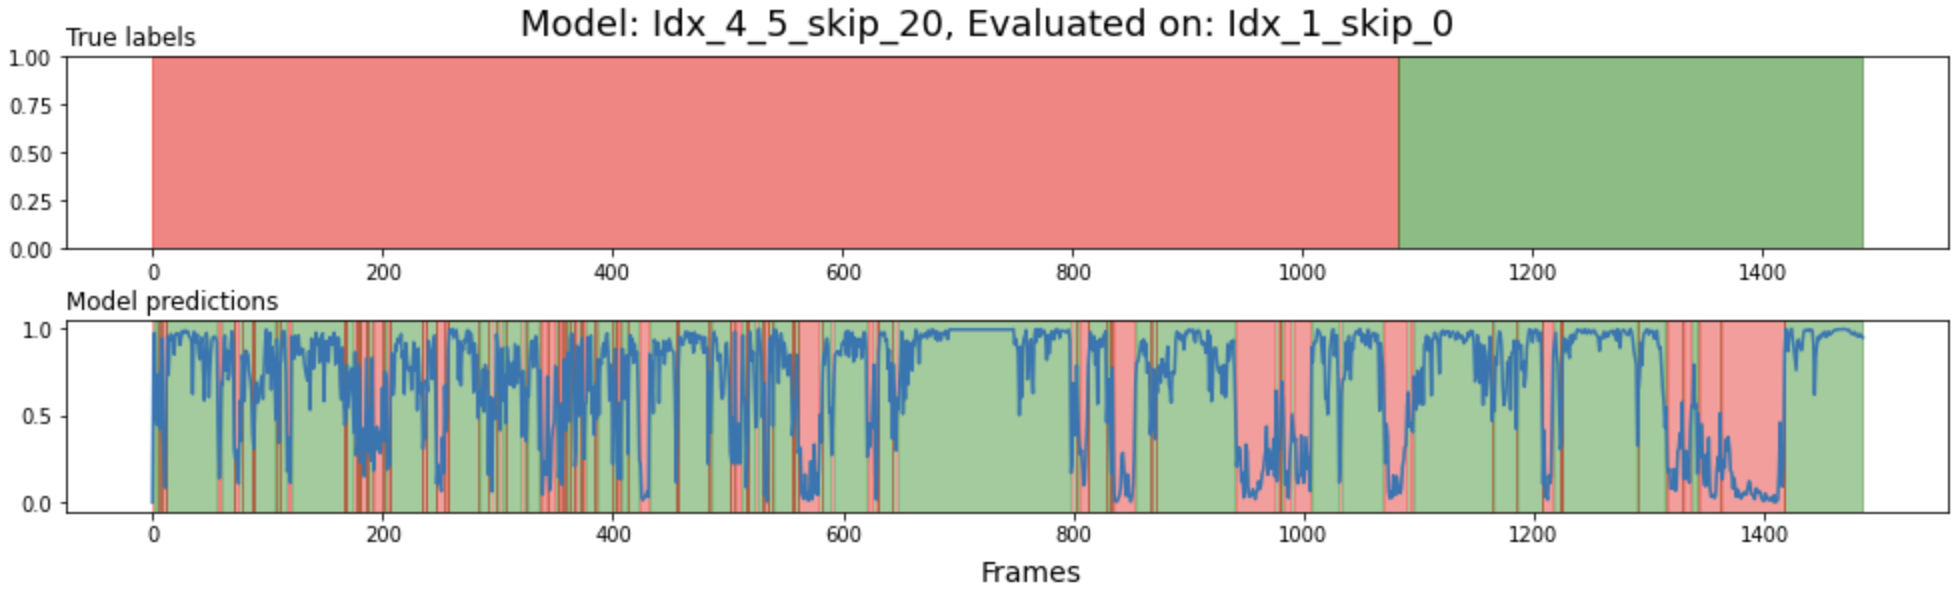
\includegraphics[width=\linewidth]{Materials/Results/SP/M2On1C}
	\end{subfigure}
	\\
	\begin{subfigure}{\linewidth}
		\centering
		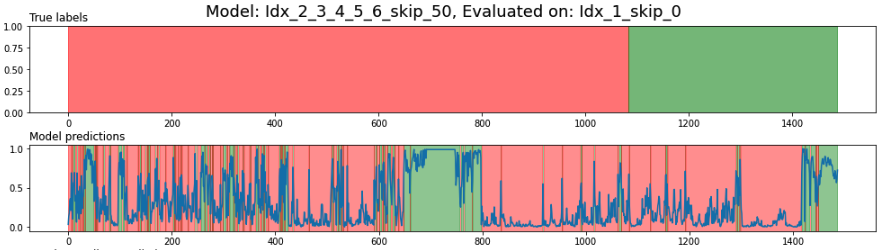
\includegraphics[width=\linewidth]{Materials/Results/SP/M3On1C}
	\end{subfigure}
	\\
	\begin{subfigure}{\linewidth}
		\centering
		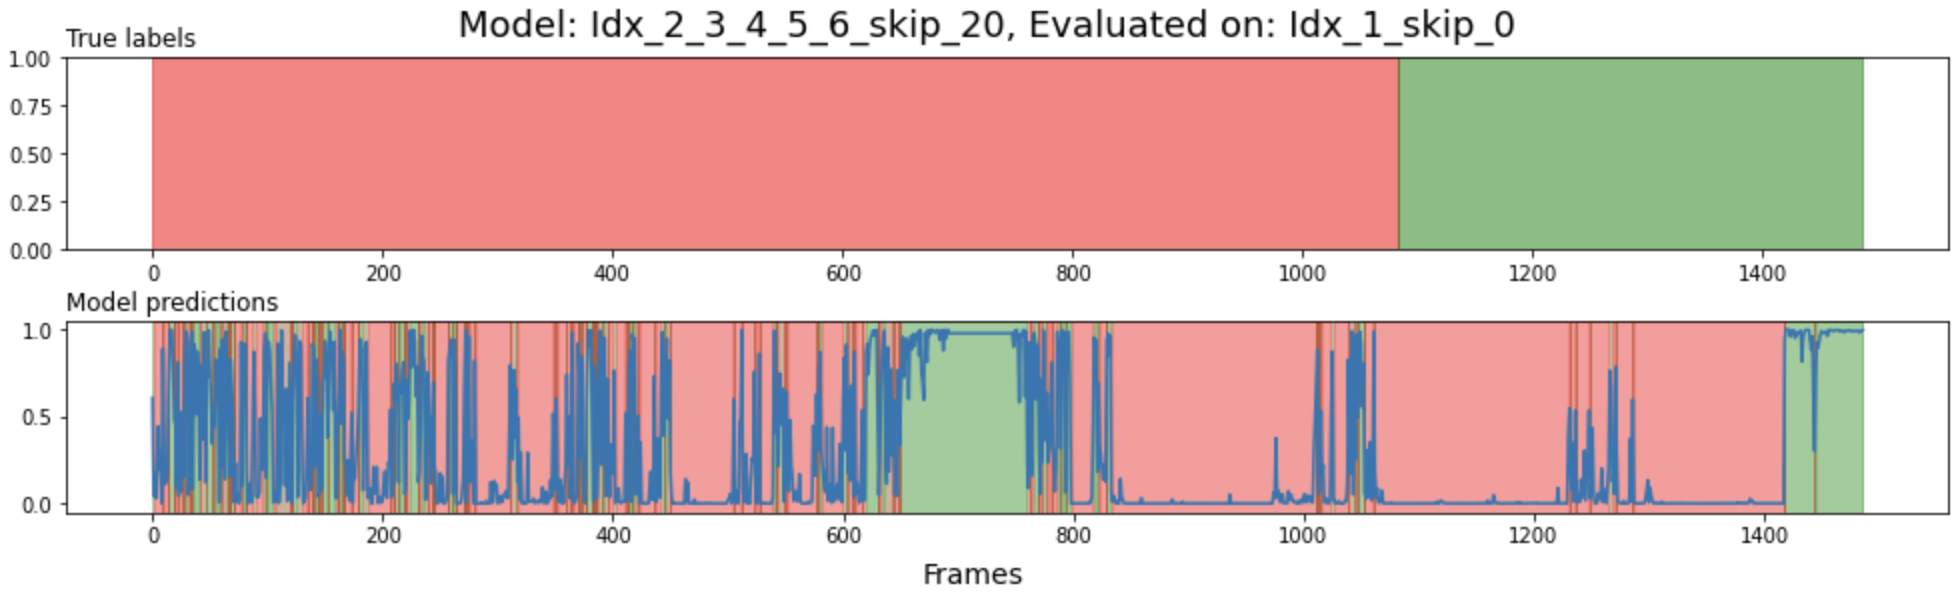
\includegraphics[width=\linewidth]{Materials/Results/SP/M4On1C}
	\end{subfigure}
	\\
	\begin{subfigure}{\linewidth}
		\centering
		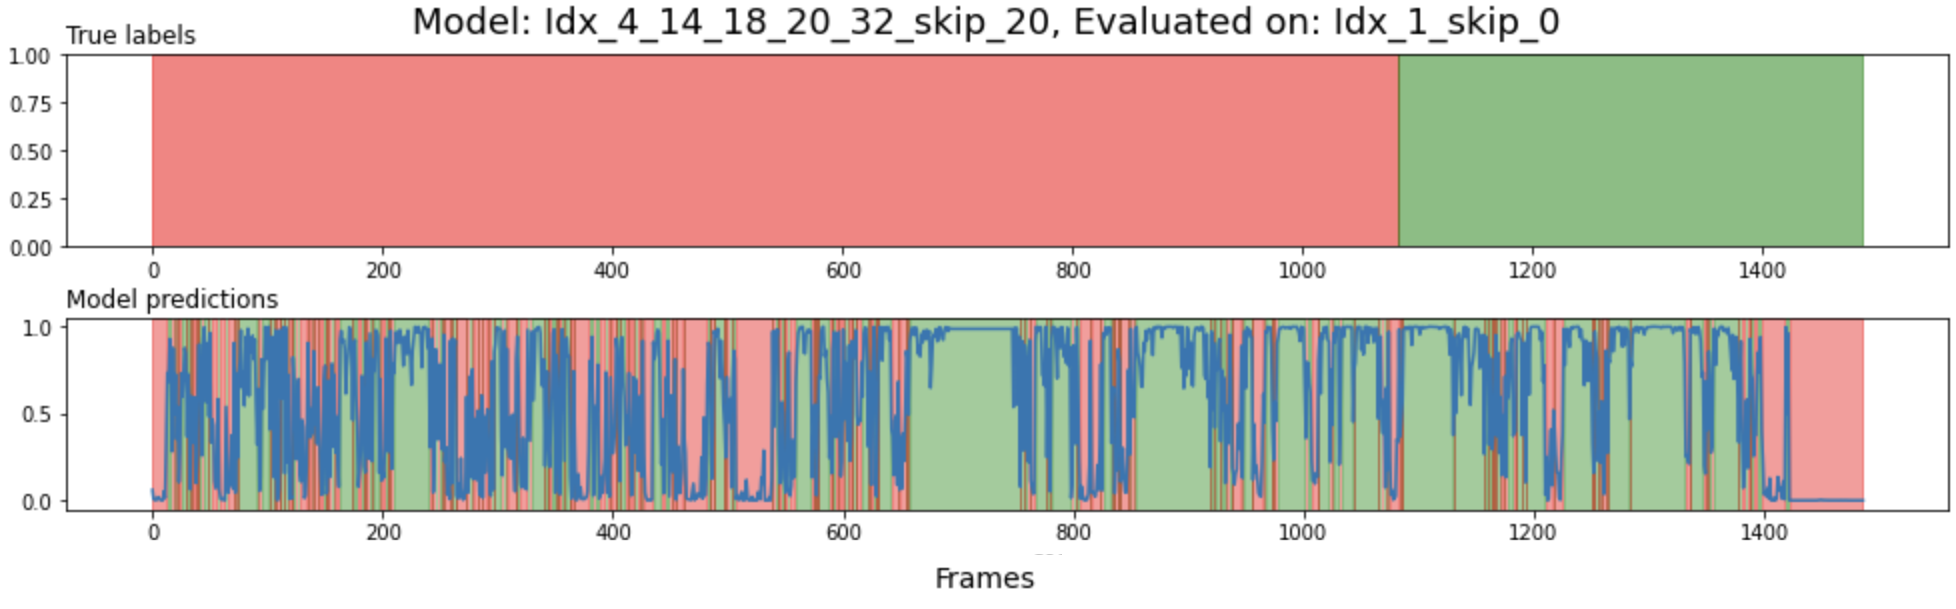
\includegraphics[width=\linewidth]{Materials/Results/SP/M5On1C}
	\end{subfigure}
	\caption{How the first five models predicted on the validation video.}
	\label{firstfive}
\end{figure}

\begin{figure}[H]
	\centering
	\begin{subfigure}{\linewidth}
		\centering
		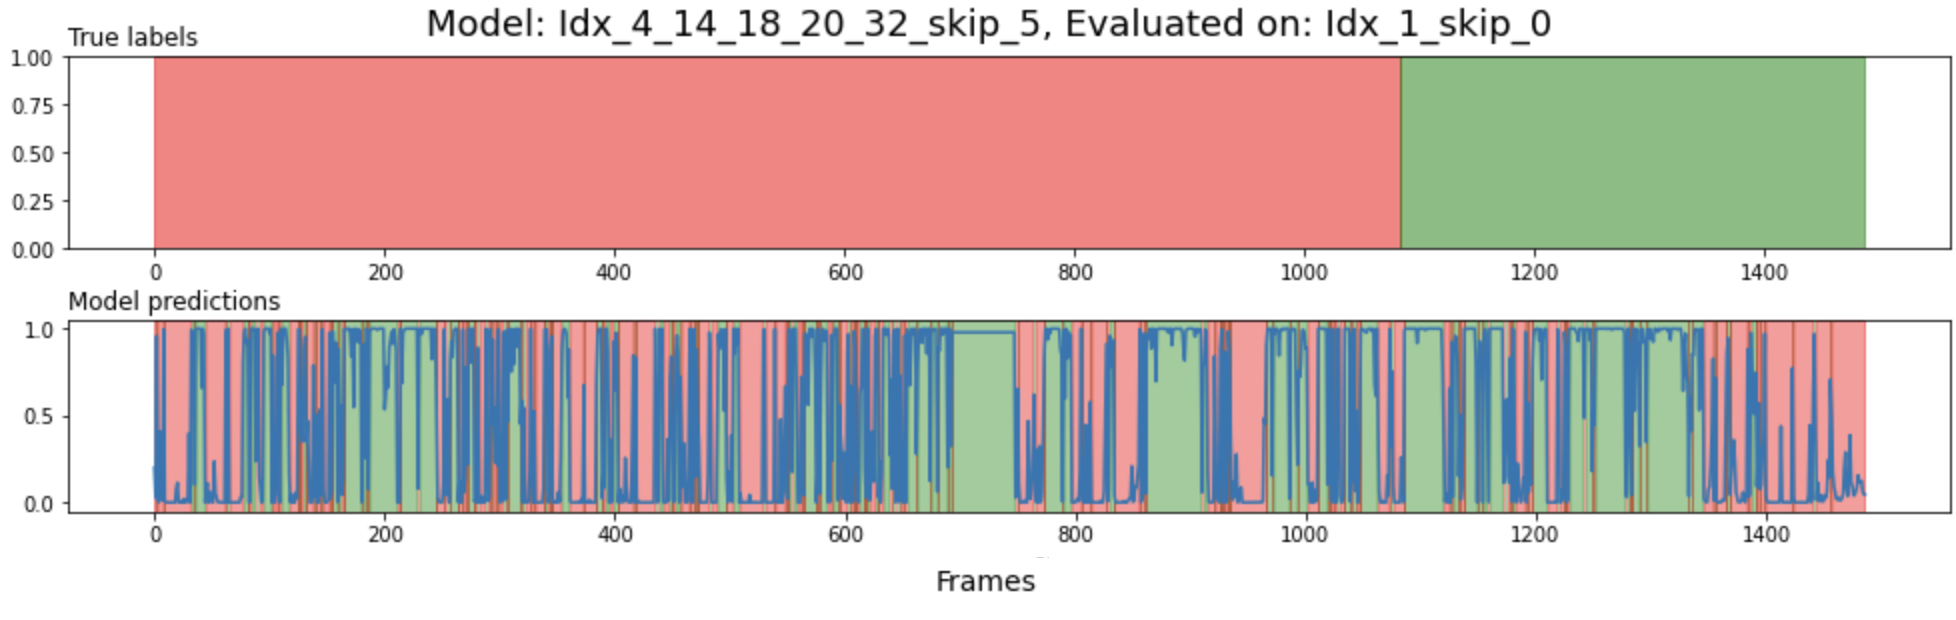
\includegraphics[width=\linewidth]{Materials/Results/SP/M6On1C}
	\end{subfigure}
	\\
	\begin{subfigure}{\linewidth}
		\centering
		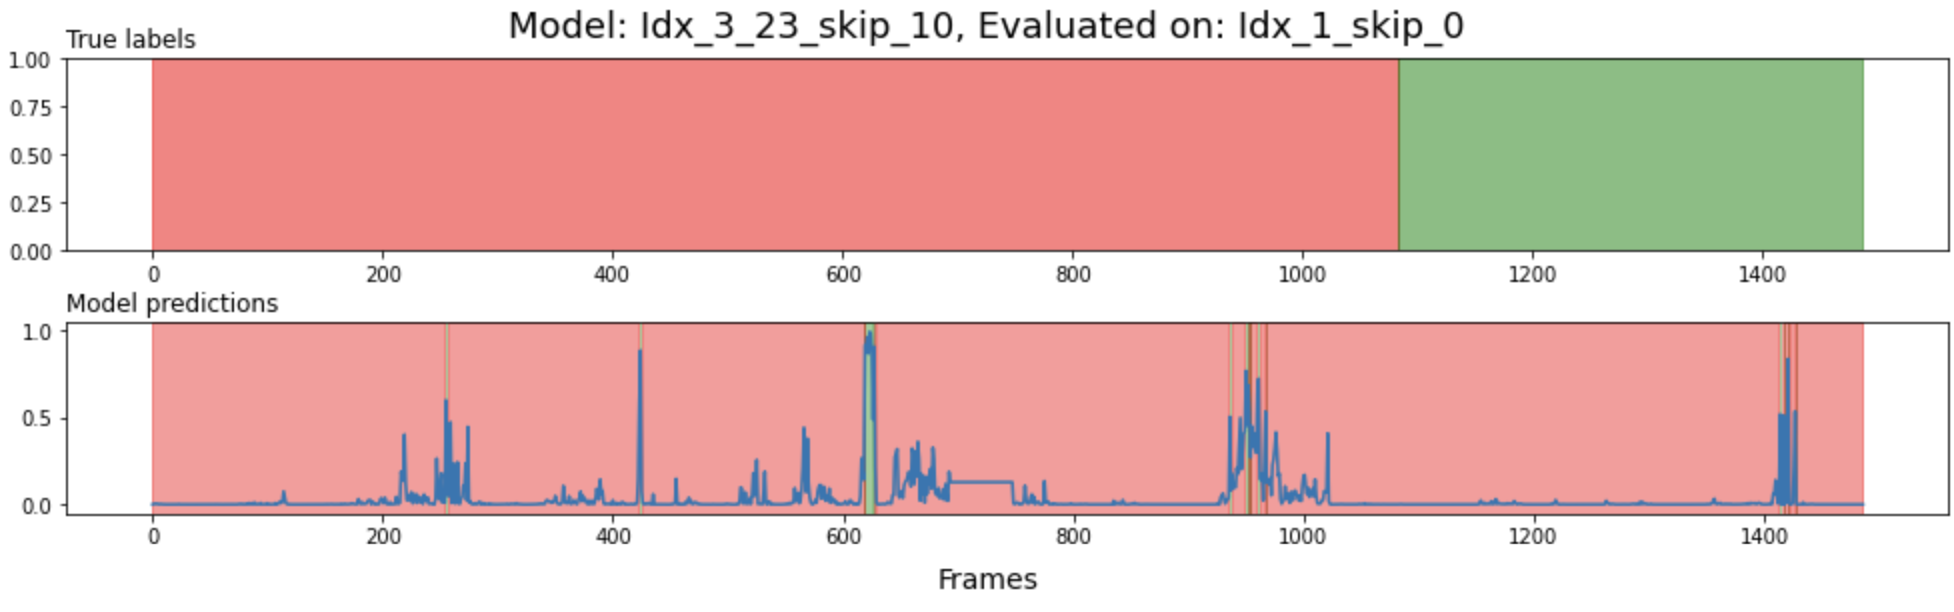
\includegraphics[width=\linewidth]{Materials/Results/SP/M7On1C}
	\end{subfigure}
	\\
	\begin{subfigure}{\linewidth}
		\centering
		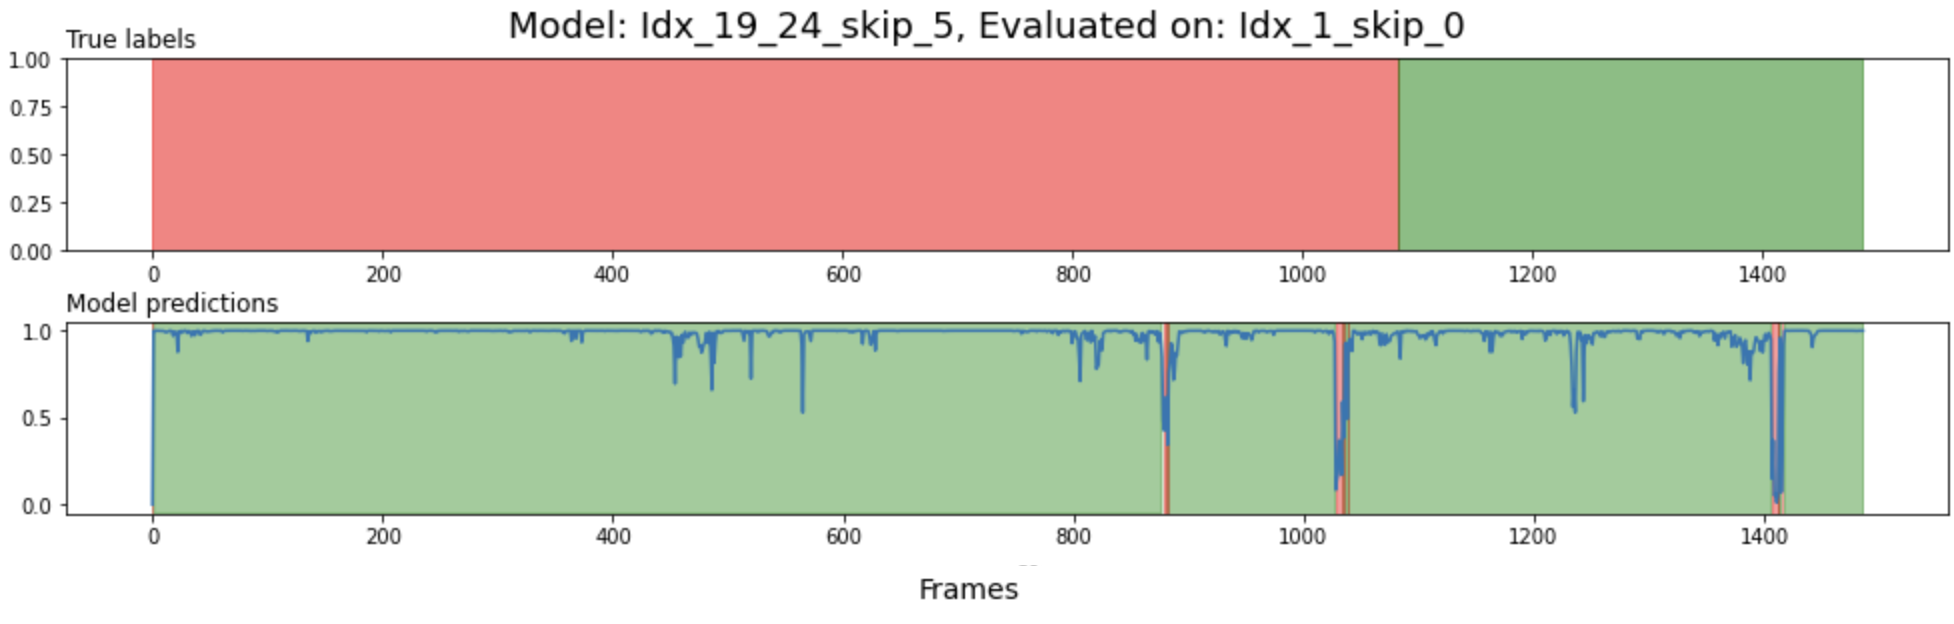
\includegraphics[width=\linewidth]{Materials/Results/SP/M8On1C}
	\end{subfigure}
	\caption{How the last three models predicted on the validation video.}
	\label{lastthree}
\end{figure}

We note how models \textit{Idx\_4\_skip\_10} and \textit{Idx\_4\_5\_skip\_20} predict overly many healthy frames but seem to be fairly confident in their predictions. Model \textit{Idx\_2\_3\_4\_5\_6\_skip\_50} have comparably predicted a lot more inflamed frames, but it still seem to be confident some of the first frames are healthy. Looking at model \textit{Idx\_2\_3\_4\_5\_6\_skip\_20} which scored the second highest validation accuracy, we see it has some rather volatile predictions on the early frames where most however seem to be classified as inflamed. On the other hand, it seem to predict quite confidently too many inflamed frames towards the end of the video. Model \textit{Idx\_4\_14\_18\_20\_32\_skip\_20} is the first model trained across several patients, but this models seem to predict a mix of the previous models as it has some volatile predictions in the beginning of the video, but towards the middle it begins to confidently predict overly many healthy frames. Model \textit{Idx\_4\_14\_18\_20\_32\_skip\_5} is the second model to be trained on several patients and also had a significant larger training set than the other models. Here we see only a few blocks of consecutive healthy predictions and otherwise some very volatile predictions. Towards the end of the video it predicts a large part correctly healthy, but it also predicts the very end inflamed. Model \textit{Idx\_3\_23\_skip\_10} was the model which achieved the highest validation accuracies, but we also see it very rarely predicts other than inflamed. As the validation video

\begin{figure}[H]
	\centering
	\begin{subfigure}{\linewidth}
		\centering
		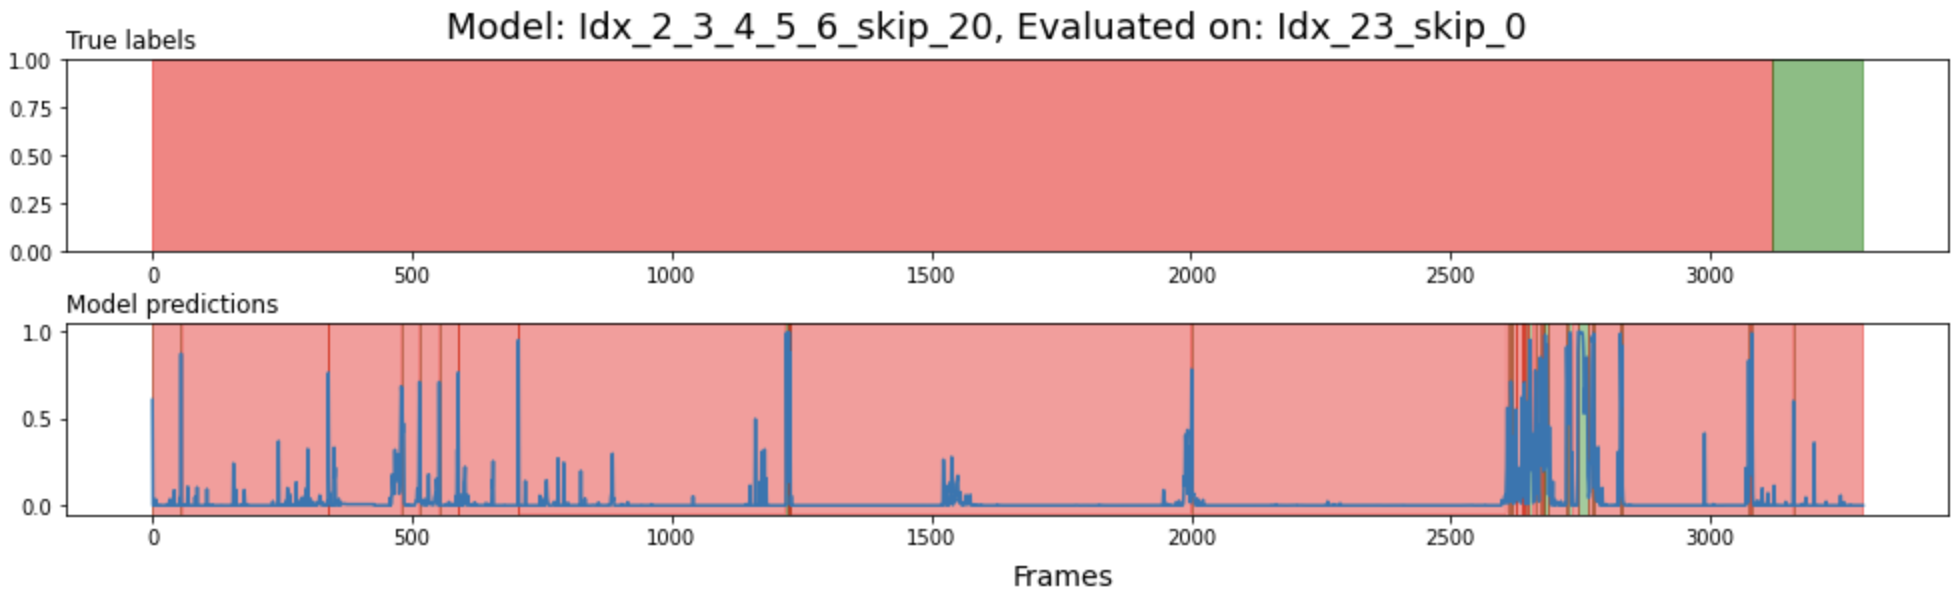
\includegraphics[width=\linewidth]{Materials/Results/SP/M4On23C}
	\end{subfigure}
	\\
	\begin{subfigure}{\linewidth}
		\centering
		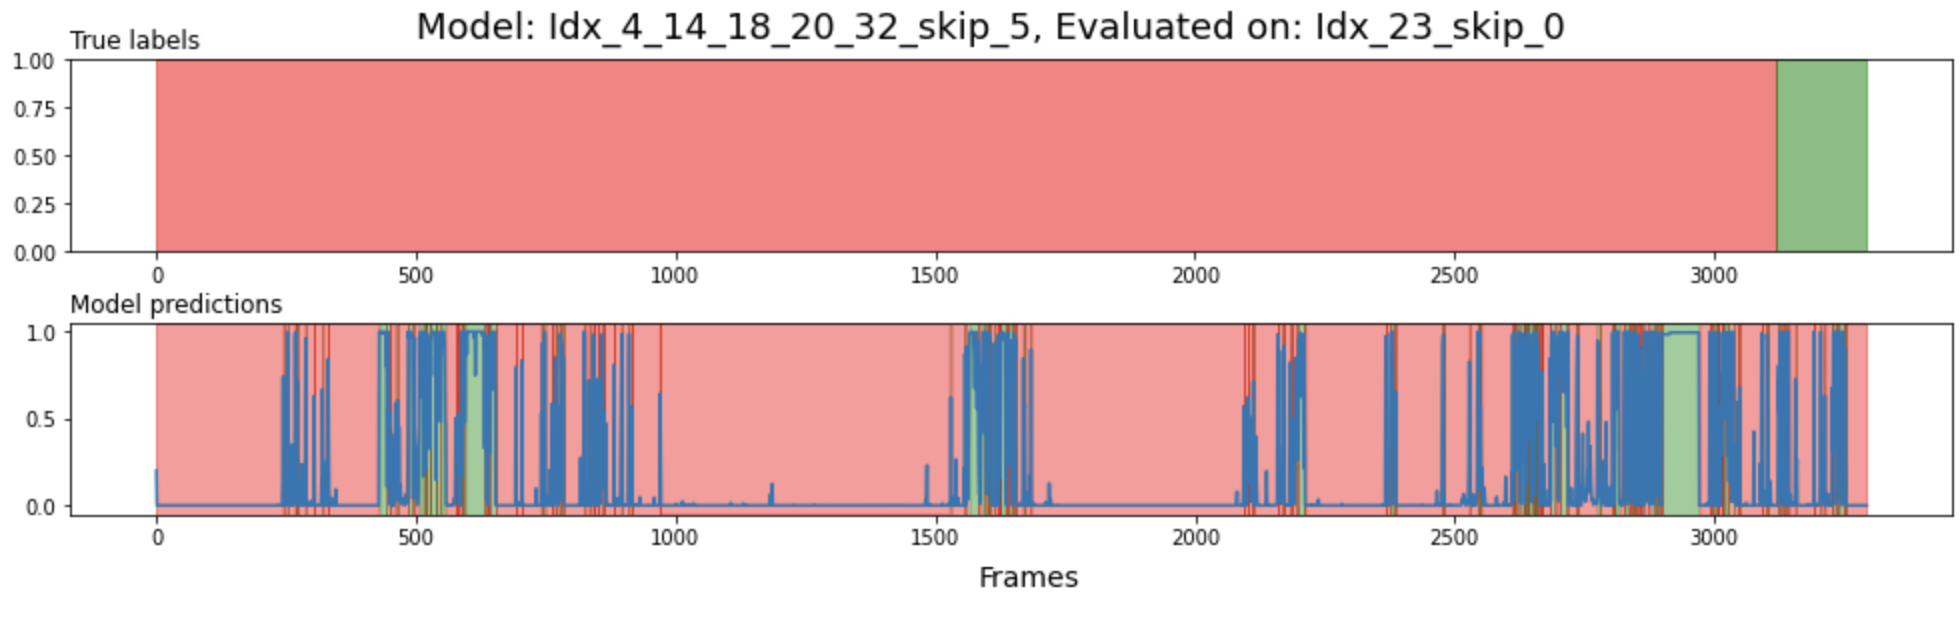
\includegraphics[width=\linewidth]{Materials/Results/SP/M6On23C}
	\end{subfigure}
	\caption{How the two selected models perform on test set \textit{Idx\_23\_skip\_0}.}
	\label{idx23}
\end{figure}

consists of approximately 72\% inflamed frames, it would seem its accuracy is skewed because of the imbalance in the data. Lastly we have model \textit{Idx\_19\_24\_skip\_5} which has the opposite issue where it only predicts healthy.

To select which model to move forward and perform treatment predictions with, models \textit{Idx\_2\_3\_4\_5\_6\_skip\_20} and \textit{Idx\_4\_14\_18\_20\_32\_skip\_5} were selected to predict on more videos. \textit{Idx\_2\_3\_4\_5\_6\_skip\_20} was selected as it seem to predict the best on the validation video and \textit{Idx\_4\_14\_18\_20\_32\_skip\_5} because prior knowledge say models trained on more and varied data should perform better, and thus we verify its validation results from \autoref{2dresnetevalres} are not amiss.

In \autoref{idx23} we see the predictions of the two models on an unseen video which is biased towards being inflamed. We see model \textit{Idx\_2\_3\_4\_5\_6\_skip\_20} predicting confidently and almost exclusively inflammation with a few healthy predictions in the wrong places. Model \textit{Idx\_4\_14\_18\_20\_32\_skip\_5} is more uncertain, and predicts healthy in some spots while having oscillating predictions. The largest consecutive part where it confidently predicts healthy is when it should have predicted inflammation.

In \autoref{idx24} we see the predictions of the two selected models on an unseen video biased towards being healthy. We see model \textit{Idx\_2\_3\_4\_5\_6\_skip\_20} still confidently predicting most frames inflamed, with a few correct exceptions towards the middle of the video. Model \textit{Idx\_4\_14\_18\_20\_32\_skip\_5} predicts most of the video inflamed too, but is not as certain and also correctly predicts one large block healthy.

As a last validation, in \autoref{idx28} we see the predictions of the two selected models on an unseen video biased towards inflammation. Model \textit{Idx\_2\_3\_4\_5\_6\_skip\_20} is rather volatile in its predictions at the beginning of the video, but seem to correctly predict mostly inflammation. Towards the end it seem to capture some of the healthy frames, but predicts a few too many. Model \textit{Idx\_4\_14\_18\_20\_32\_skip\_5} seems on the other hand very volatile, and seem to have some passages where it wrongly predicts healthy. Towards the end we still see some volatile predictions, but it does not seem to capture the healthy frames at the end.

\begin{figure}[H]
	\centering
	\begin{subfigure}{\linewidth}
		\centering
		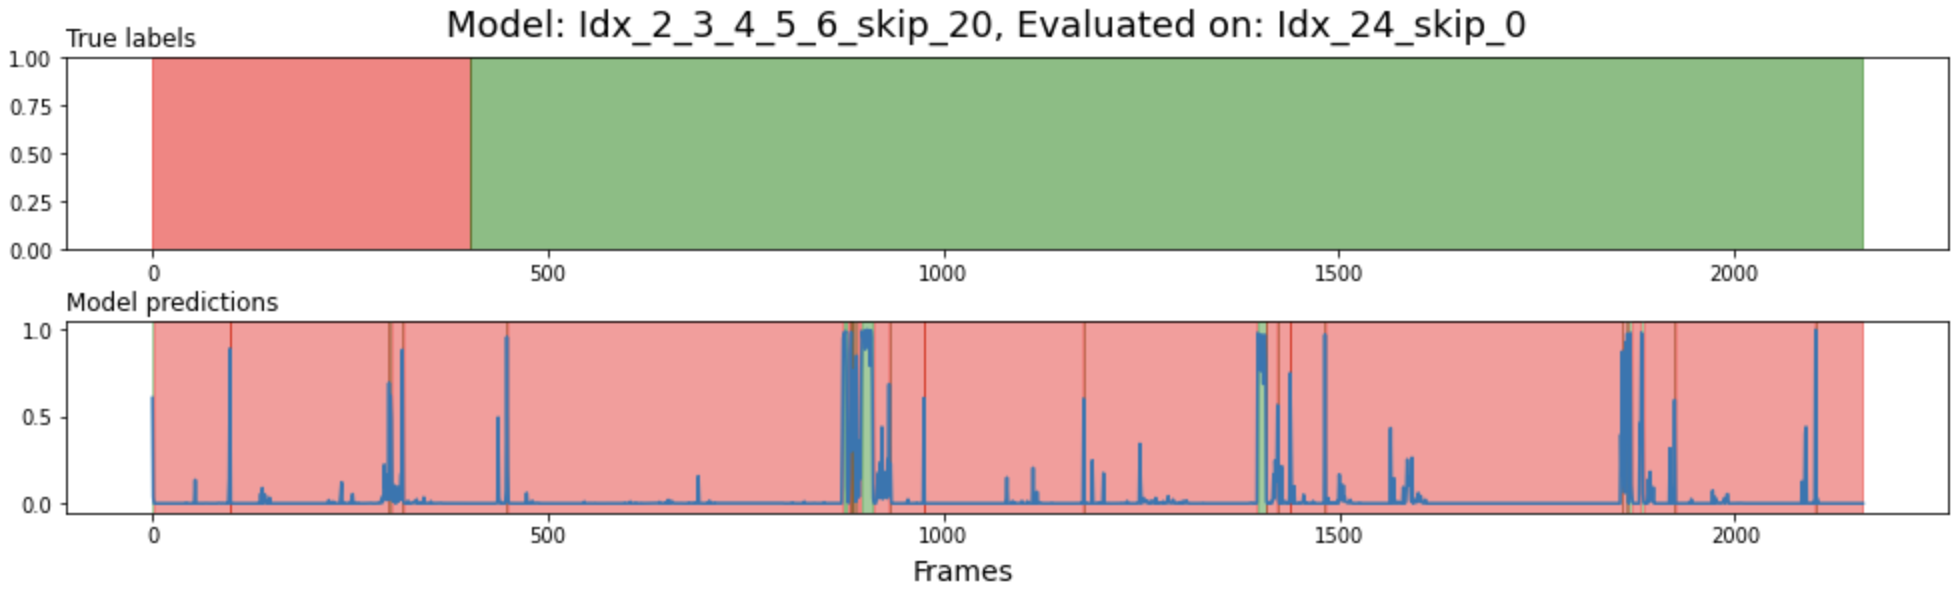
\includegraphics[width=\linewidth]{Materials/Results/SP/M4On24C}
	\end{subfigure}
	\\
	\begin{subfigure}{\linewidth}
		\centering
		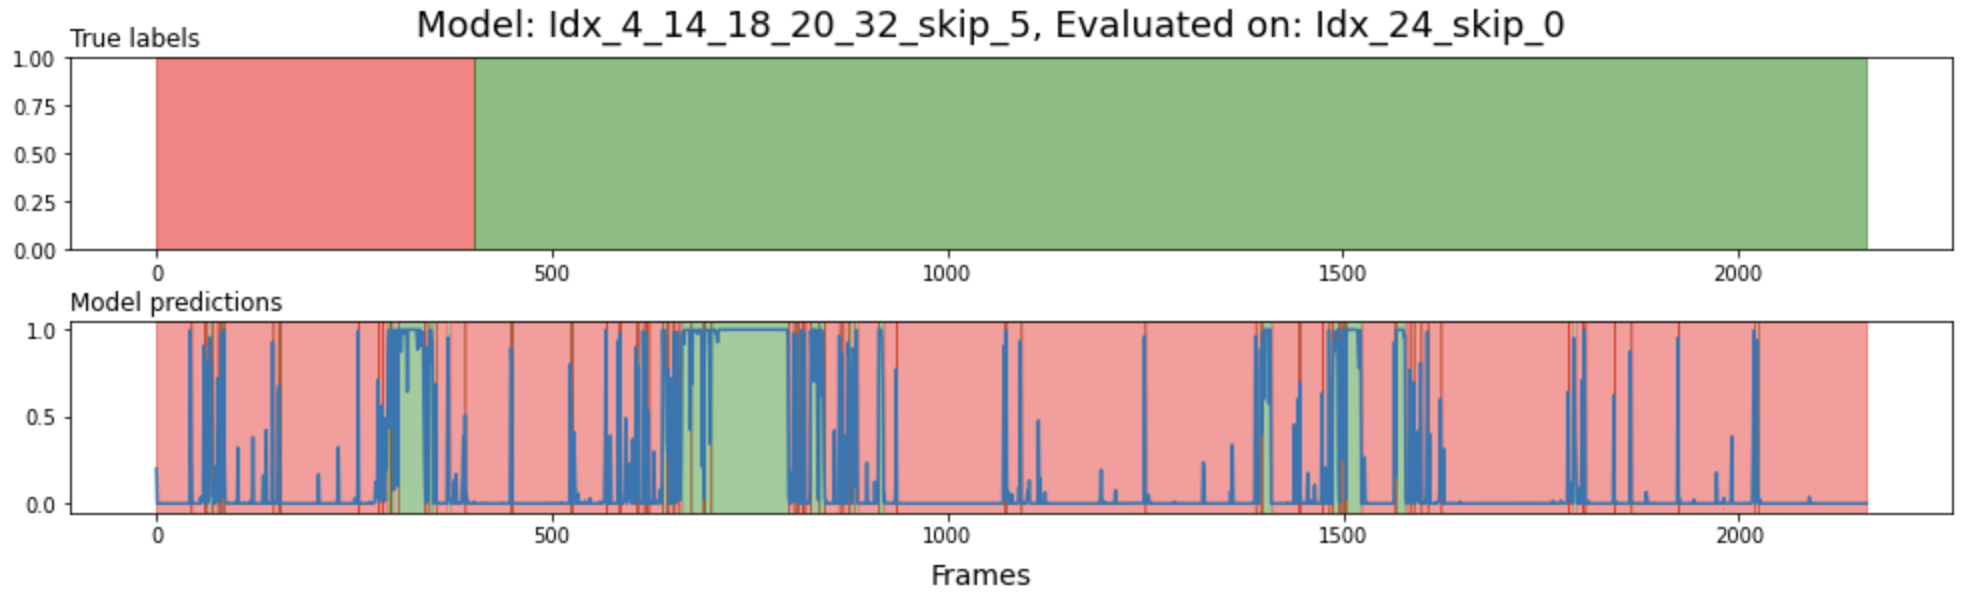
\includegraphics[width=\linewidth]{Materials/Results/SP/M6On24C}
	\end{subfigure}
	\caption{How the two selected models perform on test set \textit{Idx\_24\_skip\_0}.}
	\label{idx24}
\end{figure}

\begin{figure}[H]
	\centering
	\begin{subfigure}{\linewidth}
		\centering
		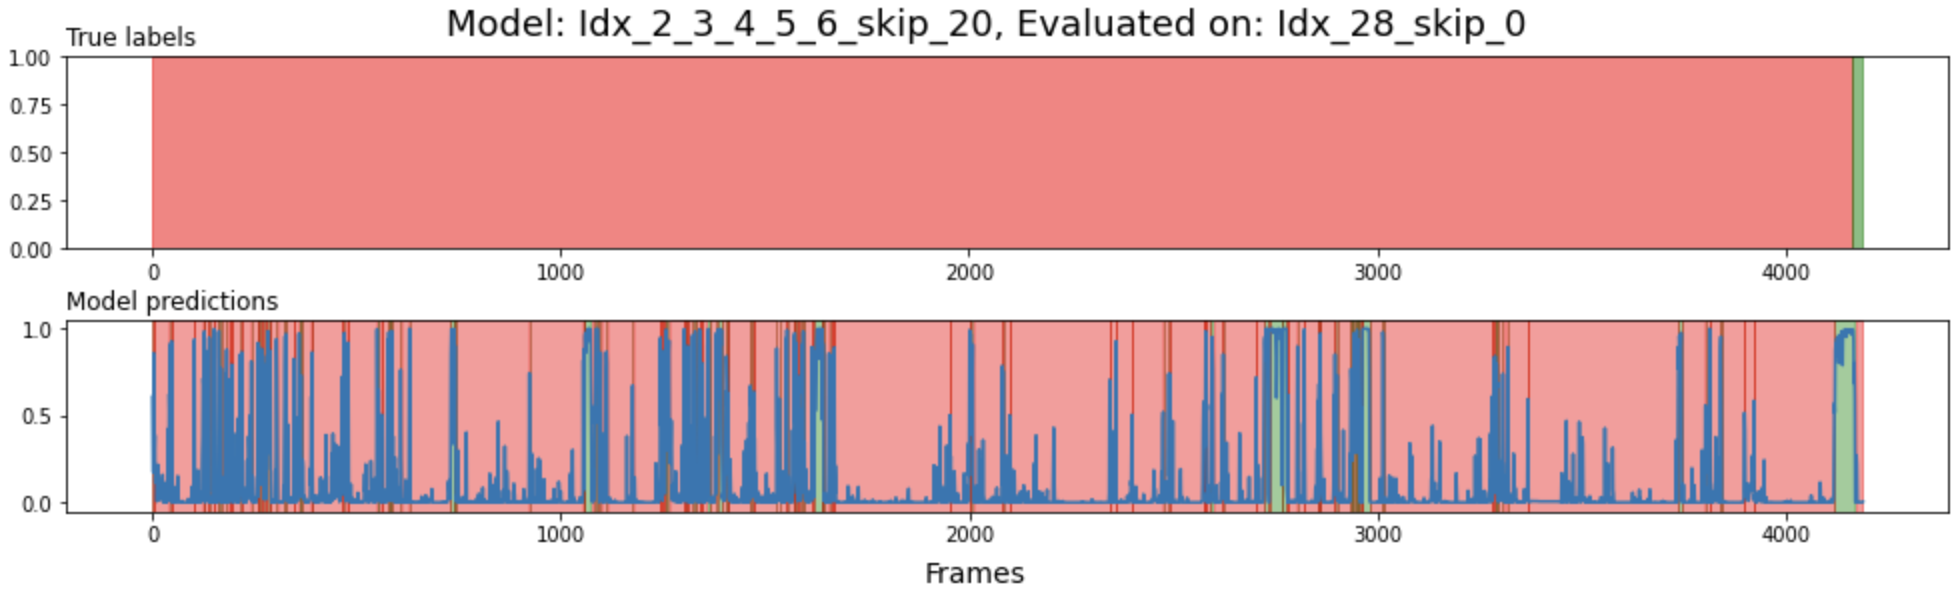
\includegraphics[width=\linewidth]{Materials/Results/SP/M4On28C}
	\end{subfigure}
	\\
	\begin{subfigure}{\linewidth}
		\centering
		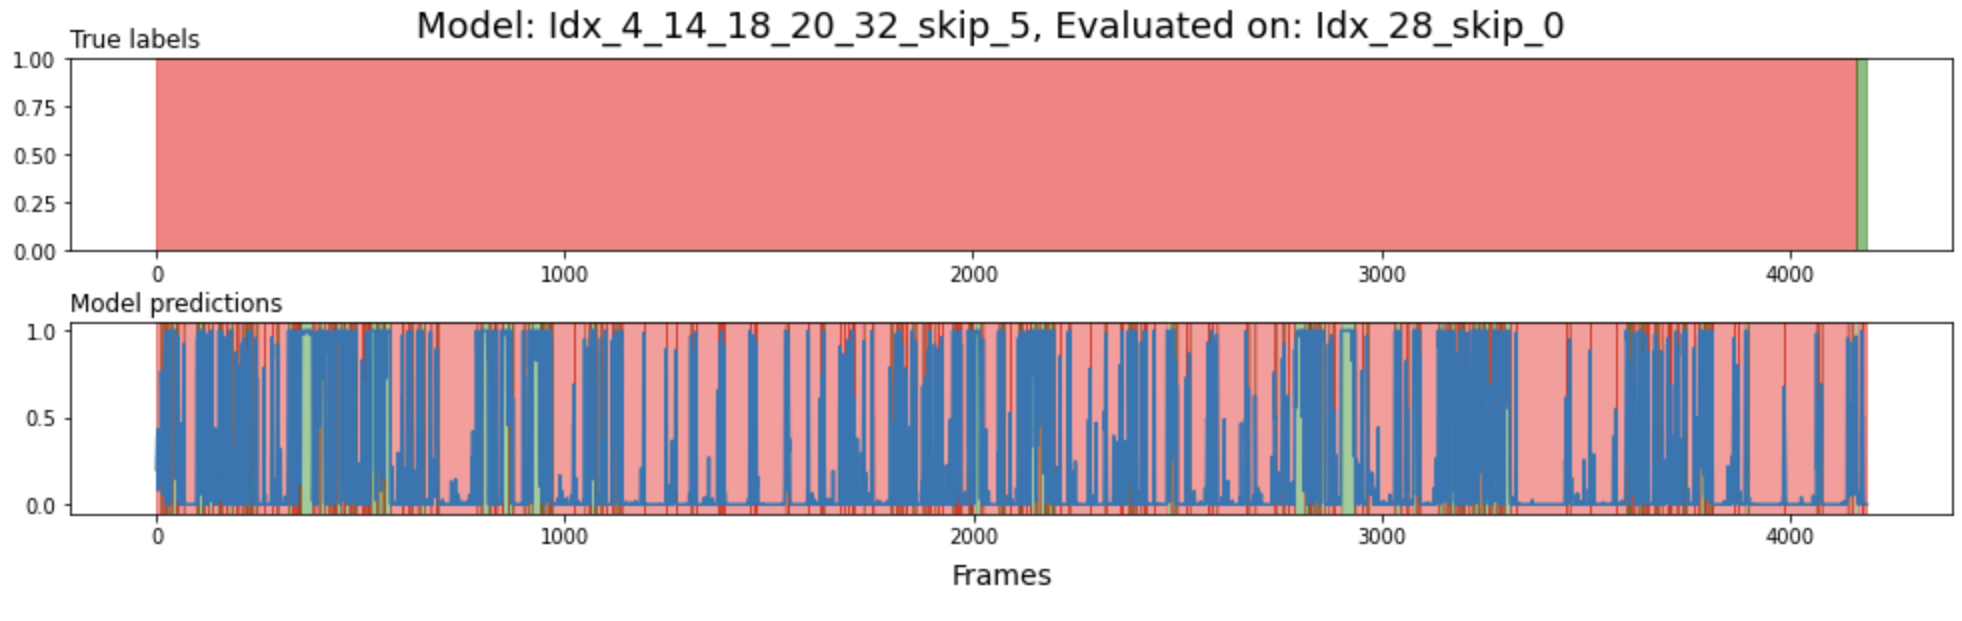
\includegraphics[width=\linewidth]{Materials/Results/SP/M6On28C}
	\end{subfigure}
	\caption{How the two selected models perform on test set \textit{Idx\_28\_skip\_0}.}
	\label{idx28}
\end{figure}

Based on these results model \textit{Idx\_2\_3\_4\_5\_6\_skip\_20} is considered to be the most accurate, and will be used moving forward towards predicting separation points and treatments.
\subsection{Separation point prediction}
Having decided on a model to move forward with, we can now evaluate how well the post-processing approaches performed by looking at their separation point predictions.

\begin{figure}[H]
	\centering
	\begin{subfigure}{\linewidth}
		\centering
		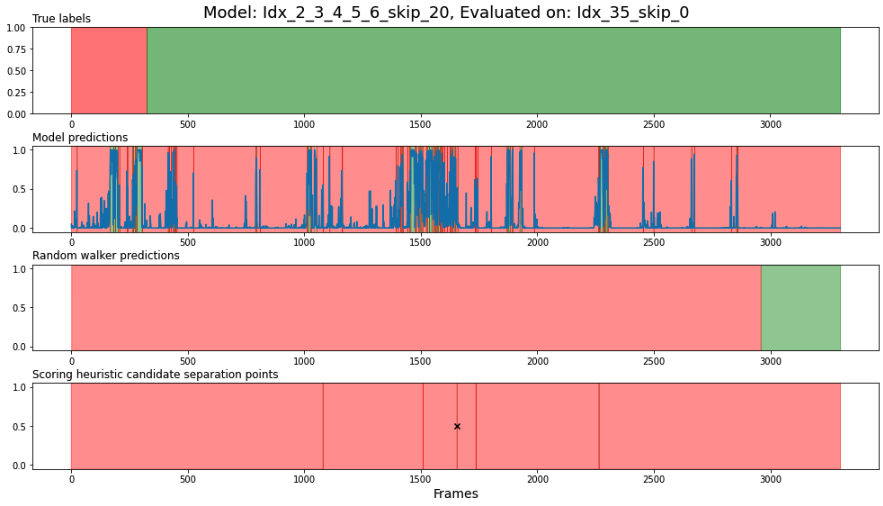
\includegraphics[width=\linewidth]{Materials/Results/SP/M4On35}
	\end{subfigure}
	\\
	\begin{subfigure}{\linewidth}
		\centering
		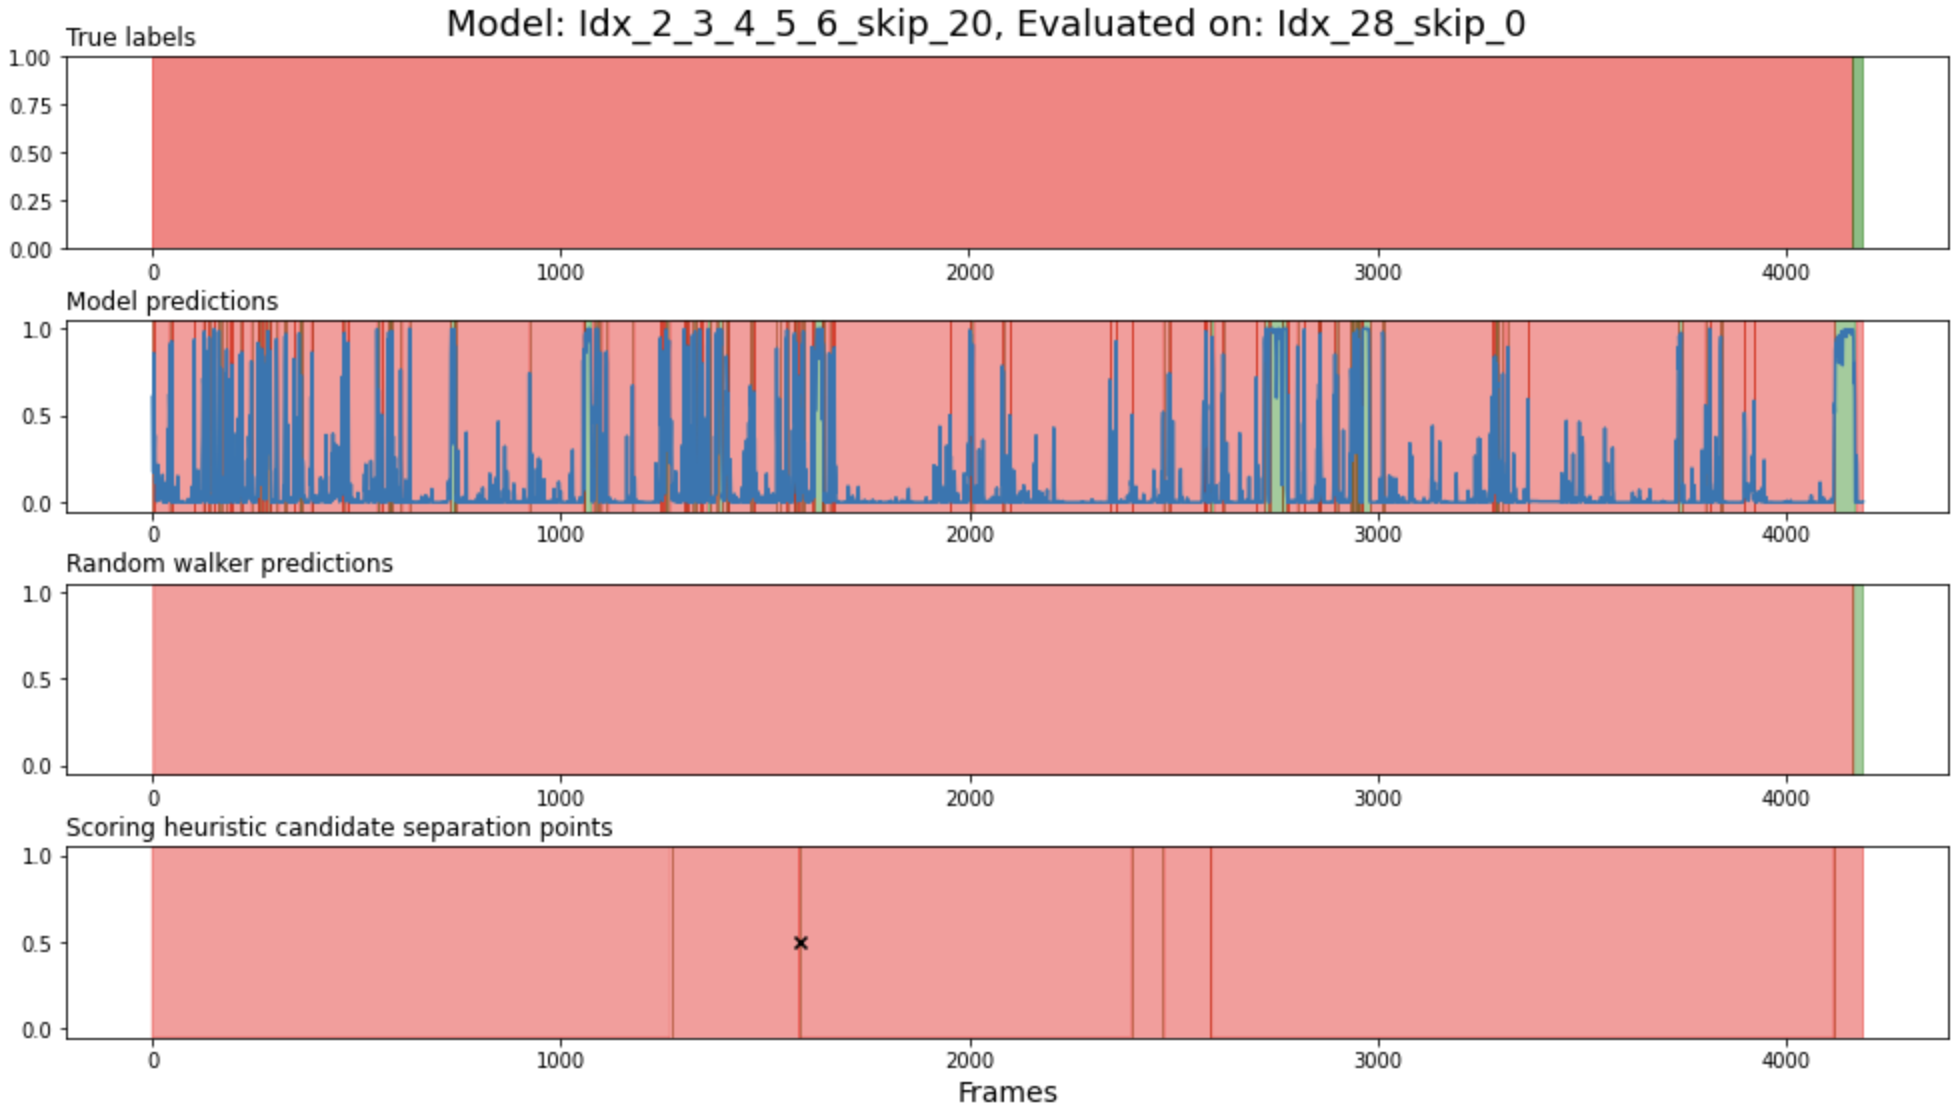
\includegraphics[width=\linewidth]{Materials/Results/SP/M4On28}
	\end{subfigure}
	\caption{Two separation point results.}
	\label{SPRes}
\end{figure}
In \autoref{SPRes} we see two evaluations, each consisting of four bars where the top bar is the true segmentation, the second is model prediction, third is the result of applying the Random Walker post-processing and the fourth is the result of applying the scoring heuristic. It should be noted the scoring heuristic predicts candidate points and one 'believed separation point' marked with an 'x'. This means, the marked points are 'transitions' which has a score less than $0.3$, and the 'x' marks the median of the lowest scoring 'transitions'. The scoring heuristic bar should thus not be read as a segmentation, but as several possible and one believed separation point.

Given the two examples in \autoref{SPRes} we see a tendency for the Random Walker to predict a 'high' separation point, whereas the scoring heuristic is rather insecure due to the insecure model predictions. These are general trends which also can be seen in \autoref{SPTable} where the results for all suitable videos has been reported. Videos 2 through 6 has not been reported as the model was trained on these.\\ 
In \autoref{SPTable} we see the true separation points (row 'True'), the predicted separation points for both post-processing approaches (row 'SH P' and 'RW P'), how far each prediction was from the true separation point measured in absolute number of frames (row 'SH \#' and 'RW \#'), and how far each prediction was measured in percentage of the total number of frames in the video (row 'SH \%' and 'RW \%').

\begin{table}[H]
	\hspace{-1.3cm}
	\begin{tabular}{|c|c|c|c|c|c|c|c|c|c|c|c|c|c|c|c|}
		\hline
		idx   & \multicolumn{1}{c|}{\cellcolor[HTML]{E8E8E8}1}                           & \multicolumn{1}{c|}{\cellcolor[HTML]{E8E8E8}7}                           & \multicolumn{1}{c|}{\cellcolor[HTML]{E8E8E8}8}                           & \multicolumn{1}{c|}{\cellcolor[HTML]{E8E8E8}9}                          & \multicolumn{1}{c|}{\cellcolor[HTML]{E8E8E8}10}                        & \multicolumn{1}{c|}{\cellcolor[HTML]{E8E8E8}11}                        & \multicolumn{1}{c|}{\cellcolor[HTML]{E8E8E8}12}                        & \multicolumn{1}{c|}{\cellcolor[HTML]{E8E8E8}13}                          & \multicolumn{1}{c|}{\cellcolor[HTML]{E8E8E8}14}                          & \multicolumn{1}{c|}{\cellcolor[HTML]{E8E8E8}15}                          & \multicolumn{1}{c|}{\cellcolor[HTML]{E8E8E8}16}                          & \multicolumn{1}{c|}{\cellcolor[HTML]{E8E8E8}17}                          & \multicolumn{1}{c|}{\cellcolor[HTML]{E8E8E8}18}                          & \multicolumn{1}{c|}{\cellcolor[HTML]{E8E8E8}19}                          & \multicolumn{1}{c|}{\cellcolor[HTML]{E8E8E8}20}                          \\ \hline
		True  & \multicolumn{1}{c|}{\cellcolor[HTML]{E8E8E8}{\color[HTML]{000000} 1086}} & \multicolumn{1}{c|}{\cellcolor[HTML]{E8E8E8}{\color[HTML]{000000} 3303}} & \multicolumn{1}{c|}{\cellcolor[HTML]{E8E8E8}{\color[HTML]{000000} 241}}  & \multicolumn{1}{c|}{\cellcolor[HTML]{E8E8E8}{\color[HTML]{000000} 0}}   & \multicolumn{1}{c|}{\cellcolor[HTML]{E8E8E8}{\color[HTML]{000000} 0}}  & \multicolumn{1}{c|}{\cellcolor[HTML]{E8E8E8}{\color[HTML]{000000} 0}}  & \multicolumn{1}{c|}{\cellcolor[HTML]{E8E8E8}{\color[HTML]{000000} 0}}  & \multicolumn{1}{c|}{\cellcolor[HTML]{E8E8E8}{\color[HTML]{000000} 0}}    & \multicolumn{1}{c|}{\cellcolor[HTML]{E8E8E8}{\color[HTML]{000000} 1575}} & \multicolumn{1}{c|}{\cellcolor[HTML]{E8E8E8}{\color[HTML]{000000} 3300}} & \multicolumn{1}{c|}{\cellcolor[HTML]{E8E8E8}{\color[HTML]{000000} 3299}} & \multicolumn{1}{c|}{\cellcolor[HTML]{E8E8E8}{\color[HTML]{000000} 3301}} & \multicolumn{1}{c|}{\cellcolor[HTML]{E8E8E8}{\color[HTML]{000000} 4164}} & \multicolumn{1}{c|}{\cellcolor[HTML]{E8E8E8}{\color[HTML]{000000} 76}}   & \multicolumn{1}{c|}{\cellcolor[HTML]{E8E8E8}{\color[HTML]{000000} 1026}} \\ \hline
		RW P  & \cellcolor[HTML]{ECF4FF}1459                                             & \cellcolor[HTML]{ECF4FF}3279                                             & \cellcolor[HTML]{ECF4FF}202                                              & \cellcolor[HTML]{ECF4FF}4979                                            & \cellcolor[HTML]{ECF4FF}4644                                           & \cellcolor[HTML]{ECF4FF}3300                                           & \cellcolor[HTML]{ECF4FF}3281                                           & \cellcolor[HTML]{ECF4FF}3291                                             & \cellcolor[HTML]{ECF4FF}3291                                             & \cellcolor[HTML]{ECF4FF}3272                                             & \cellcolor[HTML]{ECF4FF}3260                                             & \cellcolor[HTML]{ECF4FF}3255                                             & \cellcolor[HTML]{ECF4FF}4167                                             & \cellcolor[HTML]{ECF4FF}803                                              & \cellcolor[HTML]{ECF4FF}2739                                             \\ \hline
		SH P  & \cellcolor[HTML]{CBCEFB}43                                               & \cellcolor[HTML]{CBCEFB}2345                                             & \cellcolor[HTML]{CBCEFB}107                                              & \cellcolor[HTML]{CBCEFB}614                                             & \cellcolor[HTML]{CBCEFB}2076                                           & \cellcolor[HTML]{CBCEFB}2895                                           & \cellcolor[HTML]{CBCEFB}1354                                           & \cellcolor[HTML]{CBCEFB}3179                                             & \cellcolor[HTML]{CBCEFB}3179                                             & \cellcolor[HTML]{CBCEFB}887                                              & \cellcolor[HTML]{CBCEFB}572                                              & \cellcolor[HTML]{CBCEFB}1400                                             & \cellcolor[HTML]{CBCEFB}4153                                             & \cellcolor[HTML]{CBCEFB}374                                              & \cellcolor[HTML]{CBCEFB}444                                              \\ \hline
		RW \# & \cellcolor[HTML]{ECF4FF}373                                              & \cellcolor[HTML]{ECF4FF}24                                               & \cellcolor[HTML]{ECF4FF}39                                               & \cellcolor[HTML]{ECF4FF}4979                                            & \cellcolor[HTML]{ECF4FF}4644                                           & \cellcolor[HTML]{ECF4FF}3300                                           & \cellcolor[HTML]{ECF4FF}3281                                           & \cellcolor[HTML]{ECF4FF}3291                                             & \cellcolor[HTML]{ECF4FF}1716                                             & \cellcolor[HTML]{ECF4FF}28                                               & \cellcolor[HTML]{ECF4FF}39                                               & \cellcolor[HTML]{ECF4FF}46                                               & \cellcolor[HTML]{ECF4FF}3                                                & \cellcolor[HTML]{ECF4FF}727                                              & \cellcolor[HTML]{ECF4FF}1713                                             \\ \hline
		SH \# & \cellcolor[HTML]{CBCEFB}1043                                             & \cellcolor[HTML]{CBCEFB}958                                              & \cellcolor[HTML]{CBCEFB}134                                              & \cellcolor[HTML]{CBCEFB}614                                             & \cellcolor[HTML]{CBCEFB}2076                                           & \cellcolor[HTML]{CBCEFB}2895                                           & \cellcolor[HTML]{CBCEFB}1354                                           & \cellcolor[HTML]{CBCEFB}3179                                             & \cellcolor[HTML]{CBCEFB}1604                                             & \cellcolor[HTML]{CBCEFB}2413                                             & \cellcolor[HTML]{CBCEFB}2727                                             & \cellcolor[HTML]{CBCEFB}1901                                             & \cellcolor[HTML]{CBCEFB}11                                               & \cellcolor[HTML]{CBCEFB}298                                              & \cellcolor[HTML]{CBCEFB}582                                              \\ \hline
		RW \% & \cellcolor[HTML]{ECF4FF}0.25                                             & \cellcolor[HTML]{ECF4FF}0.01                                             & \cellcolor[HTML]{ECF4FF}0.16                                             & \cellcolor[HTML]{ECF4FF}1.00                                            & \cellcolor[HTML]{ECF4FF}0.93                                           & \cellcolor[HTML]{ECF4FF}0.66                                           & \cellcolor[HTML]{ECF4FF}0.99                                           & \cellcolor[HTML]{ECF4FF}1.00                                             & \cellcolor[HTML]{ECF4FF}0.52                                             & \cellcolor[HTML]{ECF4FF}0.01                                             & \cellcolor[HTML]{ECF4FF}0.01                                             & \cellcolor[HTML]{ECF4FF}0.01                                             & \cellcolor[HTML]{ECF4FF}0.00                                             & \cellcolor[HTML]{ECF4FF}0.87                                             & \cellcolor[HTML]{ECF4FF}0.52                                             \\ \hline
		SH \% & \cellcolor[HTML]{CBCEFB}0.70                                             & \cellcolor[HTML]{CBCEFB}0.29                                             & \cellcolor[HTML]{CBCEFB}0.56                                             & \cellcolor[HTML]{CBCEFB}0.12                                            & \cellcolor[HTML]{CBCEFB}0.42                                           & \cellcolor[HTML]{CBCEFB}0.58                                           & \cellcolor[HTML]{CBCEFB}0.41                                           & \cellcolor[HTML]{CBCEFB}0.96                                             & \cellcolor[HTML]{CBCEFB}0.49                                             & \cellcolor[HTML]{CBCEFB}0.73                                             & \cellcolor[HTML]{CBCEFB}0.83                                             & \cellcolor[HTML]{CBCEFB}0.58                                             & \cellcolor[HTML]{CBCEFB}0.00                                             & \cellcolor[HTML]{CBCEFB}0.36                                             & \cellcolor[HTML]{CBCEFB}0.18                                             \\ \hline\hline
		idx   & \multicolumn{1}{c|}{\cellcolor[HTML]{E8E8E8}{\color[HTML]{000000} 21}}   & \multicolumn{1}{c|}{\cellcolor[HTML]{E8E8E8}{\color[HTML]{000000} 22}}   & \multicolumn{1}{c|}{\cellcolor[HTML]{E8E8E8}{\color[HTML]{000000} 23}}   & \multicolumn{1}{c|}{\cellcolor[HTML]{E8E8E8}{\color[HTML]{000000} 24}}  & \multicolumn{1}{c|}{\cellcolor[HTML]{E8E8E8}{\color[HTML]{000000} 25}} & \multicolumn{1}{c|}{\cellcolor[HTML]{E8E8E8}{\color[HTML]{000000} 26}} & \multicolumn{1}{c|}{\cellcolor[HTML]{E8E8E8}{\color[HTML]{000000} 27}} & \multicolumn{1}{c|}{\cellcolor[HTML]{E8E8E8}{\color[HTML]{000000} 28}}   & \multicolumn{1}{c|}{\cellcolor[HTML]{E8E8E8}{\color[HTML]{000000} 29}}   & \multicolumn{1}{c|}{\cellcolor[HTML]{E8E8E8}{\color[HTML]{000000} 30}}   & \multicolumn{1}{c|}{\cellcolor[HTML]{E8E8E8}{\color[HTML]{000000} 31}}   & \multicolumn{1}{c|}{\cellcolor[HTML]{E8E8E8}{\color[HTML]{000000} 32}}   & \multicolumn{1}{c|}{\cellcolor[HTML]{E8E8E8}{\color[HTML]{000000} 33}}   & \multicolumn{1}{c|}{\cellcolor[HTML]{E8E8E8}{\color[HTML]{000000} 34}}   & \multicolumn{1}{c|}{\cellcolor[HTML]{E8E8E8}{\color[HTML]{000000} 35}}   \\ \hline
		True  & \multicolumn{1}{c|}{\cellcolor[HTML]{E8E8E8}{\color[HTML]{000000} 3295}} & \multicolumn{1}{c|}{\cellcolor[HTML]{E8E8E8}{\color[HTML]{000000} 3299}} & \multicolumn{1}{c|}{\cellcolor[HTML]{E8E8E8}{\color[HTML]{000000} 3119}} & \multicolumn{1}{c|}{\cellcolor[HTML]{E8E8E8}{\color[HTML]{000000} 402}} & \multicolumn{1}{c|}{\cellcolor[HTML]{E8E8E8}{\color[HTML]{000000} 0}}  & \multicolumn{1}{c|}{\cellcolor[HTML]{E8E8E8}{\color[HTML]{000000} 0}}  & \multicolumn{1}{c|}{\cellcolor[HTML]{E8E8E8}{\color[HTML]{000000} 0}}  & \multicolumn{1}{c|}{\cellcolor[HTML]{E8E8E8}{\color[HTML]{000000} 4164}} & \multicolumn{1}{c|}{\cellcolor[HTML]{E8E8E8}{\color[HTML]{000000} 0}}    & \multicolumn{1}{c|}{\cellcolor[HTML]{E8E8E8}{\color[HTML]{000000} 0}}    & \multicolumn{1}{c|}{\cellcolor[HTML]{E8E8E8}{\color[HTML]{000000} 0}}    & \multicolumn{1}{c|}{\cellcolor[HTML]{E8E8E8}{\color[HTML]{000000} 0}}    & \multicolumn{1}{c|}{\cellcolor[HTML]{E8E8E8}{\color[HTML]{000000} 3299}} & \multicolumn{1}{c|}{\cellcolor[HTML]{E8E8E8}{\color[HTML]{000000} 3302}} & \multicolumn{1}{c|}{\cellcolor[HTML]{E8E8E8}{\color[HTML]{000000} 325}}  \\ \hline
		RW P  & \cellcolor[HTML]{ECF4FF}2446                                             & \cellcolor[HTML]{ECF4FF}3261                                             & \cellcolor[HTML]{ECF4FF}3270                                             & \cellcolor[HTML]{ECF4FF}1880                                            & \cellcolor[HTML]{ECF4FF}4978                                           & \cellcolor[HTML]{ECF4FF}4779                                           & \cellcolor[HTML]{ECF4FF}4674                                           & \cellcolor[HTML]{ECF4FF}4167                                             & \cellcolor[HTML]{ECF4FF}49                                               & \cellcolor[HTML]{ECF4FF}3259                                             & \cellcolor[HTML]{ECF4FF}3293                                             & \cellcolor[HTML]{ECF4FF}3261                                             & \cellcolor[HTML]{ECF4FF}3296                                             & \cellcolor[HTML]{ECF4FF}3295                                             & \cellcolor[HTML]{ECF4FF}2958                                             \\ \hline
		SH P  & \cellcolor[HTML]{CBCEFB}2441                                             & \cellcolor[HTML]{CBCEFB}543                                              & \cellcolor[HTML]{CBCEFB}1221                                             & \cellcolor[HTML]{CBCEFB}1428                                            & \cellcolor[HTML]{CBCEFB}1672                                           & \cellcolor[HTML]{CBCEFB}2113                                           & \cellcolor[HTML]{CBCEFB}4672                                           & \cellcolor[HTML]{CBCEFB}4153                                             & \cellcolor[HTML]{CBCEFB}53                                               & \cellcolor[HTML]{CBCEFB}2202                                             & \cellcolor[HTML]{CBCEFB}2586                                             & \cellcolor[HTML]{CBCEFB}3052                                             & \cellcolor[HTML]{CBCEFB}2562                                             & \cellcolor[HTML]{CBCEFB}1614                                             & \cellcolor[HTML]{CBCEFB}1653                                             \\ \hline
		RW \# & \cellcolor[HTML]{ECF4FF}849                                              & \cellcolor[HTML]{ECF4FF}38                                               & \cellcolor[HTML]{ECF4FF}151                                              & \cellcolor[HTML]{ECF4FF}1478                                            & \cellcolor[HTML]{ECF4FF}4978                                           & \cellcolor[HTML]{ECF4FF}4779                                           & \cellcolor[HTML]{ECF4FF}4674                                           & \cellcolor[HTML]{ECF4FF}3                                                & \cellcolor[HTML]{ECF4FF}49                                               & \cellcolor[HTML]{ECF4FF}3259                                             & \cellcolor[HTML]{ECF4FF}3293                                             & \cellcolor[HTML]{ECF4FF}3261                                             & \cellcolor[HTML]{ECF4FF}3                                                & \cellcolor[HTML]{ECF4FF}7                                                & \cellcolor[HTML]{ECF4FF}2633                                             \\ \hline
		SH \# & \cellcolor[HTML]{CBCEFB}854                                              & \cellcolor[HTML]{CBCEFB}2756                                             & \cellcolor[HTML]{CBCEFB}1898                                             & \cellcolor[HTML]{CBCEFB}1026                                            & \cellcolor[HTML]{CBCEFB}1672                                           & \cellcolor[HTML]{CBCEFB}2113                                           & \cellcolor[HTML]{CBCEFB}4672                                           & \cellcolor[HTML]{CBCEFB}11                                               & \cellcolor[HTML]{CBCEFB}53                                               & \cellcolor[HTML]{CBCEFB}2202                                             & \cellcolor[HTML]{CBCEFB}2586                                             & \cellcolor[HTML]{CBCEFB}3052                                             & \cellcolor[HTML]{CBCEFB}737                                              & \cellcolor[HTML]{CBCEFB}1688                                             & \cellcolor[HTML]{CBCEFB}1328                                             \\ \hline
		RW \% & \cellcolor[HTML]{ECF4FF}0.26                                             & \cellcolor[HTML]{ECF4FF}0.01                                             & \cellcolor[HTML]{ECF4FF}0.05                                             & \cellcolor[HTML]{ECF4FF}0.68                                            & \cellcolor[HTML]{ECF4FF}1.00                                           & \cellcolor[HTML]{ECF4FF}0.96                                           & \cellcolor[HTML]{ECF4FF}1.00                                           & \cellcolor[HTML]{ECF4FF}0.00                                             & \cellcolor[HTML]{ECF4FF}0.88                                             & \cellcolor[HTML]{ECF4FF}0.99                                             & \cellcolor[HTML]{ECF4FF}1.00                                             & \cellcolor[HTML]{ECF4FF}0.99                                             & \cellcolor[HTML]{ECF4FF}0.00                                             & \cellcolor[HTML]{ECF4FF}0.00                                             & \cellcolor[HTML]{ECF4FF}0.80                                             \\ \hline
		SH \% & \cellcolor[HTML]{CBCEFB}0.26                                             & \cellcolor[HTML]{CBCEFB}0.84                                             & \cellcolor[HTML]{CBCEFB}0.58                                             & \cellcolor[HTML]{CBCEFB}0.47                                            & \cellcolor[HTML]{CBCEFB}0.34                                           & \cellcolor[HTML]{CBCEFB}0.42                                           & \cellcolor[HTML]{CBCEFB}1.00                                           & \cellcolor[HTML]{CBCEFB}0.00                                             & \cellcolor[HTML]{CBCEFB}0.95                                             & \cellcolor[HTML]{CBCEFB}0.67                                             & \cellcolor[HTML]{CBCEFB}0.78                                             & \cellcolor[HTML]{CBCEFB}0.93                                             & \cellcolor[HTML]{CBCEFB}0.22                                             & \cellcolor[HTML]{CBCEFB}0.51                                             & \cellcolor[HTML]{CBCEFB}0.40                                             \\ \hline
	\end{tabular}
	\caption{Separation point predictions for all suitable videos. Each video has been enumerated and given and index to be identified with. The 'True' row depicts the true separation point. 'RW P' is the separation point predicted by the Random Walker. 'SH P' is the predicted separation point for the scoring heuristic (the believed point). 'RW \#' is the absolute number of frames to the true separation point from the Random Walker prediction. 'SH \#' is the absolute number of frames to the true separation point from the scoring heuristic prediction. 'RW \%' is the number of frames from the Random Walker prediction to the true separation point measured as a percentage of the total number of frames in the video. 'SH \%' is the number of frames from the Scoring heuristic prediction to the true separation point measured as a percentage of the total number of frames in the video.}
	\label{SPTable}
\end{table}
Taking a closer look at the results in \autoref{SPTable}, we see the average distance in frames from predictions to true separation points for the Random Walker approach is $1788.6$ frames, while for the scoring heuristic this is $1614.57$ frames. However, if we compute the distances in percentages of the total number of frames Random Walker comes out with an average of $51.85\%$ and the scoring heuristic with $51.87\%$.\\
Taking a look at the distance between the predictions and true separation points in terms of frames for the Random Walker approach (row 'RW \#') we see a quite large variance, as some of the videos with a lot of inflamed frames are predicted very accurately, while most of the videos with a lot of healthy frames are predicted very poorly. In general we see the Random Walker approach being very conservative, and predicting 'high' separation points.\\
Looking at the distance between the predictions and true separation points for the scoring heuristic (row 'SH \#'), we see a lower variance as the scoring heuristic is more willing to predict lower separation points on the videos with many healthy frames, however, it is not as accurate on the videos with a lot of inflamed frames as the Random Walker approach is.
\subsection{Treatment prediction}
Because only 30 data vectors were available and model \textit{Idx\_2\_3\_4\_5\_6\_skip\_20} was trained on five datasets, only 25 data vectors were available for predicting treatments. Two slightly different approaches of training was thus attempted. First, training was conducted by a 'leave-one-out' strategy where a 1D ResNet was trained on 24 data vectors and tested on the last one, while rotating which data vector was left out, and training a new model for each rotation. In the second approach, the true segmentations was included in training which would give 48 training vectors. The same leave-one-out strategy was deployed, but only the predicted segmentation would be used for testing. Each model was trained for 120 epochs, using cross entropy as loss function and Adam for optimization with a learning rate of $10^{-4}$ and with a weight decay of $0.07$. 

\begin{table}[H]
	\hspace{-2.7cm}
	\begin{tabular}{|c|c|c|c|c|c|c|c|c|c|c|c|c|c|c|c|c|c|c|c|c|c|c|c|c|c|}
		\hline
		Idx&1
		&7
		&8
		&14
		&15
		&16
		&17
		&18
		&19
		&20
		&21
		&22
		&23
		&24
		&25
		&26
		&27
		&28
		&29
		&30
		&31
		&32
		&33
		&34
		&35\\\hline\hline
		Predictions&2
		&0
		&0
		&2
		&2
		&0
		&2
		&2
		&2
		&2
		&2
		&2
		&2
		&2
		&2
		&2
		&2
		&2
		&0
		&0
		&2
		&2
		&0
		&2
		&2\\\hline
		True&1
		&3
		&3
		&4
		&2
		&2
		&2
		&1
		&1
		&2
		&2
		&2
		&2
		&1
		&0
		&0
		&0
		&1
		&0
		&0
		&0
		&0
		&2
		&2
		&2\\\hline
	\end{tabular}
	\caption{Training a model only on the predicted segmentations, we find the following treatment predictions and true treatments shown for each video. The treatment classes are: 0 being 'healthy', 1 being 'local 5-ASA', 2 being 'Oral steroid', 3 being 'IV steroid' and 4 being 'oral 5-ASA'.}
	\label{treatmentTable}
\end{table}


\begin{figure}[H]
	\centering
	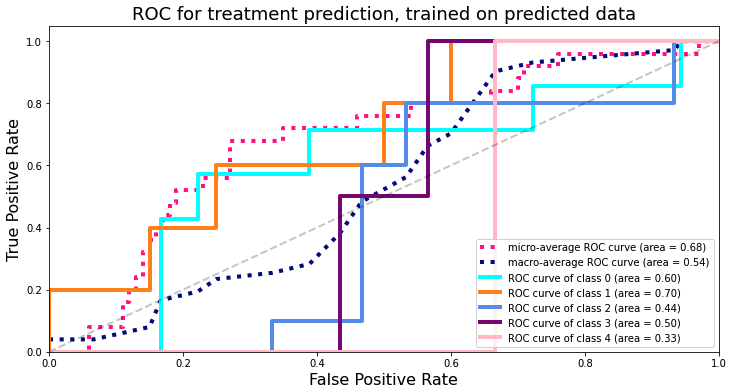
\includegraphics[width=0.85\linewidth]{Materials/Results/Treatment/RocPreds}
	\caption{ROC curves and area under the curve for the five binary 'one-vs-rest' classifiers along with micro- and macro-averages. Training was performed only on predicted segmentations.}
	\label{rocpreds}
\end{figure}
In \autoref{treatmentTable} we see the predicted treatments along the true prescribed treatment, when we train only on predicted segmentations from model \textit{Idx\_2\_3\_4\_5\_6\_skip\_20}. Computing the accuracy of this approach we get $40\%$. However, we note the model only have predicted class 2 and class 0, and there is a heavy class imbalance in the data, with only two examples of class 3 and one example of class 4.\\
It can be hard to assert the quality of a multi class classifier based on accuracy, and thus five binary 'one-vs-rest' classifiers was trained with the same parameters as the original multi class classifier. These binary models was then used to draw ROC curves for which the area under the curves could be computed. The results can be seen in \autoref{rocpreds}.

In \autoref{treatmentTableWithTrue} we see the treatment predictions and true prescribed treatment for each video for a model trained on the predicted segmentations from model \textit{Idx\_2\_3\_4\_5\_6\_skip\_20} and the true segmentations. This model was trained with the same parameters as the previous treatment prediction model. Computing the accuracy we get $48\%$, but we again note only class 0 and class 2 is predicted.
\begin{table}[H]
	\hspace{-2.7cm}
	\begin{tabular}{|c|c|c|c|c|c|c|c|c|c|c|c|c|c|c|c|c|c|c|c|c|c|c|c|c|c|}
		\hline
		Idx&1
		&7
		&8
		&14
		&15
		&16
		&17
		&18
		&19
		&20
		&21
		&22
		&23
		&24
		&25
		&26
		&27
		&28
		&29
		&30
		&31
		&32
		&33
		&34
		&35\\\hline\hline
		Predictions&2
		&0
		&0
		&2
		&2
		&2
		&2
		&2
		&2
		&2
		&2
		&2
		&2
		&2
		&2
		&2
		&2
		&2
		&0
		&0
		&2
		&0
		&0
		&2
		&2\\\hline
		True&1
		&3
		&3
		&4
		&2
		&2
		&2
		&1
		&1
		&2
		&2
		&2
		&2
		&1
		&0
		&0
		&0
		&1
		&0
		&0
		&0
		&0
		&2
		&2
		&2\\\hline
	\end{tabular}
	\caption{Training a model on both the predicted segmentations and true segmentations, we find the following treatment predictions and true treatments shown for each video. The treatment classes are: 0 being 'healthy', 1 being 'local 5-ASA', 2 being 'Oral steroid', 3 being 'IV steroid' and 4 being 'oral 5-ASA'.}
	\label{treatmentTableWithTrue}
\end{table}

In \autoref{rocpredsandtrue} ROC curves are drawn for each of the five binary 'one-vs-rest' classifiers, trained with the same parameters as the original multi class classifier and trained on both predicted and true segmentations.

\begin{figure}[H]
	\centering
	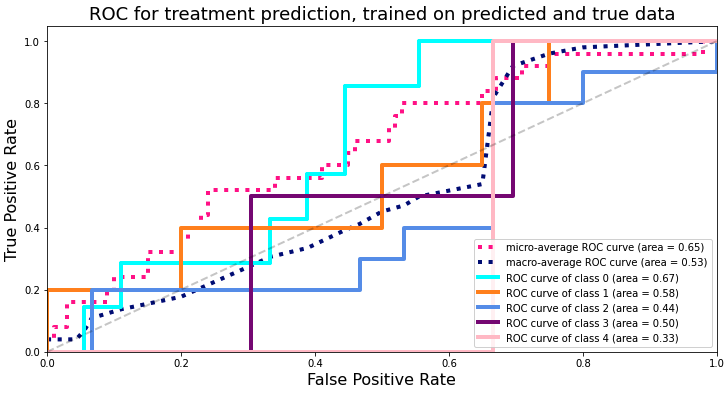
\includegraphics[width=0.85\linewidth]{Materials/Results/Treatment/RocPredsAndTrue}
	\caption{ROC curves and area under the curve for the five binary 'one-vs-rest' classifiers along with micro- and macro-averages. Training was performed on both predicted and true segmentations.}
	\label{rocpredsandtrue}
\end{figure}
\subsection{U-Net for video segmentation}
In an attempt to make the predicted video segmentations from the 2D ResNet model more structured, a 1D U-Net was trained on the predictions of model \textit{Idx\_2\_3\_4\_5\_6\_skip\_20}. Training was conducted in a 'leave-one-out' fashion on the 25 predicted segmentations suitable for treatment predictions. The model was trained for 100 epochs with a learning rate of $3\cdot 10^{-6}$, binary cross entropy as loss function, Adam for optimization and $0.25$ weight decay.\\
The true segmentations was used as target, and was 'artificially' constructed by concatenating a vector of zeros equal in length to the number of frames up to the true separation point, and a vector of ones equal in length to the remaining frames of the video, such that we get one continuous block of inflammation predictions followed by one continuous block of healthy predictions which correspond to how the doctor annotated the video.\\
In the following, four predictions will be reported to show the effect of the trained U-Net model. In each illustration the true segmentation will be shown as the top bar, the 2D ResNet prediction will be shown as the second bar, and the 1D U-Net prediction and its confidence in a healthy prediction will be shown as the third bar.

\begin{figure}[H]
	\centering
	\begin{subfigure}{\linewidth}
		\centering
		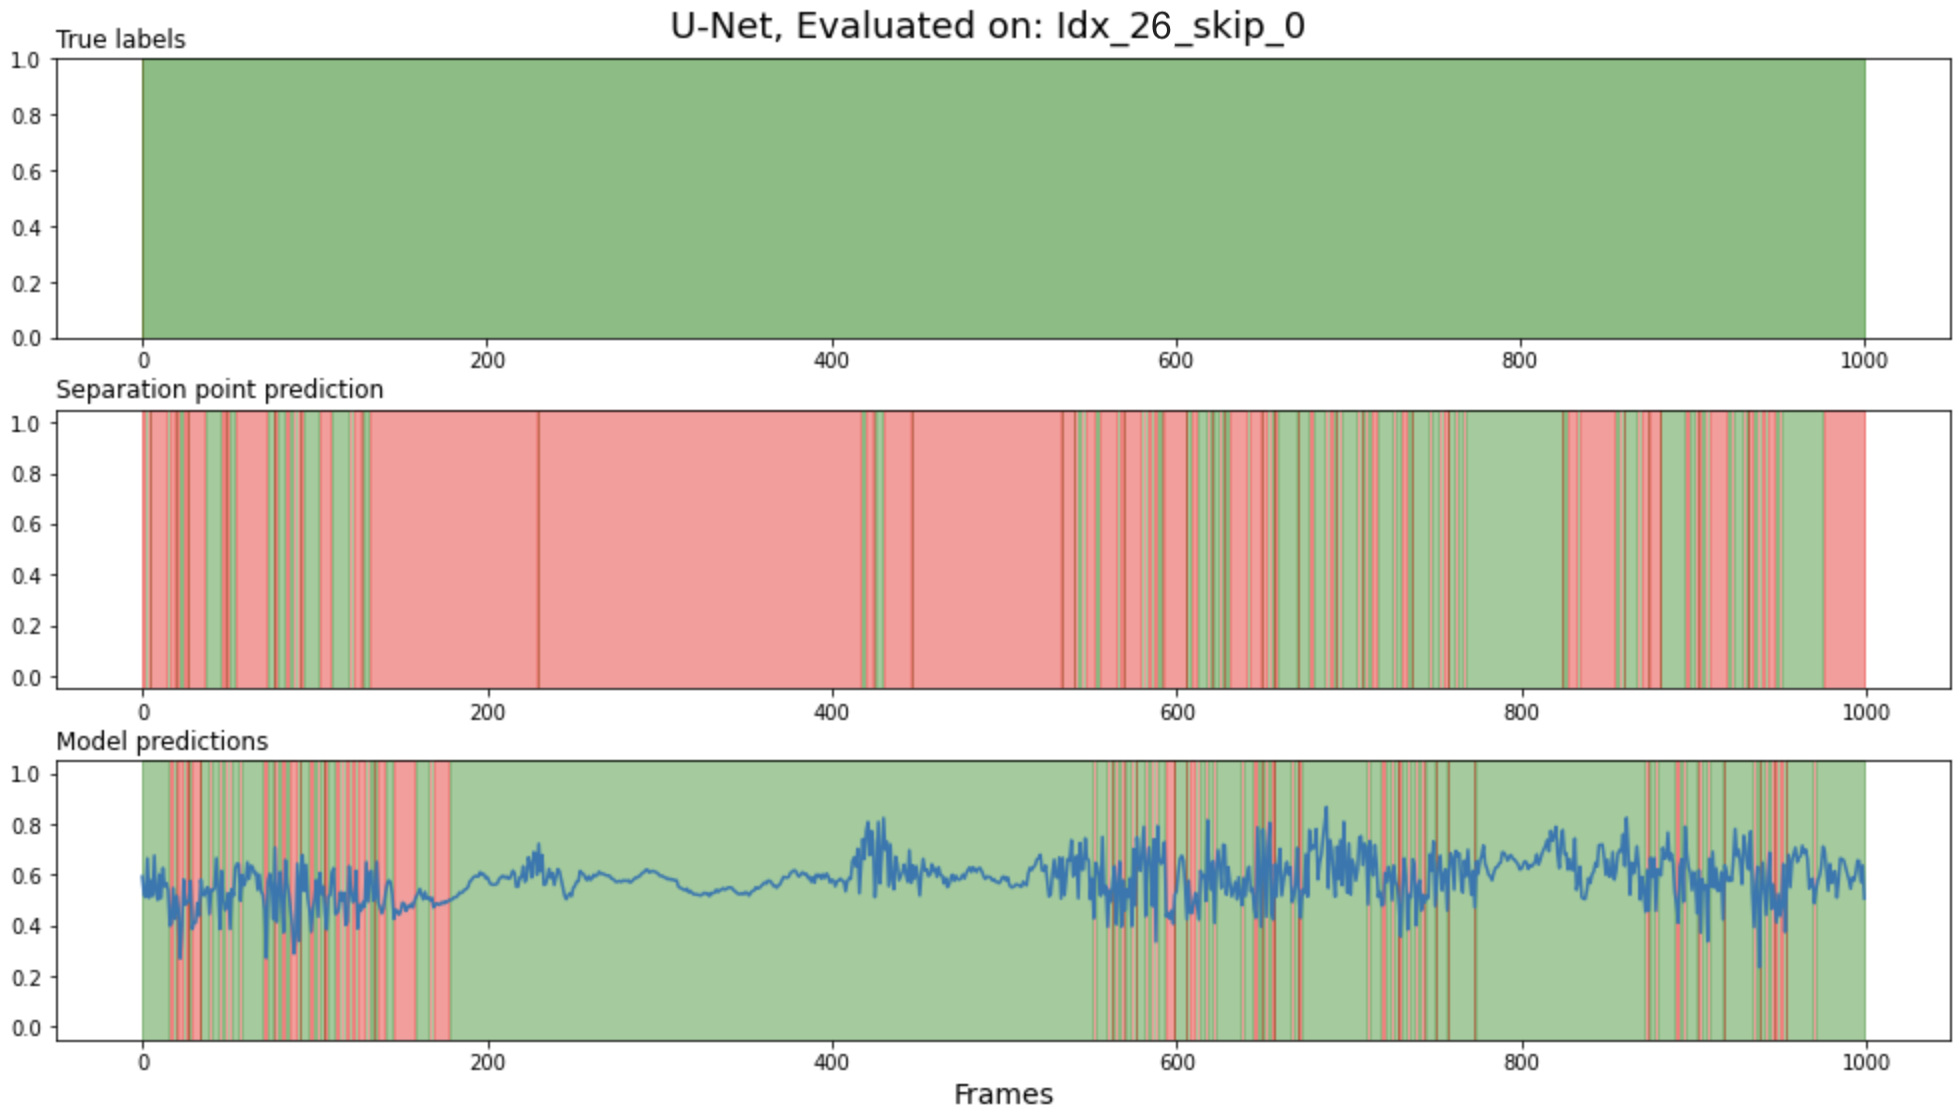
\includegraphics[width=\linewidth]{Materials/Results/UNet/unet1}
	\end{subfigure}
	\\
	\begin{subfigure}{\linewidth}
		\centering
		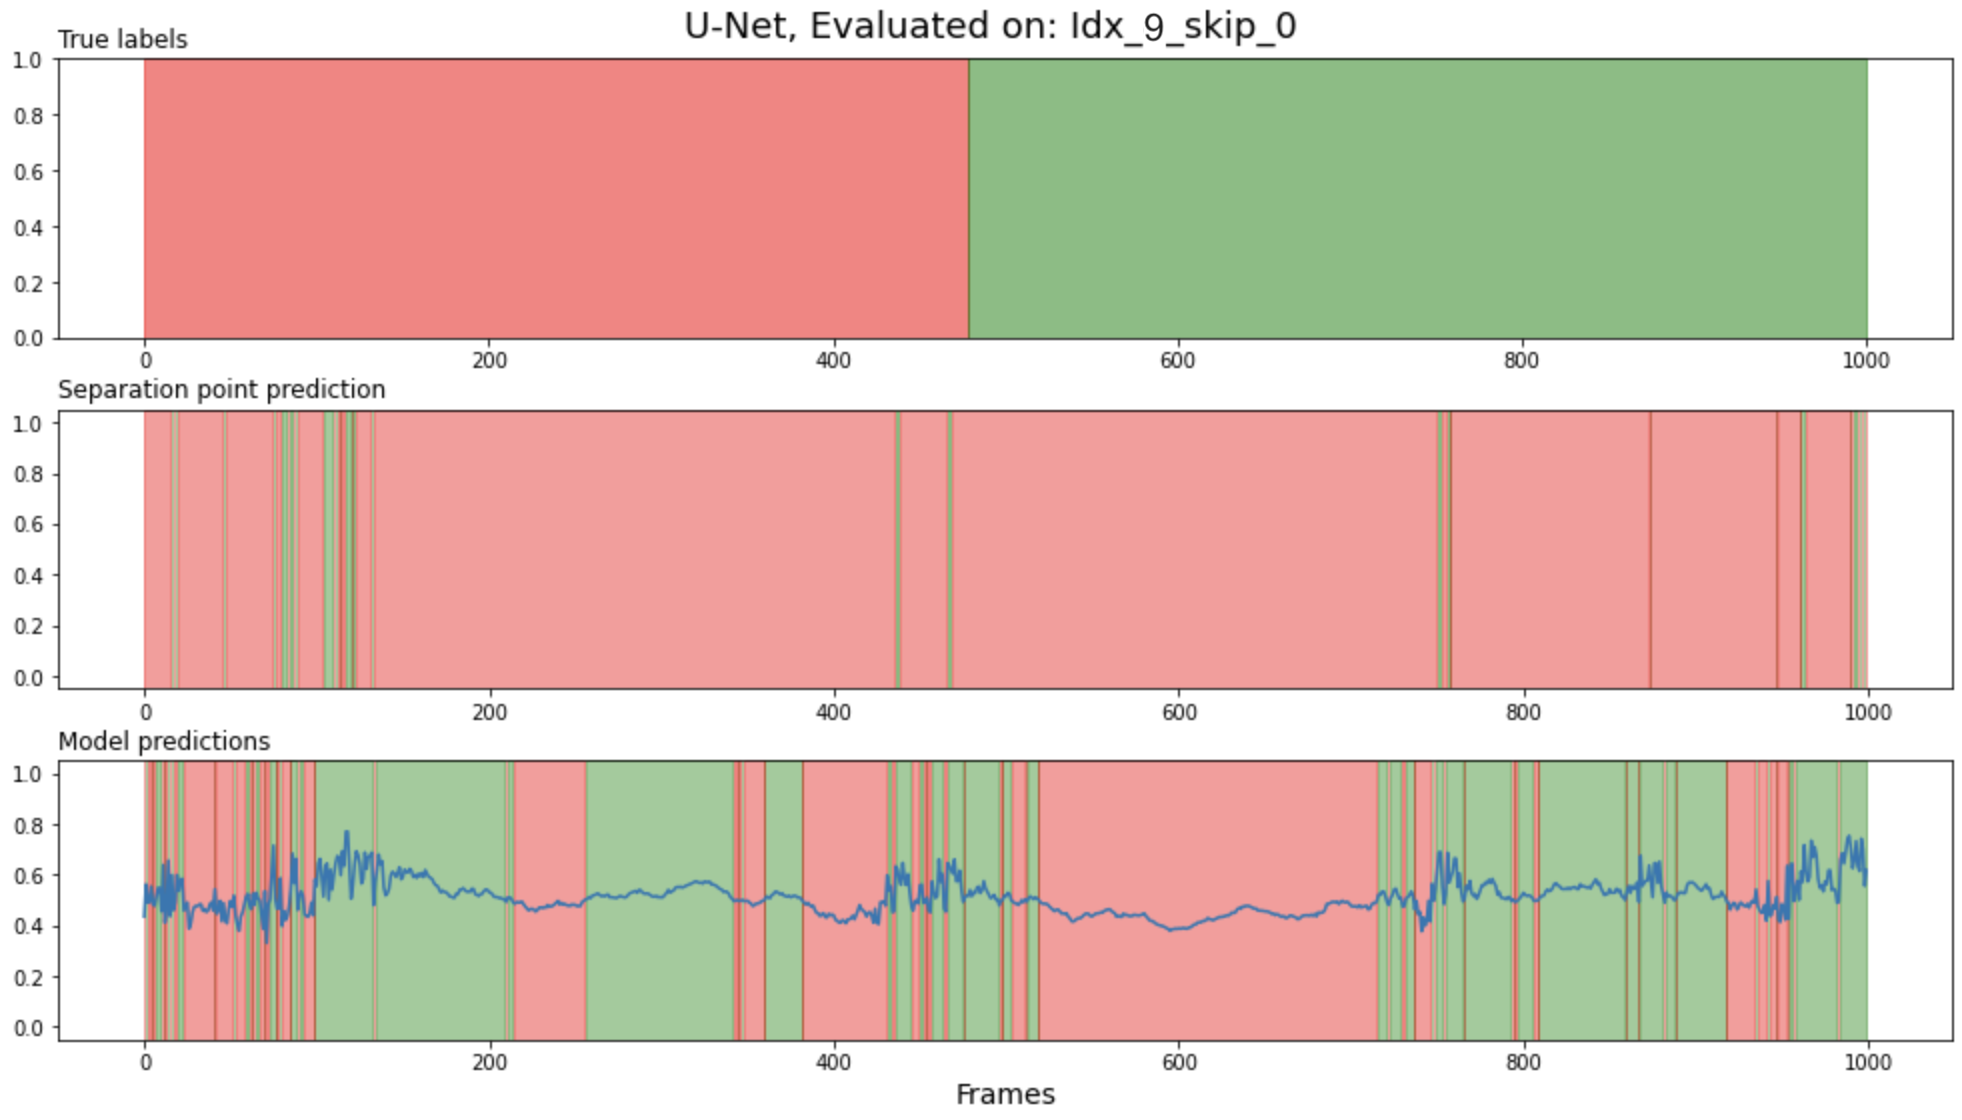
\includegraphics[width=\linewidth]{Materials/Results/UNet/unet2}
	\end{subfigure}
	\caption{Results of 1D U-Net model.}
	\label{unetres1}
\end{figure}

Taking a look at the first result presented in \autoref{unetres1}, we see the true segmentation is all healthy, but the ResNet prediction has a lot of inflammation predictions. Although the U-Net model is not confident in its predictions, it is certain in the sense it does not have very big oscillations. We also see the U-Net predictions have overturned a lot of the inflammation predictions, and made the prediction a lot more representative to the true segmentation.\\
Looking at the second prediction in \autoref{unetres1}, we see the true segmentation being almost half inflammation and half healthy. The ResNet predictions are however almost exclusively inflammation. Again we see the U-Net predictions being very steady and overturning a lot of the inflammation predictions, however this time also making correctly predicted inflamed frames healthy.

\begin{figure}[H]
	\centering
	\begin{subfigure}{\linewidth}
		\centering
		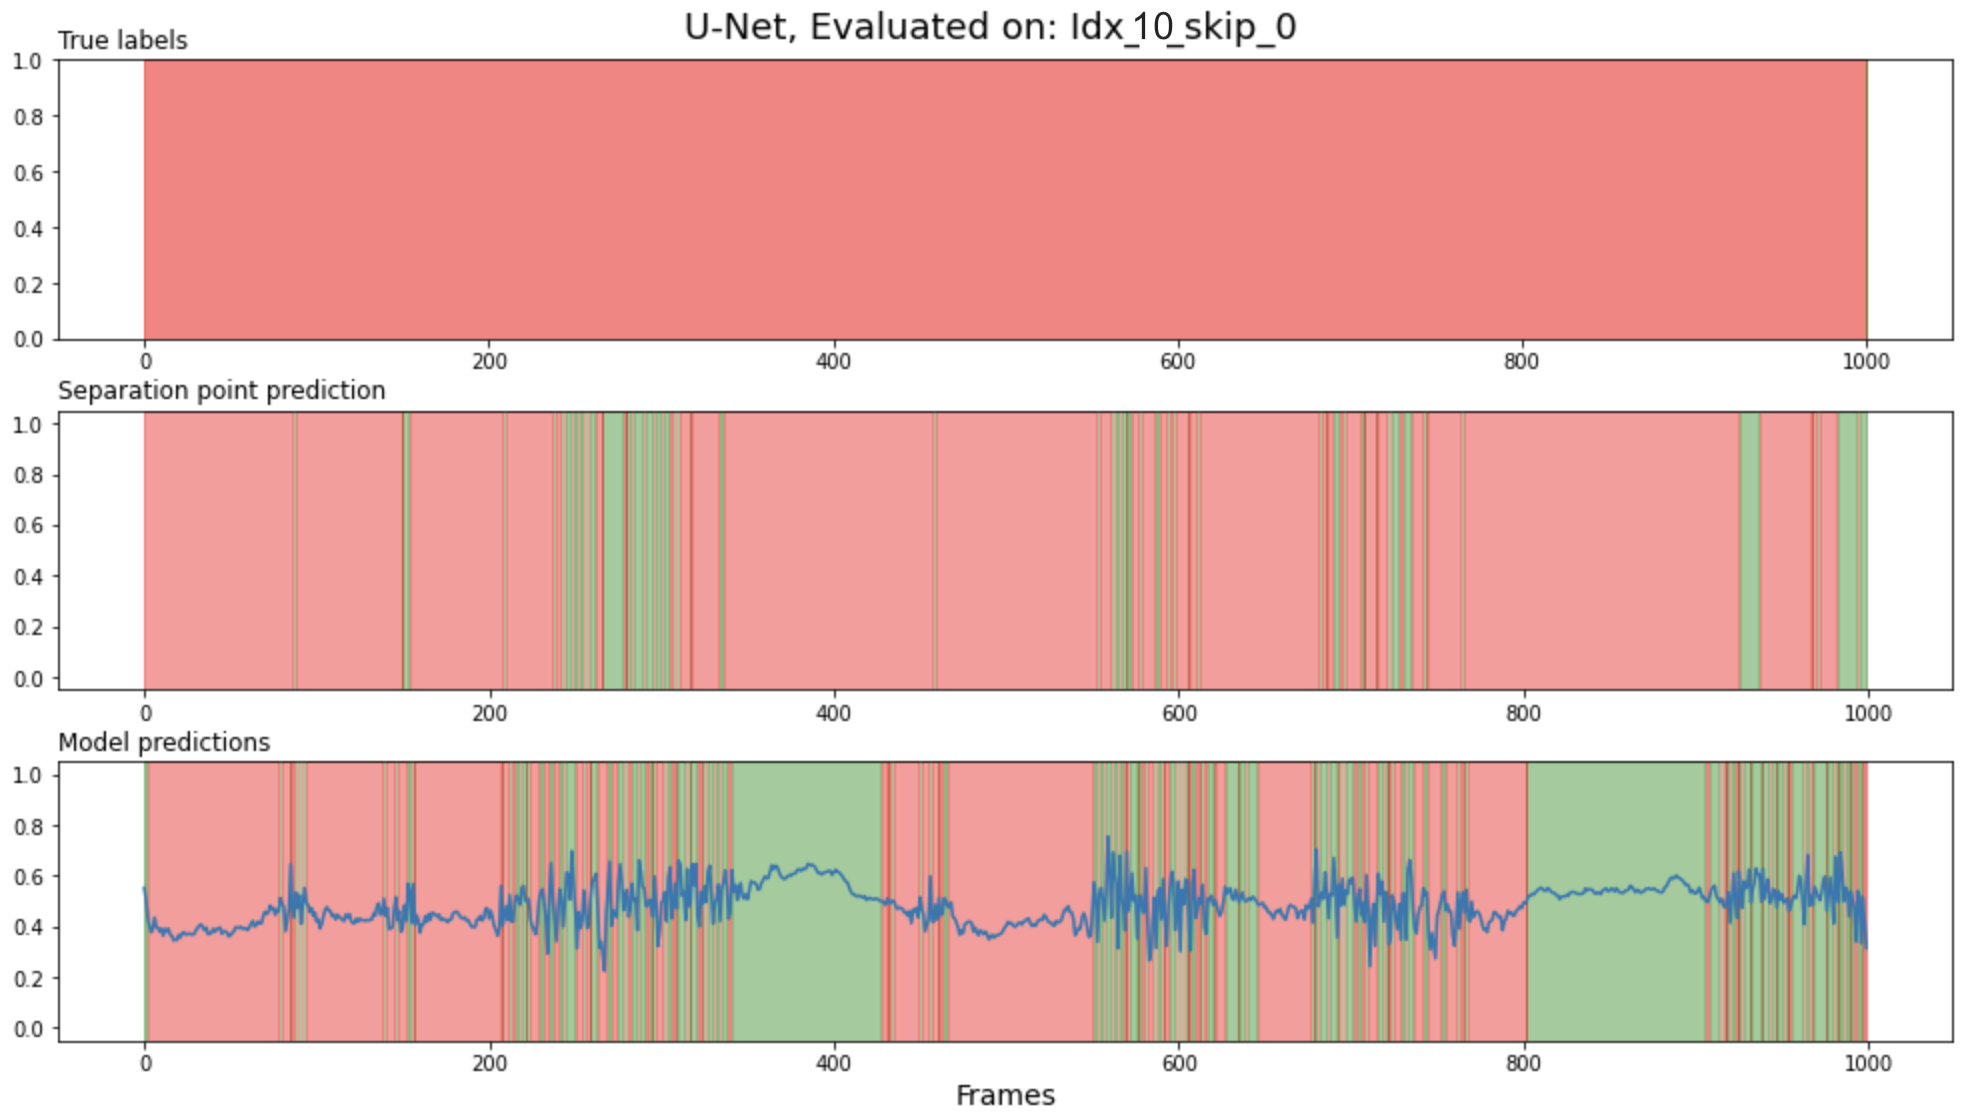
\includegraphics[width=\linewidth]{Materials/Results/UNet/unet3}
	\end{subfigure}
	\\
	\begin{subfigure}{\linewidth}
		\centering
		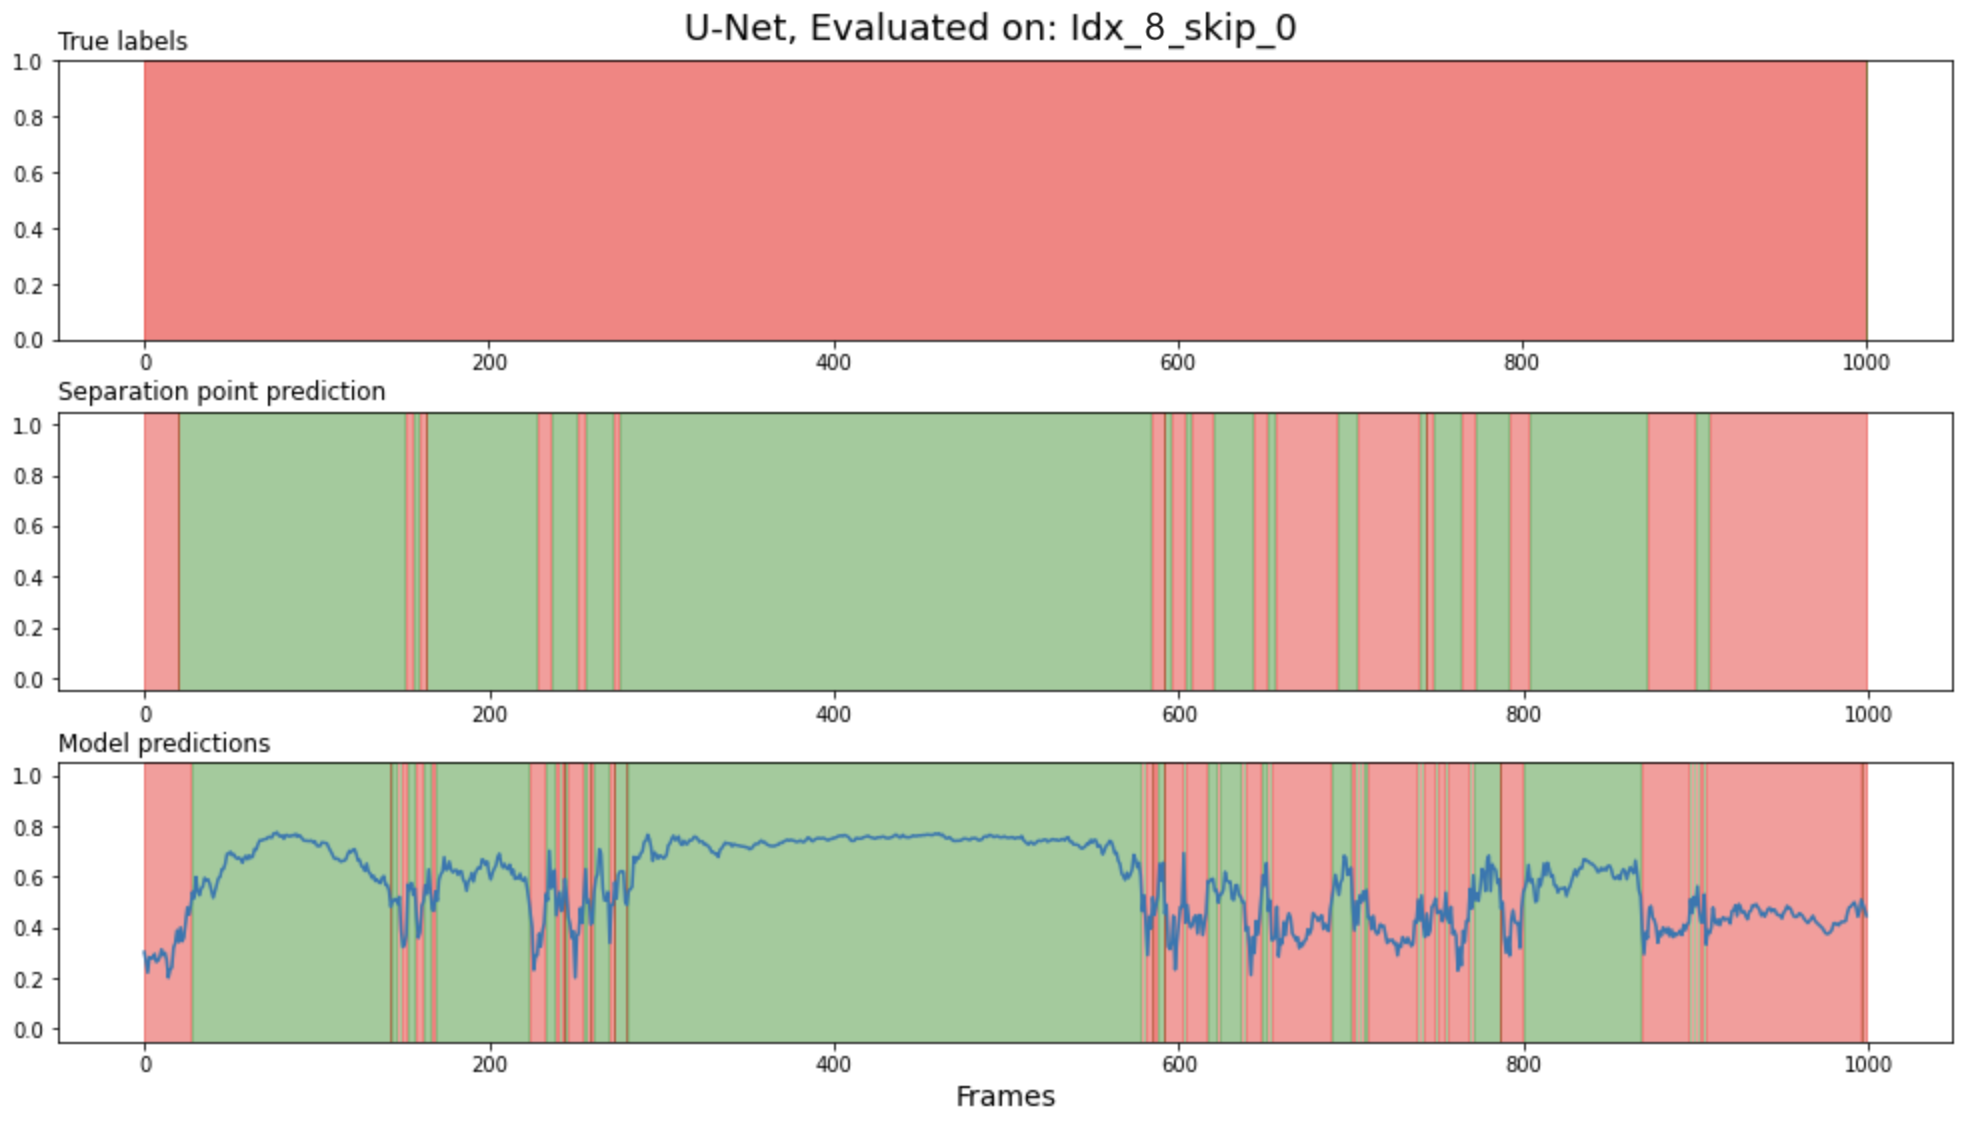
\includegraphics[width=\linewidth]{Materials/Results/UNet/unet4}
	\end{subfigure}
	\caption{Results of 1D U-Net model.}
	\label{unetres2}
\end{figure}

This tendency of making inflamed frames healthy seem to continue as we see in \autoref{unetres2}. For the first prediction we see the U-Net model likes to add healthy predictions even if they are wrong. In the second prediction we see the U-Net model is quite reluctant to add inflammation predictions when the ResNet model predicts too many healthy frames.

Even though we have only looked at four predictions this is the general tendency of the U-Net predictions. The model adds healthy predictions to the ResNet predictions, and it is very reluctant to add inflammation predictions, while being very steady and not overly confident in its predictions. As the ResNet was overly predicting inflammation, the U-Net seems to have caught on to a correct tendency of missing healthy frames. Although it has not quite managed to make its predictions two continuous blocks, its predictions are not heavily oscillating, and thus seem to have have caught on to the continuity a little.
\subsection{U-Net predictions for treatment prediction}
With the new segmentations produced by the U-Net model, treatment prediction was attempted again. This time the same 1D ResNet model was used, but training consisted of 70 epochs with a learning rate of $10^{-4}$ and with $0.01$ weight decay. Cross entropy was used as loss function and Adam was used for optimization.

\begin{table}[H]
	\hspace{-2.7cm}
	\begin{tabular}{|c|c|c|c|c|c|c|c|c|c|c|c|c|c|c|c|c|c|c|c|c|c|c|c|c|c|}
		\hline
		Idx&1
		&7
		&8
		&14
		&15
		&16
		&17
		&18
		&19
		&20
		&21
		&22
		&23
		&24
		&25
		&26
		&27
		&28
		&29
		&30
		&31
		&32
		&33
		&34
		&35\\\hline\hline
		Predictions&0
		&2
		&1
		&2
		&2
		&2
		&1
		&1
		&1
		&1
		&1
		&2
		&1
		&1
		&1
		&0
		&1
		&1
		&1
		&0
		&2
		&0
		&2
		&2
		&2\\\hline
		True&1
		&3
		&3
		&4
		&2
		&2
		&2
		&1
		&1
		&2
		&2
		&2
		&2
		&1
		&0
		&0
		&0
		&1
		&0
		&0
		&0
		&0
		&2
		&2
		&2\\\hline
	\end{tabular}
	\caption{Training a model only on the predicted U-Net segmentations, we find the following treatment predictions and true treatments shown for each video. The treatment classes are: 0 being 'healthy', 1 being 'local 5-ASA', 2 being 'Oral steroid', 3 being 'IV steroid' and 4 being 'oral 5-ASA'.}
	\label{unetPredsTreatmentTable}
\end{table}

\begin{figure}[H]
	\centering
	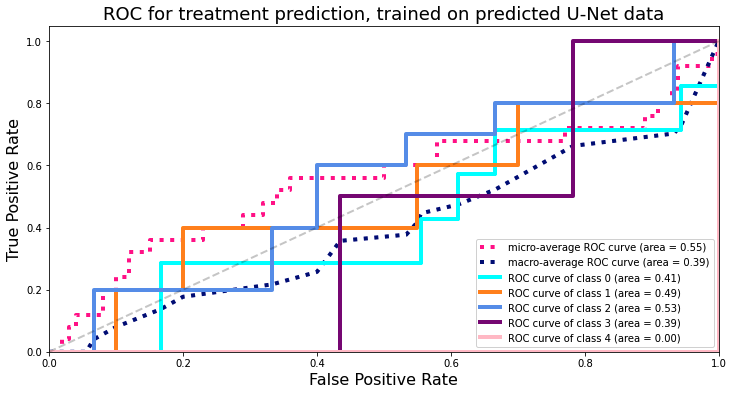
\includegraphics[width=0.85\linewidth]{Materials/Results/UNet/UNetROC1}
	\caption{ROC curves and area under the curve for the five binary 'one-vs-rest' classifiers along with micro- and macro-averages. Training was performed only on predicted segmentations.}
	\label{rocunetpreds}
\end{figure}
In \autoref{unetPredsTreatmentTable} we see the predicted treatments along the true prescribed treatment when we train only on the predicted segmentations from the U-Net model. In contrast to the previous results we now see predictions of classes $0, 1$ and $2$, where we previously did not see any predictions of treatment $1$. We also see an improvement in accuracy as we now have $52\%$.\\
Five binary 'one-vs-rest' classifiers were also trained for these predictions, and they were again trained using the same parameters as the multi class classifier. In \autoref{rocunetpreds} we see ROC curves for these binary classifiers, and we note the area under the curves being either $0.5$ or $0.4$ for all classes except class 4 which has $0.0$, which is significantly worse than for the previous treatment predictions.

When we include the true segmentations to the training data and repeat the experiment with the same parameters, we find the results seen in \autoref{unetPredsTrueTreatmentTable}. Here we again see the model predicting three classes, however, the accuracy drastically drops to $20\%$.

\begin{table}[H]
	\hspace{-2.7cm}
	\begin{tabular}{|c|c|c|c|c|c|c|c|c|c|c|c|c|c|c|c|c|c|c|c|c|c|c|c|c|c|}
		\hline
		Idx&1
		&7
		&8
		&14
		&15
		&16
		&17
		&18
		&19
		&20
		&21
		&22
		&23
		&24
		&25
		&26
		&27
		&28
		&29
		&30
		&31
		&32
		&33
		&34
		&35\\\hline\hline
		Predictions&2
		&2
		&2
		&2
		&1
		&1
		&1
		&2
		&2
		&2
		&1
		&1
		&2
		&2
		&1
		&2
		&2
		&2
		&2
		&2
		&1
		&0
		&2
		&1
		&2\\\hline
		True&1
		&3
		&3
		&4
		&2
		&2
		&2
		&1
		&1
		&2
		&2
		&2
		&2
		&1
		&0
		&0
		&0
		&1
		&0
		&0
		&0
		&0
		&2
		&2
		&2\\\hline
	\end{tabular}
	\caption{Training a model on the predicted U-Net segmentations and the true segmentations, we find the following treatment predictions and true treatments shown for each video. The treatment classes are: 0 being 'healthy', 1 being 'local 5-ASA', 2 being 'Oral steroid', 3 being 'IV steroid' and 4 being 'oral 5-ASA'.}
	\label{unetPredsTrueTreatmentTable}
\end{table}

In \autoref{rocunetpredstrue} we see the ROC curves when we add the true segmentations. Here, however, we see the area under the curve for class $0$ being a fair bit above $0.5$, indicating predictions for class $0$ are not random, while classes $1$ and $2$ are slightly above $0.5$. 

\begin{figure}[H]
	\centering
	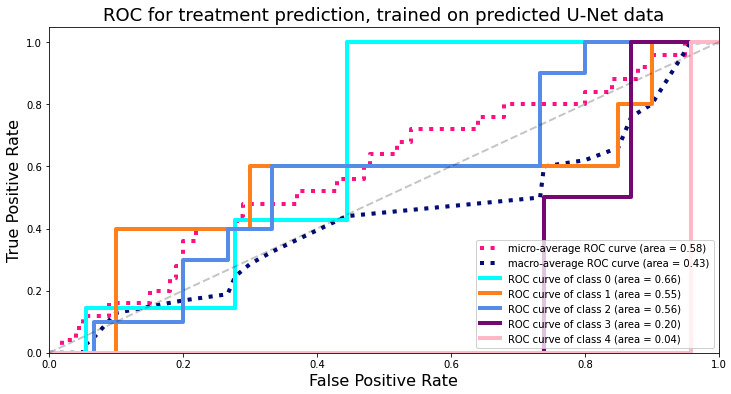
\includegraphics[width=0.85\linewidth]{Materials/Results/UNet/UNetROC2}
	\caption{ROC curves and area under the curve for the five binary 'one-vs-rest' classifiers along with micro- and macro-averages. Training was performed only on predicted segmentations.}
	\label{rocunetpredstrue}
\end{figure}
\section{Discussion of results}
\subsection{Model evaluation}
In \autoref{2dresnetevalres} we see the model evaluation of models trained on the different datasets. We see the training accuracies for all models being close to 100\% while the validation accuracies are lagging behind. The gap between training and validation accuracy, and the training accuracy being this high, would indicate that the model is overfitting the training data, which is likely also the reason a lot of models overly predicts either healthy or inflamed. It would thus have been sensible to add more regularization to the models for instance in the form of weight decay. This was also attempted, however, the combination of high dropout and weight decay seemed to halt learning to a degree where both training and validation accuracy would stay around 50\%. Because of this, it was decided not to add weight decay, and due to time constraints towards the end of the thesis, this issue was never re-visited. As these models are the very foundation of the project, more should probably have been done to tune them more accurately. This could have been done by training for more epochs and accordingly lower the learning rate. In state of the art applications, models are often trained for several days with low learning rate, however, such a setting would not have been feasible for this project as models was run in Google Colab with very limiting usage restrictions. Models could, however, have been trained for a lot longer than they were with a much smaller learning rate. Different model architectures could have been attempted. This could both be a different variant of ResNet, but also a completely different architecture. Also more combinations of dropout and weight decay could have been attempted to resolve the no learning issue. Likewise, different combinations of skipping frames in the videos used for training could have been explored more.\\
Splitting all the videos into seven folds, training on six and validating on one was also attempted. This was attempted because, usually the more diverse and the larger a volume of data used for training leads to the best results when training machine learning models. However, this was extensively tested by varying epochs, learning rate, number of skipped frames, weight decay and dropout. Because the validation results would not move above 56\% the experiment was prematurely ended, and thus not reported.

An interesting tendency we see in \autoref{2dresnetevalres} and when it was attempted to split all the videos into seven folds is that, the sheer number of frames does not seem to have any relation to the model accuracies. Although it is not directly the sheer number of training examples which is the reason machine learning models in general perform better on larger datasets, but the increased likelihood of having varied data, we would still have expected to see higher accuracies when training on more data and across several patients. To some extent we do see more data increases accuracy, as the two models trained on the same datasets but with varying amounts of data, both do increase in accuracy as their training set increases in size. However, we also see model \textit{idx\_2\_3\_4\_5\_6\_skip\_50} having higher accuracy than model \textit{idx\_4\_14\_18\_20\_32\_skip\_5} although the latter model's training set is eight times larger. This might simply boil down to the validation set being more similar to the data model \textit{idx\_2\_3\_4\_5\_6\_skip\_50} is trained on, but during the visual inspection on other videos from other patients, model \textit{idx\_2\_3\_4\_5\_6\_skip\_20} (trained on similar data) still performed better than model \textit{idx\_4\_14\_18\_20\_32\_skip\_5}. This also goes to show training on more patients do not necessarily increase model accuracy either.\\
It is hard to conclude why more data and training on more patients seemingly have no or limited effect on the model accuracy. One reason could be the features found vary too much or exists in both classes, contradicting themselves, and instead of making the model more robust, confuses it. Another reason could be the degree of inflammation varies too much, making it harder to find common features, and maybe it would have been beneficial to construct datasets with the type of treatment prescribed in mind. A last reason could be the amount of noisy images sampled from the videos vary, and the datasets trained across several patients might coincidentally have more noisy frames in them, although this has not been investigated.\\
Exactly why model \textit{idx\_2\_3\_4\_5\_6\_skip\_20} performs the best is also hard to conclude, but it is likely correlated to the above.

Looking into the visual results in \autoref{firstfive} and \autoref{lastthree} we see some quite volatile predictions from most models. This is likely due to the nature of the videos, where many frames all throughout the videos are all black or red, having glare effects or having a significant colour change when the camera comes too close to the colon to be able to focus. This is not an issue for a doctor to see past, however, when the model is trained on these noisy frames which belongs to both the healthy and inflamed classes, it is naturally a hard decision for the model to classify them correctly. The ResNet model also has no notion of what happens before or after the frame it processes, which gives the model no context to work out if an all red frame came before or after other inflamed frames. Another issue stems from the motion of the camera as some frames are blurred, which might make it hard to detect the features needed to determine if the frame contains signs of inflammation. In \autoref{exampleFrames} (a) and (d) we also saw an example of two very similar frames, being of opposite classes, and one could raise the question if (a) is inflamed or the lighting simply makes it look like it. This means although it might appear the models are indecisive or having issues predicting parts of the videos due to the volatile predictions, I argue it is to some extent impossible to avoid, and should be expected. Examples of noisy frames can be seen in \autoref{noisyFrames}.

\begin{figure}
	\centering
	\begin{subfigure}{0.4\linewidth}
		\centering
		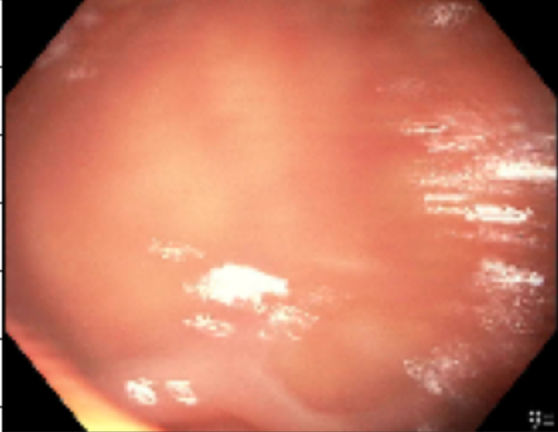
\includegraphics[width=\linewidth]{Materials/Discussion/idx_1_frame_550}
		\caption{Example of motion blur and glare (inflamed).}
	\end{subfigure}
	\hspace{0.5cm}
	\begin{subfigure}{0.4\linewidth}
		\centering
		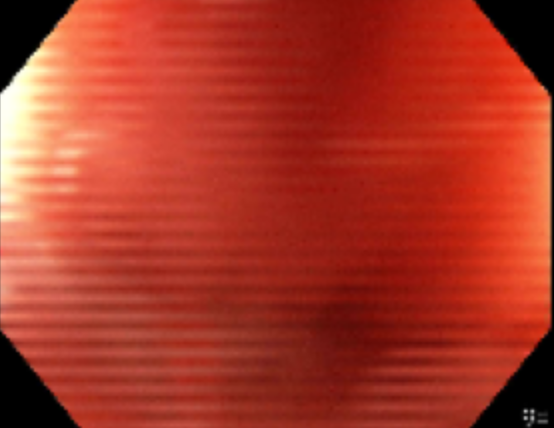
\includegraphics[width=\linewidth]{Materials/Discussion/idx_1_frame_1410}
		\caption{Example of all red frame (healthy).}
	\end{subfigure}
	\\
	\begin{subfigure}{0.4\linewidth}
		\centering
		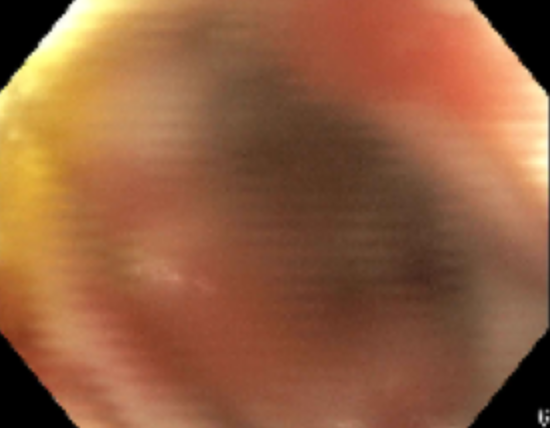
\includegraphics[width=\linewidth]{Materials/Discussion/idx_4_frame_750}
		\caption{Example of blurred frame (inflamed).\newline}
	\end{subfigure}
	\hspace{0.5cm}
	\begin{subfigure}{0.4\linewidth}
		\centering
		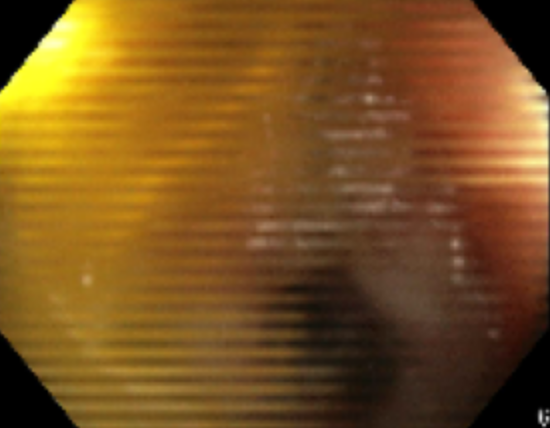
\includegraphics[width=\linewidth]{Materials/Discussion/idx_4_frame_840}
		\caption{Example of a large part of a frame changing colour to yellow (inflamed).}
	\end{subfigure}
	\caption{Examples of noisy frames in the endoscopy videos.}
	\label{noisyFrames}
\end{figure}

One could remove all of these frames from the training data, making it a lot easier for the model to find the needed features in the images to detect inflammation, however, when it is then presented with a video 'from the real world', it would likely not be able to generalize due to unseen noise.

To evaluate the performance of model \textit{Idx\_2\_3\_4\_5\_6\_skip\_20}, we take a look at its $65\%$ validation accuracy and at its predictions in \autoref{idx23}, \autoref{idx24} and \autoref{idx28}. Its accuracy is by itself not impressive, and especially not when taking into consideration about $72\%$ of the validation video are inflamed frames. Looking at its predictions, the model overly predicts inflammation, which leads to a conservative model which has a hard time predicting correctly on videos which are balanced or biased towards healthy frames. On the other hand, the model seems to perform decent on videos biased towards inflamed frames, where it most often finds some correct healthy frames. Although we should not expect perfect segmentation due to the noisy nature of the videos, we conclude none of the models are performing optimally, and model \textit{Idx\_2\_3\_4\_5\_6\_skip\_20} to a small degree produces usable results, however, they are not of a quality where they can contribute with any meaningful information to a doctor.

\subsection{Separation point predictions}
A general tendency for the Random Walker post-processing was to predict the separation point at the location of the last uncertainty in predictions. That is, the rightmost part of the segmentation where there would be either volatile predictions or elevated probability of predicting healthy. Because the Random Walker has a hard time crossing points or frames where the model predictions are dissimilar, this is somewhat expected, but due to the random noise in the videos previously discussed, this makes this approach conservative and not very robust. This was also verified as on average, the Random Walker approach would predict a separation point $51.85\%$ of the total number of frames in a video away from the true separation point. For the results produced by model \textit{Idx\_2\_3\_4\_5\_6\_skip\_20} this approach is thus not usable to predict the separation points.\\
Had we had more accurate predictions, the results would likely have been better, however, due to the noisy nature of the videos, and how the Random Walker would likely get 'stuck' on the noise, it is still questionable if this approach can produce meaningful results.

The scoring heuristic works by finding dissimilarities between the prediction probabilities of two consecutive frames. If the there is a high probability both frames belong to the same class, the score is high, whereas, if there is a high probability they belong to different classes, the score is low. Thus, this approach should be good at finding the transitions between frames where the model is insecure or predicts on noisy data. This is also generally what we see, and often one of the candidate points are near the true separation point, however, it is rare this candidate point holds the actual lowest score. As it on average would predict a separation point $51.87\%$ of the total number of frames in a video away from the true separation point, its 'believed separation point' is not usable to predict the separation points.\\
Providing candidate points could be useful for a doctor to do a quick evaluation based on the predicted segmentation and the candidate points. This could save the doctor time by not having to look the whole video through. But, as it is hard, if not impossible, to tell if any of the candidate points actually resembles the true separation point, only having the predicted segmentation available, the fact one of the candidate points often (but not always) is accurate is not of much help in practice.

\subsection{Treatment predictions}
While most treatment annotations are clear, some videos have been annotated with treatment 'x or y'. These cases are indices $7$ and $8$ which have been annotated as class $2$ or $3$, index 14 annotated class $2$ or $4$, index 28 annotated class $0$ or $1$ and indices 34 and 35 annotated class $1$ or $2$. In all these cases, the largest class number has been chosen as the true class, however, this might add or subtract a few percentages of accuracy depending on how the true classes are chosen.

In \autoref{treatmentTable} we saw the 1D ResNet model could achieve an accuracy of $40\%$, which is good considering random predictions would have yielded $20\%$ accuracy. However, if these predictions were to be used by a doctor, as for instance a second opinion, $40\%$ is rather low and would be too unreliable. We also see the model only predicting classes $0$ and $2$, which would indicate the model does not generalize too well.\\
Looking at \autoref{rocpreds} we see class $0$ and class $1$ having an area under the curve above $0.5$ which indicates the models have some measure of class separability whereas for classes $2$ and $3$ we see the scores being very close to $0.5$. Looking at class $4$, we have a score of $0.33$ which would indicate it is quite hard to predict correctly. When we look at class $3$ and $4$, we need to remember only 2 and 1 examples exists in the data, and thus the model will naturally have a hard time predicting these classes. If we look at the micro average, we see a score of $0.68$, which would indicate we can expect a model to have some measure of class separability when trained on this data, which we already have seen was the case. However, looking at the macro average which takes the class imbalance into consideration, we should not expect any meaningful results. This might, however, be skewed as class $3$ and $4$ have this few examples.

In \autoref{treatmentTableWithTrue} we added the true segmentations during training, and the accuracy increased to $48\%$. However, the model still only predicts class $0$ and $2$, indicating it overfits the training data. Looking at \autoref{rocpredsandtrue} we see the scores for class $0$ and $1$ almost swap, and the rest of the classes and the macro average staying very similar to what we had without adding the true segmentations. The micro average falls slightly, but still is at a level where some notion of class separability would be expected. The micro average falling, and yet the multi class classifier achieving a higher accuracy could be caused by the model predictions being closer to each other, i.e. the model is not as confident in its choice of class, but still ends up choosing the correct class.

Overall it would seem more tuning could have been done to achieve better results. Although nearing $50\%$ accuracy on a $5$ class classification problem seems decent, the ROC curves are not very confident, and even the highest scores being rather mediocre. Again training for more epochs with an accordingly lower learning rate could be a possible improvement. The indications of overfitting in both results would also point towards more regularization would be needed. Adding dropout to force the models to learn a wider array of features in the data could be one choice. As we are seeing the model is capable of solving the problem to some extent, a change of model architecture is most likely not needed to raise the performance.

\subsection{U-Net for video segmentation}
Opposite to ResNet, that would make its predictions on each individual image without considering the images before and after it, the U-Net models were trained on the segmentations, and because U-Net works on several levels of abstractions it would be expected to capture the 'structure' of the segmentations, i.e. how the true segmentations are blocks of first inflamed frames and then healthy frames. This structure is to a large degree missing from the initial 2D ResNet predictions, and thus the hope with the results of using the U-Net, was to bring this structure into the predictions.\\
Looking at \autoref{unetres1} and \autoref{unetres2} we see the U-Net overly predict healthy frames, which probably is a reaction to the ResNet overly predicting inflammation. The structure we were seeking, is also only brought back to a limited extent. Because the U-Net predictions overrule the correctly predicted frames from the ResNet, it seems the problem with the original predictions have just shifted from being overly many inflamed predictions to overly many healthy predictions. 

\subsection{U-Net predictions for treatment prediction}
Although the predictions of the U-Net models did not seem to make the results much more usable than the original 2D ResNet results, we see a big difference in how the treatments are predicted. In \autoref{unetPredsTreatmentTable} we now see predictions of class 0, 1 and 2. Because of the low number of examples of class 3 and 4 treatments, it is not surprising we do not see these classes predicted. We now have an accuracy of $52\%$ which, taking into consideration we have 5 classes, is decent. However, it is still not high enough to, for instance, act as a second opinion for a doctor. Looking at \autoref{rocunetpreds} we now see a drastic drop in the area under the ROC curves. We now only have class 4 not being near a score of $0.5$. Given how the 'one-vs-rest' classifiers struggle, the high accuracy could be caused by the multi class classifier not being very confident and having almost equal probabilities for each class, but the correct class coming out on top for the most part.

In \autoref{unetPredsTrueTreatmentTable} the true segmentations were added to the training. We still see the model predicting class 0, 1 and 2, however, we now see the accuracy drop to $20\%$, indicating random guesses were made. Looking at \autoref{rocunetpredstrue} we however see class 0 having a score of $0.66$, suggesting these predictions were not entirely random. The rest of the classes do struggle however. It is likely adding the true segmentations simply confused the model during training, as the features found in the predicted segmentations did not match the features found for the true segmentations. Also, the drop in accuracy could stem from the multi class classifier not being confident in its predictions, giving almost equal probabilities to each class, but this time the correct classes would not come out on top.


















\section{Conclusion}
In conclusion we have seen where segmentation can be used in medical image analysis, we have seen the risks of dilation and erosion and explained the benefits of them, we have concluded Graph cut segmentations are preferred, but also have limited applications and Random walker alleviates these constrains by being non-deterministic, and finally we have looked into how PCA can be used for segmentation.
\begin{thebibliography}{9}
	\bibitem{wikimicroscopy}
	Wikipedia, 'Two-photon excitation microscopy', \url{https://en.wikipedia.org/wiki/Two-photon_excitation_microscopy}, Visited: June 11, 2021.
	
	\bibitem{trasnferlearning}
	Wikipedia, 'ImageNet', \url{https://en.wikipedia.org/wiki/ImageNet}, Visited: June 26, 2021.
	
	\bibitem{imaging}
	Mathiesen Janiurek et al, 'Apolipoprotein M-bound sphingosine-1-phosphate regulates blood–brain barrier paracellular permeability and transcytosis', eLife 2019, Published: 25 November 2019.

	\bibitem{swhati}
	Swathi Ayloo and Chenghua Gu, 'Transcytosis at the blood–brain barrier', Current Opinion in Neurobiology, Published: 2019.

	\bibitem{zhao}
	Zhen Zhao et al, 'Establishment and Dysfunction of the Blood-Brain Barrier', Cell 163, Published: November 19, 2015.
	
	\bibitem{confocal}
	Wikipedia, 'Confocal microscopy', \url{https://en.wikipedia.org/wiki/Confocal_microscopy}, Visited: June 22, 2021.
	
	\bibitem{unetarticle}
	Olaf Ronneberger et al, 'U-Net: Convolutional Networks for Biomedical Image Segmentation', Computer Science Department and BIOSS Centre for Biological Signalling Studies,
	University of Freiburg, Germany, Published: 2015.
	
	\bibitem{resnet}
	Kaiming He et al, 'Deep Residual Learning for Image Recognition', Microsoft Research, Published: December 10, 2015.
	
	\bibitem{linknet}
	A. Chaurasia and E. Culurciello, 'LinkNet: Exploiting Encoder Representations for Efficient Semantic Segmentation', Purdue University, Published: June 14, 2015
	
	\bibitem{augmentation}
	C. Shorten and T. Khoshgoftaar, 'A survey on Image Data Augmentation for Deep Learning', Journal of Big Data, Published: 2019.
	
	\bibitem{convolutionarticle}
	Vincent Dumoulin and Francesco Visin, 'A guide to convolution arithmetic for deep learning', MILA, Université de Montréal and AIRLab, Politecnico di Milano, March 24, 2016.
	
	\bibitem{adam}
	D.Kingma, J. Ba, 'ADAM: A METHOD FOR STOCHASTIC OPTIMIZATION', Published as a conference paper at ICLR, 2015
\end{thebibliography}
\section{Appendix}
\subsection{Full sized images vs. halved sized images}
In another experiment it was investigated whether the model performances would change if the full sized images were used rather than the half sized images. In \autoref{fullsize} four modified U-Net models initialized with the ImageNet weights were trained first on a dataset where the images were halved and then where the images kept their full size. On both datasets using the full sized images seems to make the models converge considerably faster. For the models trained on the original dataset the validation loss seems to be lower when the images are halved while the training loss seems to be about the same. However, when using data from the original, large rotation, horizontal and vertical datasets the validation loss seem to be higher for the halved images, but the training loss seems be lower.
\begin{figure}[H]
	\centering
	\begin{subfigure}[b]{0.24\linewidth}
		\centering
		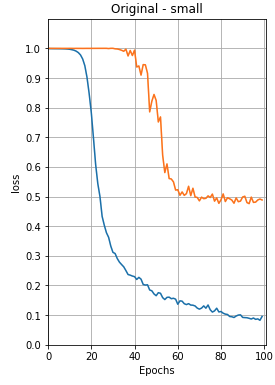
\includegraphics[width=\linewidth]{Materials/Results/Augmentation/Original}
		\caption{Model trained on original dataset with halved sizes.\newline\newline}
	\end{subfigure}
	\hfill
	\begin{subfigure}[b]{0.24\linewidth}
		\centering
		\includegraphics[width=\linewidth]{Materials/Results/Fullsize/originalfull}
		\caption{Model trained on original dataset with full sizes.\newline\newline}
	\end{subfigure}
	\hfill
	\begin{subfigure}[b]{0.24\linewidth}
		\centering
		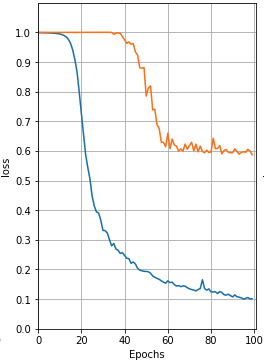
\includegraphics[width=\linewidth]{Materials/Results/Fullsize/augsmall}
		\caption{Model trained on original, large rotations, horizontal and vertical dataset with halved sizes.}
	\end{subfigure}
	\hfill
	\begin{subfigure}[b]{0.24\linewidth}
		\centering
		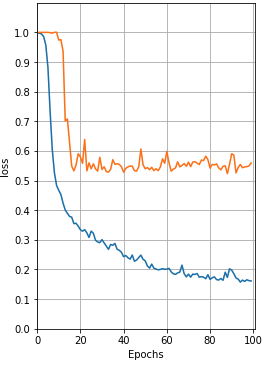
\includegraphics[width=\linewidth]{Materials/Results/Fullsize/augfull}
		\caption{Model trained on original, large rotations, horizontal and vertical dataset with full sizes.}
	\end{subfigure}
	\caption{Experiment showing the effect of training on full sized images vs. halved sized images.}
	\label{fullsize}
\end{figure}

\subsection{Test results}
\begin{figure}[H]
	\centering
	\begin{subfigure}[b]{\linewidth}
		\centering
		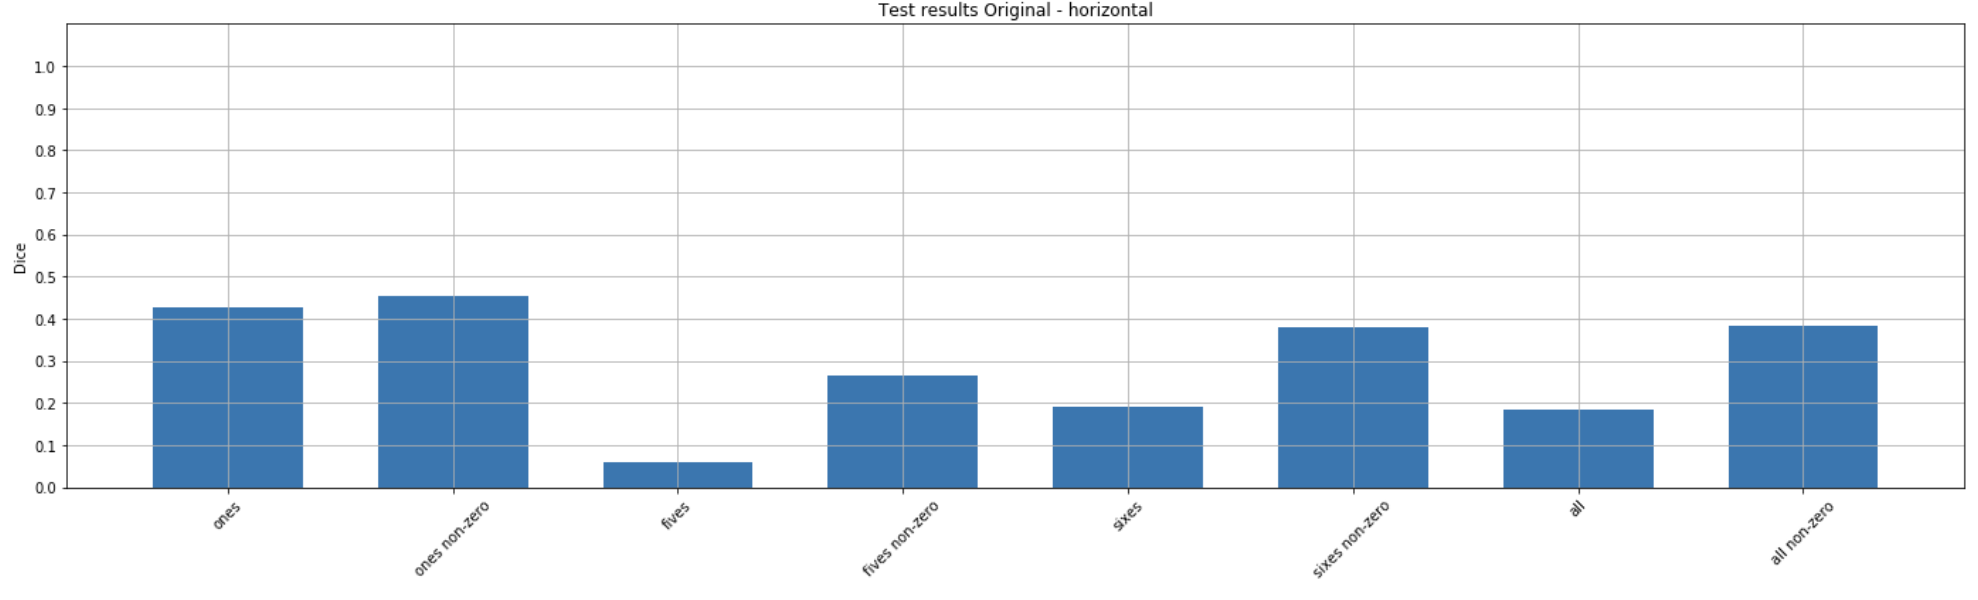
\includegraphics[width=\linewidth]{Materials/Appendix/OH}
		\caption{Results for the model trained on the original and horizontal data sets.}
	\end{subfigure}
	\caption{Average DICE on test set split into three separate volumes consisting of the single series images, five series images and six series images.}
\end{figure}
\begin{figure}[H]
	\centering
	\begin{subfigure}[b]{\linewidth}
		\centering
		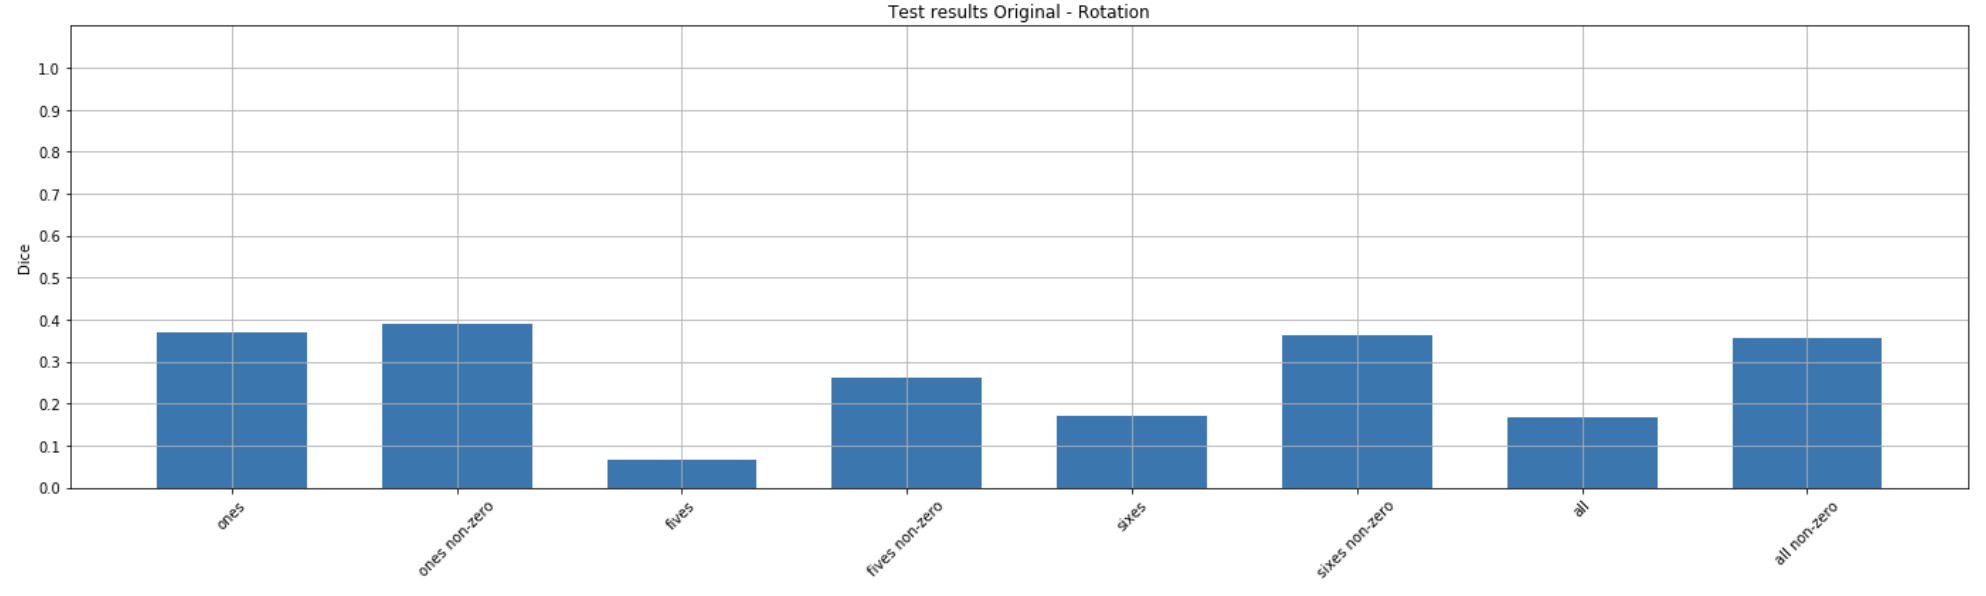
\includegraphics[width=\linewidth]{Materials/Appendix/OR}
		\caption{Results for the model trained on the original and large rotations data sets.}
	\end{subfigure}
	\\
	\begin{subfigure}[b]{\linewidth}
		\centering
		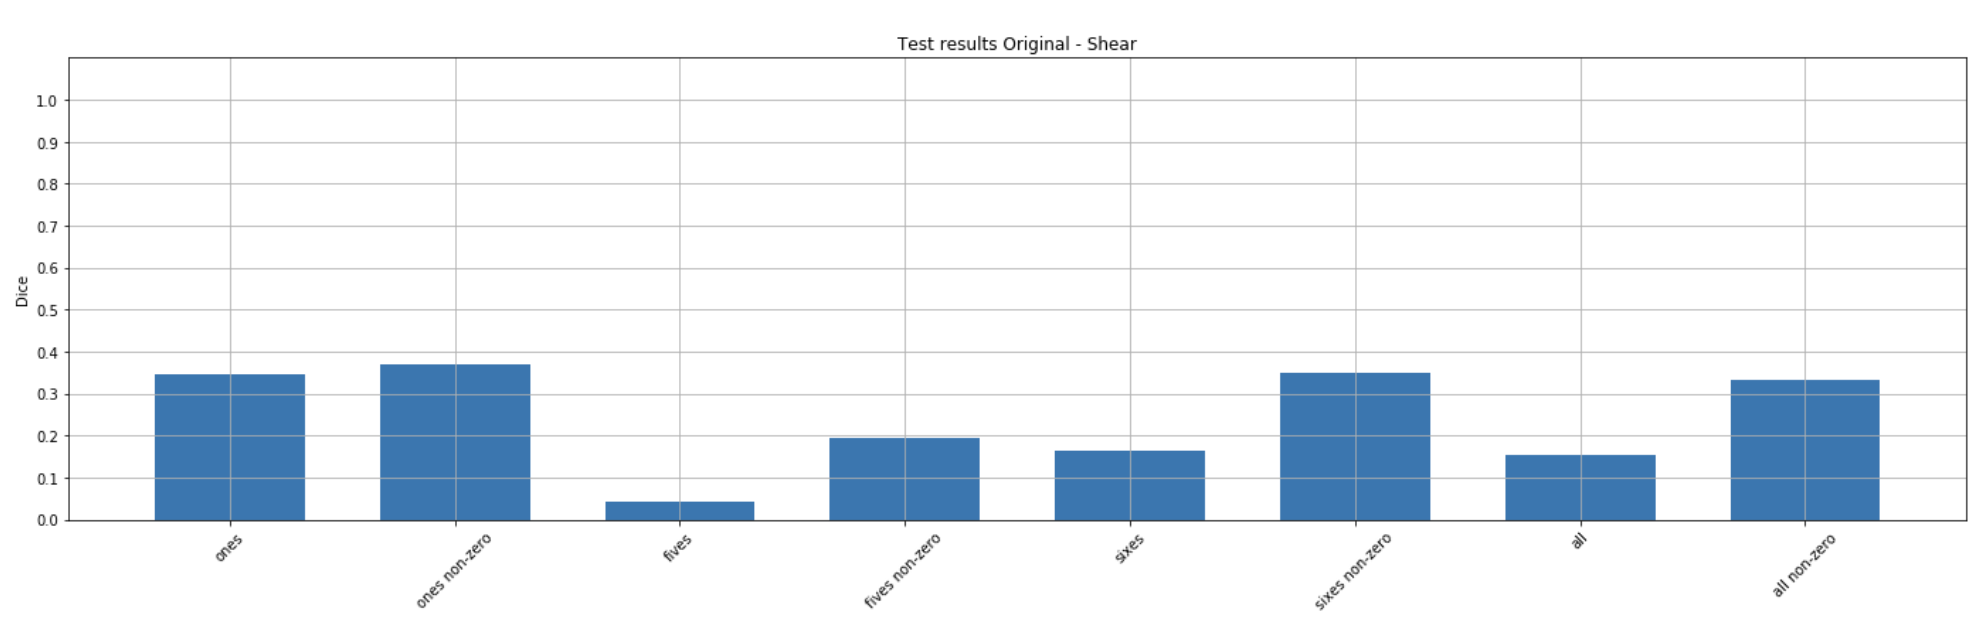
\includegraphics[width=\linewidth]{Materials/Appendix/OS}
		\caption{Results for the model trained on the original and large shearing data sets.}
	\end{subfigure}
	\\
	\begin{subfigure}[b]{\linewidth}
		\centering
		\includegraphics[width=\linewidth]{Materials/Appendix/ORS}
		\caption{Results for the model trained on the original, large rotations and large shearing data sets.}
	\end{subfigure}
	\\
	\begin{subfigure}[b]{\linewidth}
		\centering
		\includegraphics[width=\linewidth]{Materials/Appendix/ORHV}
		\caption{Results for the model trained on the original, large rotations, horizontal and vertical data sets.}
	\end{subfigure}
	\caption{Average DICE on test set split into three separate volumes consisting of the single series images, five series images and six series images.}
\end{figure}
\begin{figure}[H]
	\centering
	\begin{subfigure}[b]{\linewidth}
		\centering
		\includegraphics[width=\linewidth]{Materials/Appendix/ORHVS}
		\caption{Results for the model trained on the original, large rotations, horizontal, vertical and large shearing data sets.}
	\end{subfigure}
	\caption{Average DICE on test set split into three separate volumes consisting of the single series images, five series images and six series images.}
\end{figure}

\subsection{Prediction examples}
Here we see predicted masks versus the corresponding true mask for different models and images in the training set.

\begin{figure}[H]
	\centering
	\begin{subfigure}[b]{0.23\linewidth}
		\centering
		\includegraphics[width=\linewidth]{Materials/Appendix/results/O30R30SPred}
		\caption{Predicted mask from model trained on original, small rotations and small shearing. 0.93 DICE.}
	\end{subfigure}
	\hfill
	\begin{subfigure}[b]{0.23\linewidth}
		\centering
		\includegraphics[width=\linewidth]{Materials/Appendix/results/imgaugPred}
		\caption{Predicted mask from imgaug model. 0.87 DICE.\newline\newline}
	\end{subfigure}
	\hfill
	\begin{subfigure}[b]{0.23\linewidth}
		\centering
		\includegraphics[width=\linewidth]{Materials/Appendix/results/originalPred}
		\caption{Predicted mask from model trained on original training set. 0.93 DICE.\newline}
	\end{subfigure}
	\hfill
	\begin{subfigure}[b]{0.23\linewidth}
		\centering
		\includegraphics[width=\linewidth]{Materials/Appendix/results/OHPred}
		\caption{Predicted mask from model trained on original and horizontal data sets. 0.90 DICE.}
	\end{subfigure}
	\\
	\begin{subfigure}[b]{0.23\linewidth}
		\centering
		\includegraphics[width=\linewidth]{Materials/Appendix/results/O30R30SMask}
		\caption{True mask from model trained on original, small rotations and small shearing.}
	\end{subfigure}
	\hfill
	\begin{subfigure}[b]{0.23\linewidth}
		\centering
		\includegraphics[width=\linewidth]{Materials/Appendix/results/imgaugMask}
		\caption{True mask from imgaug model.\newline\newline}
	\end{subfigure}	
	\hfill
	\begin{subfigure}[b]{0.23\linewidth}
		\centering
		\includegraphics[width=\linewidth]{Materials/Appendix/results/originalMask}
		\caption{True mask from model trained on original training set.\newline}
	\end{subfigure}
	\hfill
	\begin{subfigure}[b]{0.23\linewidth}
		\centering
		\includegraphics[width=\linewidth]{Materials/Appendix/results/OHPred}
		\caption{True mask from model trained on original and horizontal data sets.\newline}
	\end{subfigure}
\end{figure}
\end{document}